\documentclass[a4paper, 12pt]{report}

\usepackage[dvipsnames]{xcolor}

%%%%%%%%%%%%%%%%%
% Set Variables %
%%%%%%%%%%%%%%%%%

\def\useItalian{0}  % 1 = Italian, 0 = English

\def\courseName{Network Algorithms}

\def\coursePrerequisites{
    \begin{itemize}
        \item Progettazione di Algoritmi
    \end{itemize}
}

\def\book{TODO}

% \def\authorName{Simone Bianco}
% \def\email{bianco.simone@outlook.it}
% \def\github{https://github.com/Exyss/university-notes}
% \def\linkedin{https://www.linkedin.com/in/simone-bianco}

\def\authorName{Alessio Bandiera}
\def\email{alessio.bandiera02@gmail.com}
\def\github{https://github.com/aflaag-notes}
\def\linkedin{https://www.linkedin.com/in/alessio-bandiera-a53767223}

% Do not change

%%%%%%%%%%%%
% Packages %
%%%%%%%%%%%%

\usepackage{../../packages/Nyx/nyx-packages}
\usepackage{../../packages/Nyx/nyx-styles}
\usepackage{../../packages/Nyx/nyx-frames}
\usepackage{../../packages/Nyx/nyx-macros}
\usepackage{../../packages/Nyx/nyx-title}
\usepackage{../../packages/Nyx/nyx-intro}

%%%%%%%%%%%%%%
% Title-page %
%%%%%%%%%%%%%%

\logo{../../packages/Nyx/logo.png}

\ifx\useItalian0
    \institute{\curlyquotes{\hspace{0.25mm}Sapienza} Università di Roma}
    \faculty{Ingegneria dell'Informazione,\\Informatica e Statistica}
    \department{Dipartimento di Informatica}
    \subtitle{Appunti integrati con il libro \book}
    \author{\textit{Autore}\\\authorName}
\else
    \institute{\curlyquotes{\hspace{0.25mm}Sapienza} University of Rome}
    \faculty{Faculty of Information Engineering,\\Informatics and Statistics}
    \department{Department of Computer Science}
    \subtitle{Lecture notes integrated with the book \book}
    \author{\textit{Author}\\\authorName}
\fi

\title{\courseName}
\date{\today}

% \supervisor{Linus \textsc{Torvalds}}
% \context{Well, I was bored\ldots}

\addbibresource{./references.bib}

%%%%%%%%%%%%
% Document %
%%%%%%%%%%%%

\begin{document}
    \maketitle

    % The following style changes are valid only inside this scope 
    {
        \hypersetup{allcolors=black}
        \fancypagestyle{plain}{%
        \fancyhead{}        % clear all header fields
        \fancyfoot{}        % clear all header fields
        \fancyfoot[C]{\thepage}
        \renewcommand{\headrulewidth}{0pt}
        \renewcommand{\footrulewidth}{0pt}}

        \romantableofcontents
    }

    \introduction

    %%%%%%%%%%%%%%%%%%%%%

    \chapter{The routing problem}

    \section{Introduction on graphs}

    In many network applications, graphs are used as a natural model. In other applications, the graph model may be less obvious, but appears to be still very useful. Graph algorithms are useful instruments to solve important and living problems. We will see a number of advanced techniques for efficient algorithm design to solve problems from networks and graphs. 

    \begin{frameddefn}{Graph}
        A \tbf{graph} is a mathematical structure $G = (V,E)$ made of a set $V$ called the \textit{vertex set} (or \textit{node set}), and a set $E \subseteq V \times V$ called \textit{edge set}.
    \end{frameddefn}

    Graphs are usually represented through circles and lines, were each line between two vertices $u,v$ represents the edge $(u,v)$. We will assume to be working with \textit{simple graphs}, a type of graph that doesn't allow loop edges, i.e. edges from a node to itself, or a multiple number of edges between two vertices.  
   

    The edges of a graph can also be \textit{directed} or \textit{undirected}. In the former, the two edges $(u,v)$ and $(v,u)$ are considered two distinct edges while in the latter they are considered as the same edge. A directed graph is usually also referred to as \tbf{digraph}. 
    
    \begin{figure}[H]
        \centering

        \begin{tabular}{ccc}
            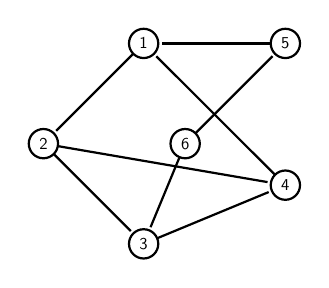
\begin{tikzpicture}[-,>=stealth,shorten >=1pt,auto,node distance=3cm,thick,main node/.style={scale=0.6,circle,draw,font=\sffamily\normalsize}]
                \node[main node] (1) {1};
                \node[main node] (2) [below left of=1] {2};
                \node[main node] (3) [below right of=2] {3};
                \node[main node] (6) [right of=2] {6};
                \node[main node] (5) [above right of=6] {5};
                \node[main node] (4) [below of=5] {4};
    
                \path[every node/.style={font=\sffamily\small}]
                    (1) edge (2)
                    (2) edge (3)
                    (2) edge (4)
                    (3) edge (4)
                    (4) edge (1)
                    (5) edge (1)
                    (6) edge (3)
                    (6) edge (5)
                    ;
            \end{tikzpicture}

            &\qquad\qquad&

            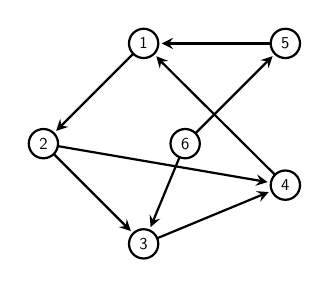
\begin{tikzpicture}[->,>=stealth,shorten >=1pt,auto,node distance=3cm,thick,main node/.style={scale=0.6,circle,draw,font=\sffamily\normalsize}]
                \node[main node] (1) {1};
                \node[main node] (2) [below left of=1] {2};
                \node[main node] (3) [below right of=2] {3};
                \node[main node] (6) [right of=2] {6};
                \node[main node] (5) [above right of=6] {5};
                \node[main node] (4) [below of=5] {4};
    
                \path[every node/.style={font=\sffamily\small}]
                    (1) edge (2)
                    (2) edge (3)
                    (2) edge (4)
                    (3) edge (4)
                    (4) edge (1)
                    (5) edge (1)
                    (6) edge (3)
                    (6) edge (5)
                    ;
            \end{tikzpicture}
        \end{tabular}

        \caption{On the left: a simple graph. On the right: a simple digraph.}
    \end{figure}

    Graphs were born in 1736, when Euler used them to formalize and solve the famous \textit{Seven Bridges of Königsberg} problem: is there a way to walk through all the bridges of the town and end up on the starting point? 

    \begin{figure}[H]
        \centering

        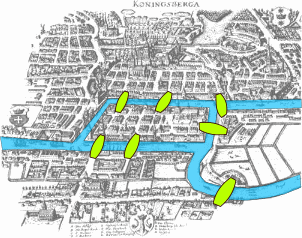
\includegraphics[scale=0.6]{../assets/Konigsberg_bridges.png}
        \caption{The city of Königsberg and its seven bridges.}
    \end{figure}

    To solve the problem, Euler represented the problem as the following \textit{multi-graph}, i.e. a non-simple graph that allows multiple edges between two vertices. Euler proved that the answer to the question is negative: a walk that passes through all the edges of such graph while also returning to the starting node \tbf{cannot exist}.

    \begin{figure}[H]
        \centering
        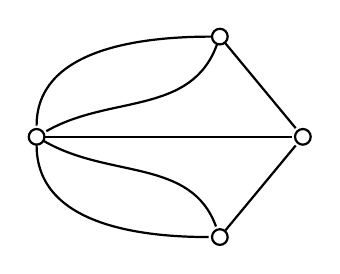
\begin{tikzpicture}[-,>=stealth,shorten >=1pt,auto,node distance=3cm,thick,main node/.style={scale=0.6,circle,draw,font=\sffamily\normalsize}]
            \node[main node] (1) {};
            \node[main node] (2) [below left of=1, xshift = -50] {};
            \node[main node] (3) [below right of=2, xshift = 50] {};
            \node[main node] (4) [right of=2, xshift = 75] {};

            \path[every node/.style={font=\sffamily\small}]
                (1) edge [out=180, in=90] (2)
                (1) edge [out=-110, in=30] (2)
                (2) edge [out=270, in=180] (3)
                (2) edge [out=-30, in=110] (3)
                (2) edge (4)
                (1) edge (4)
                (3) edge (4)
                ;
        \end{tikzpicture}

        \caption{The multi-graph representing the \tit{Seven Bridges of Königsberg} problem.}
    \end{figure}

    In general, a \tbf{walk} on a graph $G$ is given by a sequence of nodes $v_1, \ldots, v_k$ such that $(v_i, v_{i+1}) \in E(G)$. A \tbf{path} is walk whose vertices are all distinct. As we'll see in the following sections, walks and paths are the basis of graph theory.

    \newpage

    \section{The least cost path problem}

    When packets are sent from a computer to another through a network, each computer has to route data on a path passing through intermediate computers. This problem is usually referred to as the \tbf{routing problem}.
    
    By modelling the network as a graph whose vertices correspond to the computers and its edges correspond to the links between them, such problem is reduced to the concept of a path from an initial node to an arrival node.

    Based on the required conditions, the routing reduces to a specific type of path problem:
    \begin{enumerate}
        \item In \tbf{non-adaptive routing}, the routing algorithm must minimize the number of intermediate computers on the route. This problem reduces to the \textit{shortest path problem}, i.e. finding the path that passes through the lowest amount of edges from node $s$ to node $t$. This type of routing gives good results with consistent topology and traffic conditions, but performs poorly in case of congestion.  Usually this type of routing is implemented through one global \tit{routing table}.
        \item In \tbf{adaptive routing}, the routing algorithm must take into account the traffic conditions: if a route is congested, we want to avoid passing through it. This problem reduces to the \textit{least cost path problem}, i.e. finding the path with the least cost from node $d$ to node $t$. This type of routing gives good results with high network workload, but routes must be computed frequently in order to perform well. In this type of routing, each router creates its own \tit{routing table}.
        \item In \tbf{half-adaptive routing}, depending on traffic and workload on the network, the routing type can switch between \tit{adaptive} and \tit{non-adaptive}.
        \item In \tbf{fault-sensitive routing}, the routing algorithm must consider the possibility of a link failing: we want the route with the highest probability of working. 
    \end{enumerate}

    Each of these problems can be modeled as a graph. In particular, adaptive routing and fault-sensitive routing need an additional \textit{weight function} $w : E(G) \to \R$ such that $w(e)$ represents the weight of an edge $e \in E(G)$. The \tbf{weight (or cost) of a path} $P$, written as $w(P)$, is the sum of its edges.

    \begin{example}[Weighted graphs]
        The following is an example of a graph with weights on the edges.

        \begin{figure}[H]
            \centering
            \begin{tikzpicture}[-,>=stealth',shorten >=1pt,auto,node distance=3cm,thick,main node/.style={scale=0.6,circle,draw,font=\sffamily\normalsize}]
                \node[main node] (1) {1};
                \node[main node] (2) [above of=1] {2};
                \node[main node] (3) [right of=2] {3};
                \node[main node] (4) [below of=3] {4};

                \path[every node/.style={font=\sffamily\small}]
                    (1) edge node {1} (2)
                    (2) edge node {2} (3)
                    (3) edge node {5} (4)
                    (4) edge node {10} (1)
                    (1) edge node {6} (3)
                    ;
            \end{tikzpicture}
            \caption{An undirected weighted graph.}
        \end{figure}

        For instance, the path $1, 2, 3, 4$ has weight $1 + 2 + 5 = 8$.
    \end{example}
    
    The weight measure varies based on the context. In adaptive routing the traffic acts as the weight, while in fault-sensitive routing the probability acts as the weight. In particular, let $p(u,v)$ be the probability that an edge $(u,v) \in E(G)$ doesn't fail. Under the not-so-realistic assumption that edge failures occur independently of each other, we get that the probability that a path $P = v_1, \ldots, v_k$ doesn't fail is given by $p(v_1, v_2) \cdot \ldots \cdot p(v_{k-1}, v_k)$.
    
    By setting each weight $w(u,v)$ equal to $-\log(p(u,v))$, we get that the product $p(v_1, v_2) \cdot \ldots p(v_{k-1}, v_k)$ reaches its maximum when the sum $w(v_1, v_2) + \ldots + w(v_{k-1}, v_k)$ reaches its minimum. Through this weight function, fault-sensitive routing is also reduces to the least cost path problem.

    Similarly, the shortest path problem can also be reduced to the least cost path problem by setting $w(u,v)$ equal to 1 for each edge. One problem to rule them all!

    \begin{frameddefn}{Distance}
        Let $G = (V,E)$ be a graph. Given two nodes $u,v \in V(G)$, the \tbf{distance} between $u$ and $v$, written as $\dist(u,v)$, is the minimum weight of all the paths $u \to v$ of $G$.
    \end{frameddefn}

    On digraphs the concept of distance is non-symmetrical: the distance $\dist(u,v)$ may be different from the distance $\dist(v,u)$. Moreover, when there is no path $u \to v$, we assume that $\dist(u,v) = +\infty$.

    Note that for the \tbf{one-to-all} shortest path problem where each edge has unit weight, the problem can be solved through a simple \tit{Breadth-First-Search} (BFS) algorithm, invented by \textcite{moore}.

    Moreover, all known algorithm for finding the least cost path between any two nodes on a graph are based on \tbf{graph exploration}, which is based on multiple \tit{walks} (i.e. paths where vertices may be repeated) on the graph. This raises a problem when there are \tbf{negative-weight cycles}, because the walk could take such a cycle infinitely many times, and the weight of the path between the two nodes can be lowered infinitely, without halting. Therefore, only networks \tit{without} negative-weight cycles will be discussed.

    Therefore, in any solution of the least cost path problem:

    \begin{itemize}
        \item cycles having \tbf{negative weight} cannot exist, by hypothesis;
        \item cycles having \tbf{positive weight} cannot exist, by contradiction: if there is such a cycle in a solution, then a solution without the cycle would yield a lower-weight path;
        \item cycles having \tbf{null length} cannot exist, by assumption: if there is such a cycle in a solution, then a solution without the cycle would yield a path of the same weight;
    \end{itemize}

    Hence, we can assume that there exists at least one solution \tbf{without any cycle}.
    
    \subsection{Classical algorithms}
    
    All the classical algorithms that will be described are based on the \tbf{relaxation} principle. Given a graph $G$, a weight function $w$, and a starting vertex $s \in V(G)$, let $\func{d}{V(G)}{\R}$ be a function that represents the current \tit{estimate} of the distance from $s$ to any other node. At the beginning, $d(v) := + \infty$ for each $v \in V(G)$. Then, a \tbf{relaxation step} is performed as follows: given an edge $(u, v) \in E(G)$, if $d(u) + w(u, v) < d(v)$, then we set $d(v) = d(u) + w(u, v)$.

    The first papers that presented a solution to the least cost path problem were published by \textcite{bellman} and \textcite{ford} independently, which described the following algorithm.

    \begin{framedalgo}{Bellman-Ford}
        Given a graph $G$, a weight function $\func{w}{E(G)}{\R}$ on the edges, and an input node $s$, the algorithm returns the minimum distance tree rooted in $s$ as a parent array, based on $w$. \\
        \hrule

        \quad
        \label{alg:bellman_ford}
        \begin{algorithmic}[1]
            \Function{bellmanFord}{$G$, $w$, $s$}
                \For{$v \in V(G)$}
                    \State $d(v) := +\infty$
                \EndFor
                \State $\texttt{p} := \texttt{[}\texttt{NULL}, \ldots, \texttt{NULL}\texttt{]}$
                \For{$i \in [1, n - 1]$}
                    \For{$(u, v) \in E(G)$}
                        \If{$d(u) + w(u, v) < d(v)$} \Comment{relaxation step}
                            \State $d(v) = d(u) + w(u, v)$
                            \State $\texttt{p[}v\texttt{]} = u$
                        \EndIf
                    \EndFor
                \EndFor
                \State \textbf{return} \ttt{p}
            \EndFunction
        \end{algorithmic}
    \end{framedalgo}

    \idea{
        The algorithm updates each distance $\dist(s, v)$ for any $v \in V(G)$ progressively: for instance, in the first iteration of the \texttt{for} loop in line 6, since each distance is set to $+\infty$, only $s$'s neighbours will be updated. This will be repeated by \curlyquotes{expanding} the updated vertices progressively at each iteration, exactly $n - 1$ times, because a path has at most $n - 1$ nodes since we are assuming that our solution does not contain cycles.
    }

    \cost{
        The cost of the algorithm is simply given by $$O(n) + O((n - 1) \cdot m) = O(nm)$$
    }

    The Bellman-Ford algorithm is used for the \href{https://en.wikipedia.org/wiki/Distance-vector_routing_protocol}{distance vector routing protocol}, an iterative, asynchronous and distributed protocol.

    One year later, \textcite{dijkstra} presented the following algorithm, which lowered the computational cost of the Bellman-Ford algorithm. In fact, each step of the latter iterates on all the nodes in $G$, even when the majority will not be updated.

    Note that the following algorithm lowers the time complexity, at the cost of reducing the generality of the algorithm, because the weight function $w$ can only be defined on $\R^+$.

    \begin{framedalgo}{Dijkstra}
        Given a graph $G$, a weight function $\func{w}{E(G)}{\R^+}$ on the edges, and an input node $s$, the algorithm returns the minimum distance tree rooted in $s$ as a parent array, based on $w$. \\
        \hrule

        \quad
        \label{alg:dijkstra}
        \begin{algorithmic}[1]
            \Function{dijkstra}{$G$, $w$, $s$}
                \For{$v \in V(G)$}
                    \State $d(v) := +\infty$
                \EndFor
                \State $\texttt{p} := \texttt{[}\texttt{NULL}, \ldots, \texttt{NULL}\texttt{]}$
                \State $S := \varnothing$
                \State $Q := V(G)$ \Comment{$Q$ is based on $d$}
                \While{$Q \neq \varnothing$}
                    \State $u := Q\ttt{.extract\_min()}$
                    \State $S = S \cup \{u\}$
                    \For{$(u, v) \in E(G)$}
                        \If{$d(u) + w(u, v) < d(v)$} \Comment{relaxation step}
                            \State $d(v) = d(u) + w(u, v)$
                            \State $\texttt{p[}v\texttt{]} = u$
                            \State $Q\texttt{.update()}$ \Comment{updating $v$'s value in $Q$}
                        \EndIf
                    \EndFor
                \EndWhile
                \State \textbf{return} \ttt{p}
            \EndFunction
        \end{algorithmic}
    \end{framedalgo}

    \idea{
        The algorithm expands $S$, i.e. the set of visited nodes, iteratively, and at each iteration:

        \begin{itemize}
            \item the closest node $u$ to $s$ is choosen, based on $d(u)$;
            \item for each outgoing edge $(u, v)$ from $u$, $v$ is relaxed w.r.t. $(u, v)$, and $Q$ is updated based on $d(v)$.
        \end{itemize}
    }

    \cost{
        The cost of the algorithm depends on the implementation:

        \begin{itemize}
            \item if $Q$ is implemented through a \tit{queue}, then the time complexity is $O(n^2)$
            \item if $Q$ is implemented through a \tit{heap}, then the time complexity is $O(m \log n)$
            \item if $Q$ is implemented through a \tit{fibonacci heap}, then the time complexity is $O(m + n \log n)$
        \end{itemize}
    }

    The last algorithm that will be discussed was discovered independetly by \textcite{floyd} and \textcite{warshall}, which solves the \tbf{all-to-all} version of the least cost path problem.

    \begin{framedalgo}{Floyd-Warshall}
        Given a directed graph $G$, and an unconstrained weight function $w$ for the edges, the algorithm returns a matrix \texttt{dist} such that $\arraytt{dist}{u}{v}$ is the weight of the least-cost path from $u$ to $v$. \\

        \hrule

        \quad
        \label{alg:floyd_warshall}
        \begin{algorithmic}[1]
            \Function{floydWarshall}{$G$, $w$}
                \State Let $\texttt{dist[}n\texttt{][}n\texttt{]}$ be an $n \times n$ matrix, initialized with every cell at $+ \infty$
                \For{$u \in V(G)$}
                    \State $\arraytt{dist}{u}{u} = 0$
                \EndFor
                \For{$(u, v) \in E(G)$}
                    \State $\arraytt{dist}{u}{v} = w(u, v)$
                \EndFor
                \For{$k \in V(G)$}
                    \For{$u \in V(G)$}
                        \For{$v \in V(G)$}
                            \State $\arraytt{dist}{u}{v} = \min \rbk{\arraytt{dist}{u}{v}, \arraytt{dist}{u}{k} + \arraytt{dist}{k}{v}}$
                        \EndFor
                    \EndFor
                \EndFor
            \EndFunction
        \end{algorithmic}
    \end{framedalgo}
   
    \idea{
        The core concept of the algorithm is to construct a matrix using a \href{https://en.wikipedia.org/wiki/Dynamic_programming}{dynamic programming} approach, that evaluates all possible paths between every pair of vertices. Specifically, to determine the shortest path from a vertex $u$ to a vertex $v$, the algorithm considers two options: either traveling directly from $u$ to $v$, or passing through an intermediate vertex $k$, potentially improving the path.
    }

    \cost{
        The \texttt{for} loop in line 3 has cost $\Theta(n)$, the \texttt{for} loop in line 6 has cost $\Theta(m) = \Theta(n^2)$ and the cost of the triple nested \texttt{for} loop is simply $\Theta(n^3)$. Therefore, the cost of the algorithm is $$\Theta(n) + \Theta(n^2) + \Theta(n^3) = \Theta(n^3)$$
    }

    \section{Interconnection topologies}

    Up to this point, the routing problem has considered the network as a graph where \tbf{the structure is not known to the nodes}, and can change over time due to factors like \tit{faults} and \tit{variable traffic}. However, when the network represents an \tbf{interconnection topology}, such as the one connecting processors, the structure of the network is known and remains fixed. This characteristic can be leveraged in the packet-routing algorithms.

    While the fixed nature of the network topology can be used to develop more efficient routing strategies, efficiency becomes a critical concern in interconnection topologies. As a result, solutions with stronger properties than basic shortest-path algorithms are required.

    There are many types of routing models. In this notes, the focus will be on the \href{https://en.wikipedia.org/wiki/Store_and_forward}{store-and-forward} model:

    \begin{itemize}
        \item data is divided into \tit{discrete packets};
        \item each packet contains \tit{control information} (such as source, destination, and sequence data) and is treated as an independent unit that is forwarded from node to node through the network;
        \item packets may be temporarily stored in \tbf{buffer queues} at intermediate nodes if necessary, due to link congestion or busy channels;
        \item each node makes a \tbf{local routing decision} based on the packet's destination address and the chosen routing algorithm;
        \item during each step of the routing process, \tbf{a single packet can cross each edge};
        \item additionally, mechanisms for error detection and recovery may be employed to ensure reliable packet delivery, and flow control and congestion management may be applied to optimize network performance.
    \end{itemize}

    \subsection{Butterfly networks} \label{butterfly_networks}

    \begin{frameddefn}{Butterfly network}
        Let $n$ be an integer, and let $N := 2^n$; an \tbf{$n$-bufferfly network} is a \tit{layered graph} defined as follows:

        \begin{itemize}
            \item there are $n + 1$ layers of $N$ nodes each, for a total of $N(n + 1)$ nodes;
            \item each node is labeled with a pair $(w, i)$, where $i$ is the \tit{layer of the node}, and $w$ is an $n$-bit binary number that denotes the \tit{row of the node};
            \item there are $2Nn = 2 \cdot 2^n \cdot n = n2^{n + 1}$ edges;
            \item two nodes $(w, i)$ and $(w', i')$ are linked by an edge if and only if $i' = i + 1$ and either $w = w'$ (which is a \tit{straight edge}) or $w$ and $w'$ differ in only the $i$-th bit (which is a \tit{cross edge}).
        \end{itemize}
    \end{frameddefn}

    \begin{example}[Butterfly network]
        The following figure shows an example of a butterfly network.

        \centeredimage[A butterfly network.]{0.35}{../assets/butterfly.png}
    \end{example}

    Note that the nodes of a butterfly network can be \tbf{rearranged} to form a mirror image of the original network.

    Butterfly networks have a \tbf{recursive structure}, which is highlighted in the following figure. Specifically, one $n$-dimensional butterfly contains two $(n - 1)$-dimensional butterfly networks as subgraphs.

    \centeredimage[The recursive structure of butterfly networks.]{0.3}{../assets/butterfly_recursive.png}

    Through the recursive structure of the butterfly network it can be easily shown, by structural induction, that each node of the network has degree 4, except for the ones in the first and last layer. Therefore, to perform the routing of the packets on a butterfly network, its nodes are made of \tbf{crossbar switches}, which have two input and two output ports and can operate in two states, namely \tit{cross} and \tit{bar} (shown below, respectively).

    \centeredimage[A butterfly network node.]{0.25}{../assets/butterfly_nodes.png}

    Usually, $4N$ additional nodes are typically added ($2N$ for the input, and $2N$ for the output) such that $\deg(u) = 4$ for each $u \in V(G)$ --- these nodes will not be considered in the networks analyzed in this notes.

    \centeredimage[An extended butterfly network.]{0.25}{../assets/butterfly_extended.png}

    As a result, a butterfly network can be viewed as a \tit{switching network} that connects $2N$ input units to $2N$ ouptut units, through a layered structure divided into $\log N +1 = \log 2^n +1 = n + 1$ layers, each consisting of $N$ nodes.

    The topology of the butterfly network can be leveraged as stated in the following proposition.

    \begin{framedprop}[label={prop:greedy_path}]{Greedy path}
        Given a pair of rows $w$ and $w'$, there exists a \tit{unique path of length $n$}, called \tbf{greedy path}, from node $(w, 0)$ to node $(w', n)$. This path passes through each layer exactly once, and it can be found through the following procedure:

        \begin{algorithmic}[1]
            \Function{greedyPath}{$w$, $w'$}
                \For{$i \in [1, n]$}
                    \If{$w_i == w'_i$}
                        \State Traverse a \tit{straight edge}
                    \Else
                        \State Traverse a \tit{cross edge}
                    \EndIf
                \EndFor
            \EndFunction
        \end{algorithmic}
    \end{framedprop}

    Packet-routing performed on a butterfly network can pose some challenges. Assume that each node $(u, 0)$ in the network on layer 0 of the butterfly contains a packet, which is destined for node $(\pi(u), n)$ in layer $n$ --- there are $n + 1$ layers, ranging in $[0, n]$ --- where $$\func{\pi}{[1, N]}{[1, N]}$$ describes the permutation of the packet destinations. In a \tbf{greedy routing algorithm}, each packet follows its \tit{greedy path}, meaning that at each intermediate layer, it makes progress toward its final destination by choosing the edges to cross through the algorithm described in \cref{prop:greedy_path}.

    When routing only a \tit{single packet}, the greedy algorithm works efficiently, since there are no conflicts or competing resources along the path. However, when \tit{multiple packets} are routed in parallel, conflicts can arise, especially when multiple packets attempt to traverse the same edge or node simultaneously. In fact, \tit{multiple greedy paths} may intersect at the same node or edge, and since only one packet can traverse a given edge at any moment, the other packets must be \tbf{delayed} until the edge becomes available. As a result, the butterfly network cannot route every permutation without delays, making it a \tbf{blocking network}.

    For simplicity, assume that $n$ is odd (though similar results hold for even values of $n$), and consider the following edge $$e :=  \rbk{ \rbk{0 \ldots 0, \frac{n-1}{2}},  \rbk{ 0 \ldots 0,\frac{n+1}{2} } }$$ Note that $e$'s endpoints are the roots of two complete binary trees, which have $2^{\frac{n -1}{2}}$ and $2^{\frac{n + 1}{2}}$ nodes respectively.

    \centeredimage{0.3}{../assets/butterfly_trees.png}

    In the worst case, $\pi$ can be such that \tit{each greedy path starting from a leaf on the left tree and ending on a leaf on the right tree traverses $e$}. Note that the number of such paths is precisely the number of leaves of the left complete binary tree, namely $2^\frac{n- 1}{2} = \sqrt{\frac{N}{2}}$. Therefore, in the worst case $\sqrt{\frac{N}{2}}$ packets may need to traverse $e$, which means that one of them may be delayed by $\sqrt{\frac{N}{2}} - 1$ steps. Since it takes $n = \log N$ steps to traverse the whole network, the greedy algorithm can take up to $$\sqrt{\dfrac{N}{2}} -1 + \log N$$ steps to route a permutation.

    The following theorem generalizes this result.

    \begin{framedthm}{Butterfly routing}
        Given any routing problem on a $n$-dimensional butterfly network, for which at most one packet starts at each $0$-th layer node, and at most one packet is destined for each $n$-th layer node, the \tit{greedy algorithm} will route all the packets to their destination in $O (\sqrt N)$ steps.
    \end{framedthm}

    \begin{proof}
        For simplicity, assume that $n$ is odd (though similar results can be proven for even values of $n$). Given $0 < i \le n$, let $e$ be any edge in the $i$-th layer, and let $n_i$ be the number of greedy paths traversing $e$.

        The number of greedy paths in the first half of the butterfly is bounded by the number of leaves of the left complete binary tree, namely $n_i \le 2^{i - 1}$. Analogously, on the second half of the butterfly, $n_i$ is bounded by the number of leaves of the right complete binary tree, therefore $n_i \le 2^{n - i}$. Note that both this results hold because $n$ is odd.

        Note that any packet that needs to cross $e$ can be delayed by \tit{at most} the other $n_i - 1$ packets. Therefore, recalling that $\displaystyle \sum_{j = 0}^k {2^j} = 2^{k + 1} - 1$, as a packet traverses layers 1 through $n$, the total delay it can encounter is at most

        \begin{equation*}
            \begin{split}
                \sum_{i = 1}^n {(n_i -1)} &= \sum_{i = 1}^\frac{n + 1}{2} {(n_1 - 1)} + \sum_{i = \frac{n + 1}{2} + 1}^n(n_i - 1) \\
                                          &\le \sum_{i = 1}^\frac{n + 1}{2} {\rbk{2^{i - 1} - 1}} + \sum_{i = \frac{n + 3}{2}}^n {\rbk{2^{n - i} - 1}} \\
                                          &= \sum_{j = 0}^{\frac{n + 1}{2} - 1}{\rbk{2^j - 1}} + \sum_{j = 0}^{\frac{n - 3}{2}} {\rbk{2^j - 1}} \\
                                          &=\sum_{j = 0}^{\frac{n + 1}{2} - 1}{2^j} + \sum_{j = 0}^{\frac{n - 3}{2}} {2^j} - n \\
                                          &=2^{\frac{n + 1}{2}} - 1 + 2^{\frac{n - 1}{2}} - 1 - n \\
                                            &\le O(\sqrt N) - n \\
                                            &\le O(\sqrt N)
            \end{split}
        \end{equation*}
    \end{proof}

    Although such a greedy routing algorithm performs poorly in the worst case, it is \tbf{highly effective in practice}. In fact, for many practical classes of permutations, the greedy algorithm runs in $n$ steps, which is optimal, and for most permutations the algorithm runs in $n + o(n)$ steps. Consequently, the greedy algorithm is widely used in real-world applications.

    \subsection{Beneš networks}

    As shown in the previous section, the \tit{butterfly network} can present efficiency problems due to packets' delays caused by congestion when multiple packets are routed simultaneously. One way to \tit{avoid routing delays} is by using a \tbf{non-blocking topology}.

    \begin{frameddefn}{Beneš network}
        An \tbf{$n$-dimensional Beneš network} is a network constructed by placing \tit{two $n$-dimensional butterfly networks back-to-back}.
    \end{frameddefn}

    \begin{example}[Beneš network]
        The following is an example of a Beneš network.

        \centeredimage[A Beneš network.]{0.2}{../assets/benes.png}
    \end{example}

    Note that an $n$-dimensional Beneš network has $$2(n + 1) - 1 = 2n + 2 - 1 = 2n + 1$$ layers, because the two $n$-dimensional butterfly networks --- which describe the first and last $n + 1$ layers --- have an \tit{overlapping layer}.

    Consider the following property.

    \begin{frameddefn}{Rearrangeability}
        A network with $N$ inputs and $N$ outputs is said to be \tbf{rearrangeable} if, for any one-to-one mapping $\pi$ of the inputs to the outputs, the mapping can be realized using exclusively \tit{edge-disjoint paths}.
    \end{frameddefn}
    
    As for the case of the butterfly network, two inputs and two outputs are typically connected at both the beginning and end of the Beneš network, ensuring that each node has a degree of 4. Therefore, this type of Beneš network has $2N = 2 \cdot 2^n = 2^{n + 1}$ inputs linked to the $0$-th layer, and $2^{n + 1}$ outputs linked to the $2n$-th layer.

    The following theorem will establish an important result that leverages these additional inputs and outputs.

    \begin{framedthm}{Rearrangeability of the Beneš network}
        Any $n$-dimensional Beneš network is rearrangeable.
    \end{framedthm}

    \proofind{
        The proof proceeds by induction on $n$.
    }{
        When $n = 0$, the Beneš consists of a single node, hence the theorem is vacuously true, because there are no edges on the network.
    }{
        Given any one-to-one mapping $\pi$ of the $2^n$ inputs and outputs of a $(n - 1)$-dimensional Beneš network, there exists \tit{a set of edge-disjoint paths} from the inputs to the outputs, connecting each input $i$ to output $\pi(i)$, for each $1 \le i \le 2^{n}$.
    }{
        Consider an $n$-dimensional Beneš network, with $2^{n + 1}$ inputs and outputs; note that its middle $2n - 1$ layers describe two $(n - 1)$-dimensionl Beneš networks, as shown in figure.

        \centeredimage[Subnetworks of a Beneš network.]{0.2}{../assets/benes_subnetworks.png}


        Note that each \tit{starting node} --- those in layer 0 --- has degree 4, and 2 of the links connect each starting node to the inputs, external to the Beneš network. Therefore, by definition of the Beneš network, the remaining two edges must connect each starting node to the two separate $(n - 1)$-dimensional Beneš networks. Formally, each input $2i -1$ and $2i$ must use different Beneš subnetworks, for each $1 \le i \le 2n$.

        The proof is constructive, and involves a so-called \tbf{looping algorithm}, which proceeds as follows:

        \begin{itemize}
            \item let two inupts connected to the same starting node be referred to as \tit{mates};
            \item without loss of generality, start by routing input 1 to its destination, defined by $\pi(1)$; note that, as stated previously, this node will traverse only one of the two unconnected $(n - 1)$-dimensional Beneš subnetworks;
            \item route $\pi(1)$'s mate to its input, by traversing the Beneš subnetwork that \tit{was not} traversed by the path $1 \to \pi(1)$;
            \item keep routing back and forth packets through the $n$-dimensional Beneš network; eventually, it will be routed the first input's \tit{mate}, which closes a routing loop;
            \item open another loop and continue routing packets as described.
        \end{itemize}

        Finally, note that routing within the $(n - 1)$-dimensional Beneš networks is assumed to be achievable with edge-disjoint pahts inductively.
    }

    If the Beneš network has \tit{1 single input and output connected to layers 0 and $2n$ respectively}, the following \tit{stronger} theorem can be proven.

    \begin{framedthm}{Node-disjoint paths in Beneš networks}
        Given any one-to-one mapping $\pi$ of the $2^n$ inputs and outputs of an $n$-dimensional Beneš network, there exists \tit{set of node-disjoint paths} from the inputs to the outputs, connecting each input $i$ to output $\pi(i)$, for each $1 \le i \le 2^n$.
    \end{framedthm}

    \begin{proof}
        Details are omitted, because it is analogous to the proof of the previous theorem, but since there is a single input and a single ouptut connected to layer 0 and $2n$ respectively, the \tit{mate} of an input $i$ is input $i + 2^{n - 1}$, for each $1 \le i \le 2^{n - 1}$.

        \centeredimage[Mates in this type of Beneš network.]{0.3}{../assets/benes_single.png}
    \end{proof}

    Although rearrangeability can be achieved, and even node-disjoint paths can be employed to route packets on Beneš networks, both versions of the \tbf{looping algorithm} have notable drawbacks:

    \begin{itemize}
        \item a \tbf{global controller} is \tit{required} to manage the network, determining the routing for each packet, knowing the permutation $\pi$ of the packets;
        \item every time a new permutation $\pi$ needs to be routed, it takes $\Theta(N \log N)$ time to reconfigure all the switches.
    \end{itemize}
    
    \subsection{Mesh networks}

    Another important and widely used interconnection topology is the \tbf{mesh network}, which is described as follows.

    \begin{frameddefn}{Mesh network}
        Given two integers $m, n \ge 1$, an $m \times n$ \tbf{mesh network} $M_{m, n}$ is defined as follows:

        \begin{itemize}
            \item the nodes of the network are labeled by the following cartesian product $$\{1, \ldots, m\} \times \{1, \ldots, n\}$$
            \item there is an edge between nodes $\abk{i,j}$ and $\abk{i',j'}$ if and only if $$\abs{i - i'} + \abs{j - j'} = 1$$
            \item the path comprising the nodes labeled with $\{i\} \times \{1, \ldots n\}$ define the $i$-th row of the network; analogously, the set $\{1, \ldots, m\} \times \{j\}$ define the $j$-th column.
        \end{itemize}
    \end{frameddefn}

    \begin{example}[Mesh network]
        placeholder \todo{add pic}
    \end{example}

    For the convenience of physical layout, mesh networks are the most used topologies in \href{https://en.wikipedia.org/wiki/Network_on_a_chip}{Network-on-Chip} (NoC) design; however, this network will not be explored in these notes.

    \chapter{The interconnection topology layout problem}
    
    The \tbf{interconnection topology layout problem} is a crucial challenge in \href{very-large-scale integration} (VLSI) design, the process of creating an \href{https://en.wikipedia.org/wiki/Integrated_circuit}{integrated circuit} (IC) by combining billions of \href{https://en.wikipedia.org/wiki/MOSFET}{MOS} transistors onto a single chip. It involves finding the most efficient way to place and connect various components (such as transistors, resistors, and other circuit elements) on a silicon chip. The goal is to optimize several factors, including \tit{space}, \tit{power consumption}, \tit{signal delay}, and \tit{manufacturing cost}. This problem becomes particularly important as modern chips contain billions of transistors and require complex interconnections between components.

    The problem originated in the 1940s, during the early stages of digital computing. However, at that time, the technology was not advanced enough to implement complex circuit layouts in an efficient manner. Physical constraints, costs, and the lack of sophisticated computational methods limited the practical application of these ideas.

    In recent decades, as technology advanced, VLSI design has evolved to allow highly dense and intricate circuits in both 2D and 3D layouts. This made the \tbf{interconnection topology layout problem} a crucial area of study, particularly for \tit{optimizing performance}, \tit{reducing power consumption}, and \tit{controlling costs} in increasingly smaller chip designs.

    \section{The orthogonal grid drawing problem}

    To address the challenge of finding efficient ways to place and route the components of a VLSI circuit, while maintaining certain spatial constraints, Clark Duncan Thompson developed the Thompson's Model \cite{thompson}, which involves representing the circuit as a \href{https://en.wikipedia.org/wiki/Graph_drawing}{graph drawing}, and analyzing how the layout corresponds to graph drawing principles.

    \begin{frameddefn}{Graph drawing}
        Given a graph $G$, its \tbf{drawing} $\Gamma$ is a function that

        \begin{itemize}
            \item maps each node $v \in V(G)$ to a distinct point $\Gamma(v)$ in the drawing
            \item maps each edge $(u, v) \in E(G)$ in an open Jordan curve $\Gamma(u, v)$, that starts from $\Gamma(u)$ and ends in $\Gamma(v)$, such that it does not cross any point that is the mapping of a node.
        \end{itemize}
    \end{frameddefn}

    Thompson performed the following mapping, between \tit{VLSI circuits} and \tit{graphs}:

    \begin{itemize}
        \item the \tit{various components} of the VLSI circuit, such as \tit{ports}, \tit{switches} and other electronic elements, are represented by \tbf{nodes} in a graph;
        \item the \tit{wires}, or connections, between the components are represented by \tbf{edges} in a graph.
    \end{itemize}

    However, due to the following spatial constraints imposed by VLSI technology manufacturing, this simple model requires further refinement in order to define a good \tbf{drawing} of a graph.

    \begin{itemize}
        \item \tbf{Orthogonal drawing}: \tit{slanting lines} (diagonal connections) between components can only be \tit{approximated}, using small horizontal and vertical segments, because of the limitations in how the VLSI fabrication process manufactures the connections onto the \href{https://en.wikipedia.org/wiki/Wafer_(electronics)}{silicon wafer}. This forces the drawing to be \tbf{orthogonal}, which means that \tit{edges are represented as broken lines}, whose segments are horizontal or vertical, parallel to the coordinate axes.
            \centeredimage[An orthogonal drawing.]{0.15}{../assets/orthogonal.png}
        \item \tbf{Grid drawing}: maintaining \tit{adequate spacing} between wires is crucial to \tit{prevent interference}, which can degrade signal integrity. Proper spacing reduces parasitic capacitance and inductance, ensuring faster signal transmission and lower power consumption. Therefore, the graph drawing must be a \tbf{grid drawing}, such that all nodes, and crosses and bends of all the edges are put on grid points, on a grid plane, where the \tit{grid unit} is the minimum distance allowed between two wires.
            \centeredimage[A grid drawing.]{0.2}{../assets/grid.png}
        \item \tbf{Crossing number minimization}: wires \tit{must not cross}, to avoid interference and signal integrity issues. To manage this constraint, designers often route wires on opposite sides of the circuit board, utilizing small \curlyquotes{holes} that create vertical connections between layers. While this technique helps prevent crossings, it is essential to \tbf{minimize} the number of such holes, as their fabrication can be \tit{expensive} and may complicate the manufacturing process.
        \item \tbf{Area minimization}: silicon is a \tit{costly material}, making it essential to minimize the layout area of integrated circuits. Compact layouts not only reduce material costs, but also enhance performance by shortening wire lengths, which decreases signal delay and power consumption. Therefore, \tbf{area minimization} is a critical objective in the design process, as efficient use of silicon can lead to functional advantages in the final product.
        \item \tbf{Edge length minimization}: wire lengths must be kept \tit{short}, because propagation delay increases with wire length, negatively impacting circuit performance. In layered topologies, it is particularly important that wires within the same layer are approximately equal in length to \tit{prevent synchronization issues} between signals. Thus, \tbf{edge length minimization} is crucial, as it helps ensure faster signal transmission and consistent timing across the circuit.
    \end{itemize}

    In 1980, Thompson introduced the following model, which describes how to draw the graph of a circuit to comply with the aforementioned constraints of VLSI design.

    \begin{frameddefn}{Thompson's Model}
        Given a graph of a topology $G$, the \tbf{Thompson's Model} defines its layout drawing as a \tit{plane representation}, composed of a multitude of \tit{unit-distance horizontal and vertical traces}. This layout adheres to the following criteria:

        \begin{itemize}
            \item every \tit{node} in $V(G)$ is mapped to the \tit{intersection points} of the traces;
            \item every \tit{edge} in $E(G)$ is represented by \tit{disjoint paths}, formed by horizontal and vertical segments along the traces; these paths \tit{must not} intersect nodes that are not their endpoints, and they can only cross each other at designated trace intersection points.
            \item \tit{overlappings}, \tit{node-edge crosses} and \tit{\curlyquotes{knock-knees}} are not allowed;
                \centeredimage[An overlapping, a node-edge cross, and a \tit{knock-knee}.]{0.25}{../assets/not_allowed.png}
        \end{itemize}
    \end{frameddefn}

    In other words, this definition states that the layout of the graph of a circuit should be drawn through an \tbf{orthogonal grid drawing}, which is defined as follows.

    \begin{frameddefn}{Orthogonal grid drawing}
        An \tbf{orthogonal grid drawing} of a given graph $G$ is a bijection, such that:

        \begin{itemize}
            \item each node $v \in V(G)$ is mapped to \tit{plane points} $\Gamma(v)$ at \tit{integer coordinates};
            \item each edge $(u, v) \in E(G)$ is mapped to \tit{non-overlapping paths}, such that the images of the endpoints $\Gamma(u)$ and $\Gamma(v)$ are connected by the corresponding paths;
            \item each path is constituted by \tit{horizontal and vertical segments}, and each possible bend lies on \tit{integer coordinates}.
        \end{itemize}
    \end{frameddefn}

    \begin{framedobs}{Orthogonal grid drawings}
        Note that only graphs with $\deg(v) \le 4$ for each $v \in V(G)$ can be correctly drawn.
    \end{framedobs}

    Hence, the \tbf{interconnection topology layout} is an \tbf{orthogonal grid drawing} of the corresopnding graph, aimed at \tit{minimize} the \tit{area}, the \tit{number of crossings} and the \tit{wire length}.

    The literature on graph drawing is extensive, but it is \tit{not possible} to apply \tbf{existing algorithms} for orthogonal grid drawing to address the layout problem. In fact, while these algorithms provide \tit{certain bounds} on optimization functions, for any input graph meeting specified criteria, interconnection topologies are typically \tbf{highly structured graphs}, often regular, symmetric, or recursively built. By leveraging these unique properties, it is possible to achieve \tit{significantly better results}. General graph drawing algorithms take a graph as input and create a planar representation; in contrast, \tbf{layout algorithms} are \tit{specifically designed} for \tit{particular interconnection topologies}, and require only the dimensions of the topology as input. This implies that each interconnection topology will necessitate its \tbf{own tailored algorithm}.

    It's also noteworthy that improving an optimization function by even a \tit{constant} factor can have \tbf{substantial implications}, particularly concerning area optimization. For example, if one layout occupies half the area of another, it effectively \tit{reduces costs by half}, making such optimizations critically important.

    The following sections will explore some interconnection topologies and their own orthogonal grid drawing algorithms.

    \subsection{H trees}

    An efficient algorithm for generating an orthogonal grid drawing of a \tbf{$n$-node complete binary tree} has been found independently by \textcite{leiserson} and \textcite{valiant}, which employs \href{https://en.wikipedia.org/wiki/H_tree}{H trees}, which are defined as follows.

    \begin{frameddefn}{H tree}
        An \tbf{H tree} organizes a complete binary tree such that \tit{only horizontal and vertical lines} connect the nodes. It can be defined inductively from its height $h$ as follows:
        \begin{itemize}
            \item if $h = 0$ then a single node is sufficient
                \centeredimage[An H tree of height $h = 0$.]{0.1}{../assets/0_h_tree.png}
            \item otherwise, given two H trees of height $h - 1$, connect them as shown in the left drawing if $h$ is even, otherwise use the rightmost construction if $h$ is odd.
                \centeredimage[The inductive step of the inductive H tree construction.]{0.2}{../assets/h_tree_induct.png}
        \end{itemize}
    \end{frameddefn}

    \begin{example}[H trees]
        The following figure shows an example of an H tree of height $h = 4$.

        \centeredimage[H tree of height $h = 4$.]{0.2}{../assets/h_tree_ex.png}
    \end{example}

    \textcite{leiserson} and \textcite{valiant} showed that an H tree can be represented in an area of $O(n)$, where $n$ is the number of nodes of the H tree --- trivially, the area must be $\Omega(n)$. However, $O(n)$ is not sufficient, and the constant factor concealed by the big $O$ notation must also be considered. Additionally, \textcite{brent} proved that, if the leaves of a binary tree are required to be positioned along the borders of the rectangular area, the layout must occupy $\Omega (n \log n)$ area instead.

    Note that the area of the grid we are considering is the following.

    \centeredimage[The grid of the H tree.]{0.15}{../assets/symphony.png}

    \begin{framedthm}{Area of an H tree}
        The area occupied by an $n$-node H tree is $2(n + 1) + o(n)$.
    \end{framedthm}

    \proofind{
        The proof proceeds by induction on the height of $h$ the H tree
    }{
        There are 3 base cases, namely when $h = 0$, $h = 1$ and $h = 2$, respectively shown in the figure below.
        \begin{figure}[H]
            \centering
            \begin{tabular}{ccccc}
                \begin{tabular}{c}
\includegraphics[scale=0.1]{../assets/0_h_tree.png}\end{tabular} & \quad & \begin{tabular}{c}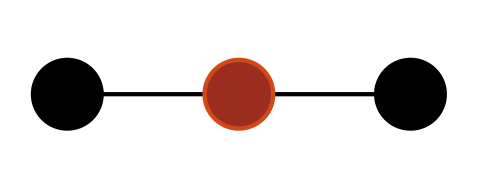
\includegraphics[scale=0.15]{../assets/h_tree_3.png}\end{tabular} & \quad & \begin{tabular}{c}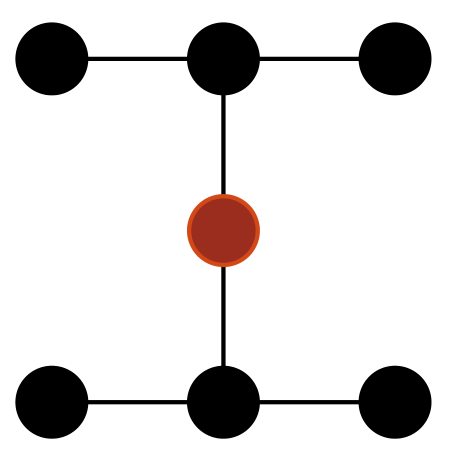
\includegraphics[scale=0.15]{../assets/h_tree_7.png}\end{tabular}
            \end{tabular}
            \caption{Cases for $h = 0$, $h = 1$ and $h = 2$.}
        \end{figure}
        Let $l_h$ and $w_h$ be the two sides of the rectangle enclosing the H tree of height $h$, respectively; thus, we have that
        
        \begin{itemize}
            \item for $h = 0$, $l_0 = w_0 = 2 \implies A_0 = l_0 \cdot w_0 = 2 \cdot 2 = 4 = 2(1+1)$ 
            \item for $h = 1$, $l_1 = 2$ and $w_1 = 4$, therefore $$A_1 = l_1 \cdot w_1 = 2 \cdot 4 = 8 = 2(3+1)$$
            \item for $h = 2$, $l_2 = w_2 = 4 \implies A_2 = l_2 \cdot w_2 = 4 \cdot 4 = 16 = 2(7+1)$
        \end{itemize}
    }{
        Assume the result is true for an H tree of height $h - 1$.
    }{
        Two different cases must be analyzed, specifically when $h$ is \tit{odd} an $h$ is \tit{even}.
        
        \begin{itemize}
            \item For the \tit{odd} case, the sides of the rectangle are defined as follows: $$\soe{l}{l_h = l_{h - 1} = 2l_{h - 2} \\ w_h = 2w_{h - 1} = 2w_{h - 2}}$$ (note that $l_{h - 1} = 2l_{h - 2}$ and $w_{h - 1} = w_{h - 2}$). Therefore
                \begin{equation*}
                    \begin{split}
                        l_h &= 2l_{h-2} \\
                            &= \ldots \\
                            &= 2^k \cdot l_{h - 2k} \quad \quad \rbk{h - 2k = 1 \implies k = \frac{h - 1}{2}} \\
                            &= 2^\frac{h - 1}{2} \cdot l_1 \\
                            &= 2^\frac{h - 1}{2} \cdot 2 \\
                            &= 2^{\frac{h - 1}{2} + 1} \\
                            &= 2^\frac{h + 1}{2}
                    \end{split}
                \end{equation*}
                and analogously
                \begin{equation*}
                    \begin{split}
                        w_h &= 2w_{h - 2} \\
                            &= \ldots \\
                            &= 2^k \cdot w_{h - 2k} \quad \quad \rbk{h - 2k = 1 \implies k = \frac{h - 1}{2}} \\
                            &= 2^\frac{h - 1}{2} \cdot w_1 \\
                            &= 2^\frac{h - 1}{2} \cdot 4 \\
                            &= 2^{\frac{h - 1}{2} + 2} \\
                            &= 2^\frac{h + 3}{2}
                    \end{split}
                \end{equation*}
                Hence, the area is
                \begin{equation*}
                    \begin{split}
                        A_h &= l_h \cdot w_h \\
                            &= 2^\frac{h + 1}{2} \cdot 2^\frac{h + 3}{2} \\
                            &= 2^\frac{2h + 4}{2} \\
                            &= 2^{h + 2} \quad \quad (h = \log (n + 1) - 1) \\
                            &= 2^{\log(n + 1) -1 +2} \\
                            &= 2^{\log(n + 1) +1} \\
                            &= 2(n + 1)
                    \end{split}
                \end{equation*}
            \item For the \tit{even} case, the sides of the rectangle are defined as follows: $$\soe{l}{l_h = 2l_{h - 1} = 2l_{h - 2} \\ w_h = w_{h - 1} = 2w_{h - 2}}$$ (note that $l_{h - 1} = l_{h - 2}$ and $w_{h - 1} = 2w_{h - 2}$) Therefore, the calculations are analogous, but $h - 2k = 0 \implies k = \dfrac{h}{2}$ which leads to $$l_h = w_h = 2^\frac{h + 2}{2}$$ (recall that $l_0 = w_0 = 2$), hence
                \begin{equation*}
                    \begin{split}
                        A_h &= l_h \cdot w_h \\
                            &= 2^\frac{h + 2}{2} \cdot 2^\frac{h + 2}{2} \\
                            &= 2^\frac{2h + 4}{2} \\
                            &= 2^{h + 2} \\
                            &= \ldots \\
                            &= 2(n + 1)
                    \end{split}
                \end{equation*}
        \end{itemize}
    }

    \subsection{The collinear layout}

    The Thompson's Model imposes the restriction that each \tit{processing element} (i.e. node) can have at most \tbf{4 wires} coming out of it in 2D (and 6 in 3D). This constraint ensures that nodes have \textit{manageable connectivity}, which is crucial for simplifying VLSI layouts.

    However, when nodes with \tbf{higher degrees} are \textit{required}, especially in more complex designs, this limitation becomes problematic. By the late 1990s, researchers proposed the following \tbf{non-constant node degree model} as a solution:

    \begin{itemize}
        \item a node with degree $d$ occupies a square with side length proportional to $\Theta(d)$;
        \item the wires connecting these nodes follow \tbf{horizontal or vertical paths} along \tit{grid lines}, similar to how connections are handled in lower-degree models.
    \end{itemize}

    This adaptation maintains simplicity while accommodating \tit{more complex topologies}. This evolution in layout strategies allows for more scalable VLSI design, making it possible to handle larger, more interconnected networks without overly restrictive node degree constraints.

    In particular, this section will focus on a layout proposed by \textcite{yeh}, called the \tbf{collinear layout}, in which all the nodes of the network are placed \tit{on the same line}.

    The following example will show how to get a \tit{collinear layout} from a \tbf{complete graph}.

    \begin{example}[Collinear layouts]
        Consider the following \tit{labeled complete graph}

        \centeredimage[A 6-clique.]{0.2}{../assets/complete_graph.png}

        and let a \tbf{link of type-$i$} be any edge between two nodes whose labels differ by exactly $i$. To obtain the corresponding \tit{collinear layout}, place the 6 nodes on the same line in order, and connect them by placing type-$i$ links in the least possible number of \tbf{tracks} --- in this context a \tit{track} is a horizontal line on which links can be placed. For instance, type-1 links can be placed in 1 track, type-2 links can be placed in 2 tracks --- by placing links between odd numbers on one track and links connecting even numbers on the other --- and so on.

        \centeredimage[Arrangement of links in tracks]{0.2}{../assets/collinear_clique.png}
    \end{example}

    This example shows that type-$i$ links of a collinear layout occupy at most $\min(i, n - i)$. Thus, the total number of tracks of this layout can be obtained by evaluating the following sum:
    
    \begin{equation*}
        \begin{split}
            \sum_{i = 1}^{n - 1}{\min(i, n - i)} &= \sum_{i = 1}^{\frac{n}{2}}{i} + \sum_{i = \frac{n}{2} + 1}^{n - 1}{(n - i)} \\
                                                 &= \sum_{i = 1}^\frac{n}{2}{i} + \sum_{j = 1}^{\frac{n}{2} - 1}{j} \quad \quad (j = n - i) \\
                                                 &= \dfrac{1}{2}\sbk{\dfrac{n}{2} \rbk{\dfrac{n}{2} + 1} + \dfrac{n}{2}\rbk{\dfrac{n}{2} - 1}} \\
                                                 &= \dfrac{n^2}{4}
        \end{split}
    \end{equation*}

    placeholder \todo{incomplete}

    \begin{framedthm}{Thompson's theorem}
        Given a VLSI design, and its corresponding graph $G$, the area occupied by the wires and the nodes of the design is at least $\frac{w^2}{4}$, where $w$ is $G$'s bisection width.
    \end{framedthm}

    \begin{proof}
        The bound of the area of the VLSI design will be proved by counting the minimum number of occupied squares of the grid.

        Consider the VLSI design on a grid as a Cartesian plane, and vertical lines of the form $x = a$. Each possible $x = a$ split the vertices of the network into three separate subsets:

        \begin{itemize}
            \item $L$, which contains the vertices on the left of the vertical line
            \item $R$, which contains the vertices on the right of the vertical line
            \item $S$, which contains the vertices that lie right on the vertical line
        \end{itemize}

        In particular, by monotonicity, there exists an $a$ such that $\abs L + \abs S \ge \dfrac{n}{2}$ and $\abs R + \abs S \ge \dfrac{n}{2}$. Clearly, if $\abs S = 0$, the line $x = a$ cuts the graph into two sets of vertices $L$ and $R$, which must cut at least $w$ edges (by definition of \tit{bisection width}). Otherwise, if $\abs S \neq 0$, $S$ can be split into two subsets $S_1$ and $S_2$, such that $\abs {L \cup S_1} = \abs{R \cup S_2} = \frac{n}{2}$, and the vertical line will still cut at least $w$ edges.

        The line $x = a$ is said to account for the $w$ square units of area of wire and vertices that lie within $\frac{1}{2}$ unit distance of it.

        Consider a \curlyquotes{zig-zag} defined as follows: $$Z_1(x) := \soe{ll}{a - 1 & y \ge b_1 \\ a - 1 \le x \le a + 1 & y = b_1 \\ a + 1 & y \le b_1}$$ where $b_1$ is such that $Z_1$ still bisects the graph, therefore it cuts at least $w$ edges. Note that the horizontal segment of $Z_1$ may cut at most 2 wires, therefore its vertical sections will cross at least $w - 2$ wires.

        Consider each possible zig-zag $$Z_k(x) := \soe{ll}{a - k & y \ge b_k \\ a_ k \le x \le a + k & y = b_k \\ a + k & y \le b_k}$$ where $b_k$ is such that $Z_k$ still bisects the graph, therefore it cuts at least $w$ edges. Since the horizontal segment will cut $2k$ edges, the vertical sections of $Z_k$ will cut $w - 2k$ edges.

        Finally, since $\floor{\dfrac{w}{2}}$ zig-zags can be drawn on the graph (by definition of \tit{bisection width}), the total area of wire and vertices of the VLSI design is at least $$\sum_{k = 0}^{\floor{\frac{w}{2}}} > \dfrac{w^2}{4}$$
    \end{proof}

    \subsection{The Wise layout} \label{wise}

    In a paper published by \textcite{butterwise}, it was proposed a \tit{different layout} for the butterfly network (discussed in \cref{butterfly_networks}), which is shown in the following figure.

    \centeredimage[The alternative layout of the butterfly network.]{0.3}{../assets/butterwise.png}

    Note that inputs are placed in the upper layer, and outputs in the lower layer; also, the \tit{blue circles} represent nodes of the butterfly network, and \tit{black squares} represent \tbf{devices} that allows to avoid interference, since those wire conjunctions are \tit{knock-knees}.

    \centeredimage[Rearrangement to get the Wise layout.]{0.2}{../assets/butterwise_perm.png}

    This rearrangement of the wires allows to have some important \tit{properties}.
    
    \begin{itemize}
        \item All the wires in the same layer have \tbf{equal length}. Note that this is \tit{not true} for every layout; for instance, in the \tit{classical drawing} of the butterfly network, the \tit{straight edges} in the last layer have \tbf{unit length}, while the \tit{cross-edges} in the same layer have lengths that \tbf{scale} linearly with the input size $N$. This disparity is problematic, as it causes a \tit{loss of synchronization} in the information flow. Nevertheless, this length grows exponentially.
        \item The length of the \tbf{longest path} from any input to any output is linear in $N$, namely $2(N - 1)$, and it can be computed by evaluating the diagonal of the square having side length equal to $\sqrt 2 (N - 1)$, shown in figure \todo{add pic}
            which is$$\sqrt{2 \cdot \rbk{\sqrt{2}(N - 1)}^2} = \sqrt{2 \cdot 2 \rbk{N - 1}^2} = \sqrt{4 \cdot \rbk{N - 1}^2} = 2( N - 1)$$
        \item placeholder \todo{pag 20 slide?}
        \item The value of the \tbf{area} of this layout is good, which is $$\rbk{\sqrt 2(N - 1)}^2 = 2N^2 + o(N^2)$$
    \end{itemize}

    Later studies found that the \tbf{area} of this layout is \tit{inaccurate} because the \tbf{slanted} lines --- rotated by 45° --- that define this layout cannot be produced by machines of the fabrication process. In fact, machines can only create \tit{horizontal and vertical lines}, which means that the actual layout on a board would occupy significantly more area.

    \centeredimage[The \tit{actual} Wise butterfly layout.]{0.2}{../assets/rotated_butterwise.png}

    The area of this layout can be evaluated by calculating the area of this \tit{bigger} square, which has side length $2(N - 1)$: $$\rbk{2(N -1)}^2 = 4N^2 + o(N^2)$$ Additionally, \tit{knock-knees} are not avoided, but arranged in the layout thanks to devices that enlarge the layout area even more.

    \subsection{Layered layout}

    In 2000 \textcite{seven} presented a new layout, based on the \tbf{layered cross product} between graphs, which is described below.

    \begin{frameddefn}{Layered graph}
        A \tbf{layered graph} of $l + 1$ layers $G = (V_0, \ldots, V_l, E)$ consists of $l + 1$ layers of nodes, where $V_i$ is the $i$-th node layer, and each edge $(u, v) \in E$ connects $u$ and $v$ if and only if $u \in V_i$ and $v \in V_{i + 1}$ --- i.e. they belong to adjacent layers.
    \end{frameddefn}

    \begin{example}[Layered graphs]
        The following is an example of a layered graph.

        placeholder \todo{add pic}
    \end{example}

    \begin{frameddefn}{Layered cross product}
        Given two layered graphs $G_1 = (V_0^1, \ldots, V_l^1, E^1)$ and $G_2 = (V_0^2, \ldots, V_l^2, E^2)$ of $l + 1$ layers, the \tbf{layered cross product} (LCP) is a new \tit{layered graph} $$G = G_1 \times G_2 := (V_0, \ldots, V_l, E)$$ defined as follows:

        \begin{itemize}
            \item for each $i \in [0, l]$, $V_i := V_i ^1 \times V_i^2$, i.e. each layer in $G$ is the \tit{cartesian product} of the corresponding two layers in $G_1$ and $G_2$;
            \item $((u^1, u^2), (v^1, v^2)) \in E \iff (u^1, u^2) \in E^1 \land (v^1, v^2) \in E_2$, i.e. there is an edge between two nodes of $G$ if and only if the corresponding nodes were connected in the original graphs.
        \end{itemize}
    \end{frameddefn}

    Note that the LCP is not commutative.

    \begin{example}[LCPs]
        The following is an example of an LCP between two graphs.
        
        \centeredimage[An LCP between two graphs.]{0.2}{../assets/lcp.png}
    \end{example}

    LCPs are particularly useful because \textcite{evenlitman} showed that \tit{various topologies} can be defined as LCPs of \tit{simpler structures}, such as trees. Specifically, it can be shown that butterfly networks are LCPs of \tbf{two complete binary trees}, one oriented upward and the other downward.

    \centeredimage[The LCP that defines the 2-dimensional butterfly network.]{0.27}{../assets/butterfly_lcp.png}

    Interestingly, the LCP of two graphs can be evaluated through a method known as \tbf{Projection Methodology} (PM), as illustrated below.

    \centeredimage[The LCP of the two graphs is obtained by this projection.]{0.27}{../assets/lcp_pm.png}

    It is important to note that the PM may produce results that \tit{do not align} with the requirements of the Thompson's Model. For instance, while the projection above still represents the same butterfly network as before, it is not an \tbf{orthogonal drawing}.

    Consider the following projection plane.

    \centeredimage[Possible edge cross products.]{0.2}{../assets/lcp_edges.png}
    
    From these projections, it is evident that:

    \begin{itemize}
        \item the product of \tit{two diagonal edges} yields a \tit{diagonal edge}, which is \tit{not allowed};
        \item the product of a \tit{vertical edge} and a \tit{diagonal edge} yields a \tit{vertical edge}, which is allowed;
        \item the product of a \tit{diagonal edge} and a \tit{vertical edge} yields a \tit{horizontal edge}, which is allowed;
        \item the product of \tit{vertical edges} yields \tit{two overlapping points}, which is \tit{not allowed}.
    \end{itemize}

    Therefore, to achieve a \tit{valid layout} using the PM, it is essential to ensure that the product of \tit{two diagonal edges} or \tit{two vertical edges} \tbf{never occurs}.

    Note that this is not the only problem that may occur in layouts generated through the PM.

    \begin{frameddefn}{Consistent edges}
        Two edges $e_1$ and $e_2$ are said to be \tbf{consistent} if the open intervals of their projections along the same axis are \tit{disjoint}.
    \end{frameddefn}

    \begin{example}[Consistent edges]
        Consider the following edges and their projections on the $x$-axis:

        \centeredimage[Consistent and inconsistent pair of edges, from left to right.]{0.3}{../assets/intervals.png}

        The first two edges are \tit{consistent}, while the other two are not.
    \end{example}

    \tit{Consistency} of edges in the input graphs must be checked, to avoid overlapping wires in the resulting graph. In particular, \tit{two cases} must be avoided.

        In this first scenario, in $G_1$ there are two inconsistent edges in the same layer $i$, and there is an edge in $G_2$ in layer $i$ as well. This produces two overlapping edges in the projection.

        \centeredimage[First inconsistency case]{0.25}{../assets/consistency1.png}

        Note that this situation arises only when the edge in $G_2$ is parallel to the $x$-axis, as it cannot be drawn diagonally, since the inconsistent edges in $G_1$ are already diagonal, and ---  as previously discussed --- the cross product between two diagonal edges must be avoided.

        The second scenario occurs when in $G_1$ there are two inconsistent edges in different layers $i_1$ and $i_2$, and there are collinear edges in $G_2$ in layers $i_1$ and $i_2$ as well. This produces two overlapping edges in the projection.

        \centeredimage[Second inconsistency case]{0.3}{../assets/consistency2.png}

    All the required constraints are summarized in the next proposition.

    \begin{framedprop}{Valid PM layouts}
        Given two graphs $G_1$ and $G_2$, the PM between them generates \tbf{valid layouts}, i.e. in the resulting graph

        \begin{enumerate}
            \item every edge lies on grid lines
            \item at most one node is mapped to each grid point
            \item no pair of edges overlap
        \end{enumerate}
        
        if and only if

        \begin{enumerate}
            \item the cross product of any pair of edges $e_1 \in E_1$ and $e_2 \in E_2$ is such that exactly one between $e_1$ and $e_2$ is drawn diagonally
            \item for each $i \in [0, l]$, it holds that $$\bigcap_{i = 0}^l{\{\abk{u_x,v_z} \mid u \in V_i^1, v \in V_i^2 \}} = \varnothing$$ where $\abk{u_x, v_z}$ is the node at the intersection of the projection lines of $u$ and $v$ along the $x$ ans $z$ axes, respectively
            \item there are no edges in $G_2$ on layers that contain inconsistent edges in $G_1$, and no collinear edges in different layers of $G_2$ in which $G_1$ has inconsistent edges
        \end{enumerate}

        respectively.

    \end{framedprop}

    For the first constraint, a solution is to \tbf{double} the number of layers, such that the edges in the drawing of $G_1$ are diagonal in \tit{odd} layers, and straight in the \tit{even} layers, while the edges in the drawing of $G_2$ are straight in the \tit{odd} layers, and diagonal in the \tit{even} layers.

    \centeredimage[A complete layered binary tree with the nodes doubled.]{0.3}{../assets/doubled.png}

    The second constraint can be addressed by ensuring that no pair of nodes in the drawing of the first (or second) graph, except for the two endpoints of the same straight edge, share the same $x$-coordinate (or $z$-coordinate). This is always achievable by appropriately enlarging the drawings of the two graphs.
    
    Lastly, the third constraint is more difficult to enforce and presents a significant limitation of this technique. For this reason, the focus of this work is restricted to networks where each LCP is calculated from two complete layered binary trees, with double the number of nodes.

    \centeredimage[The LCP of two such trees.]{0.3}{../assets/square_butterfly.png}

    This figure represents the \tbf{planar layout} of a butterfly network, which adheres to all the previously outlined constraints. Moreover

    \begin{itemize}
        \item it is symmetric;
        \item it is a square with side length $2(N - 1)$, therefore the area is $4N^2 + o(N^2)$ --- note that this area is worse than the Wise layout (discussed in \cref{wise}) because in this case the whole area is filled, whereas the Wise layout only uses a portion of such a big area;
        \item all the edges on the same layer have the same length;
        \item unfortunately, input and output nodes do not lie on the boundaries.
    \end{itemize}

    \subsection{Optimal area of the butterfly network}

    \begin{framedlem}{}
        Given an $n$-dimensional butterfly network, for any non-negative integers $j, k > 0$ such that $0 \le j \le j + k \le n$, the subgraph of the butterfly network induces by the nodes in levels $j, j + 1, \ldots, j + k$ is the disjoint union of $2^{n - k}$ copies of $k$-dimensional butterfly networks.
    \end{framedlem}

    In particular, if $j = 0$ and $k = n - 1$, we get have the following \todo{add pic}

    Therefore, an $(n - 1)$-dimensional butterfly network can be built from a pair of $(n - 2)$-dimensional butterfly networks connected by one node layer and one ege layer. \todo{what?}

    \chapter{The worm propagation prevention problem}

    A \href{https://en.wikipedia.org/wiki/Computer_worm}{computer worm} is a type of malware designed to self-replicate and spread across networks without needing a host program. Unlike \tit{viruses}, which require human action to propagate, \tbf{worms} use computer networks to exploit security vulnerabilities in target systems, infiltrating and duplicating themselves automatically.

    Once a worm gains access, it can spread rapidly to other devices, causing network slowdowns, data breaches, or system damage, depending on the worm's purpose. Additionally, worms can carry payloads that steal sensitive data, install other forms of malware, or create backdoors for unauthorized access. Effective network security measures, such as patching vulnerabilities and monitoring traffic, are essential to prevent worm attacks.

    The harmful effects of a worm can be broadly classified into \tit{two categories}:

    \begin{itemize}
        \item \tbf{Direct damage}. These are caused by the worm's execution on the victim's system. It may lead to system instability, data corruption, file deletion, or even the theft of sensitive information. The worm might consume significant system resources, slowing down performance or rendering the machine unusable. They consist solely of instructions to replicate themselves, and typically do not cause severe direct damage beyond consuming computational resources, which can degrade system performance. However, more advanced \tit{direct damage} worms often disrupt the proper functioning of security software, such as antivirus programs and firewalls, making it harder to detect and remove the malware. This interference can severely hinder the normal operation of the infected machine. In many cases, they also act as \tit{carriers} for the automatic installation of \href{https://en.wikipedia.org/wiki/Backdoor_(computing)}{backdoors} or \href{https://en.wikipedia.org/wiki/Keystroke_logging}{keyloggers}, which can later be exploited by attackers or other forms of malware, further compromising the system's security.
        \item \tbf{Indirect damage}. These arise from the methods the worm uses to spread. For example, worms can generate a large volume of traffic while replicating, which can overwhelm networks, disrupt email systems, and lead to costly downtime or loss of productivity. Additionally, their use of social engineering tactics might result in reputational damage or further security breaches. Their damages result from the widespread infection of many computers across a network, creating cascading effects. These type of worms send numerous email messages during replication, flooding inboxes and contributing to email spam, which wastes valuable bandwidth and user attention. They exploit known vulnerabilities in certain software which can lead to software malfunctions, causing instability in the operating system. This often results in system crashes, forced reboots, or even shutdowns, further disrupting normal operations..
    \end{itemize}

    Assume that the time required to transmit information over any connection in a network is constant and denoted as $T$. If a worm successfully infects a set of nodes $C$, and the worm can spread to all other nodes in the network in a single step, then the entire network will be \tbf{infected} within time $T$. Therefore, we are interested in finding the set of nodes $C$ that can lead to a fully infected network.

    The property that every edge in the network is incident to at least one node in the infected set $C$ ensures that the entire network can be infected after the first propagation step. This condition is \tit{sufficient} (though not \tit{necessary}) to guarantee that the worm will spread to all the nodes in the next step.

    From a network manager's perspective, any filter implemented to protect against first-order worm attacks typically reduces communication efficiency. Therefore, \tbf{minimizing} the number of filters is crucial to strike a balance between security and maintaining communication speed.

    Note that, in reality, the situation is more complicated because large-scale networks tend to have \tit{dynamic connections}, meaning the structure of the network changes over time, which can affect the speed and manner of the worm's propagation.

    \section{The vertex cover problem}

    The problem of finding the set $C$ of vertices discussed earlier, where each edge in the network is incident to at least one vertex in $C$, can be reduced to finding the \tbf{minimum vertex cover} of the network graph.
    
    \begin{frameddefn}{Vertex cover}
        Given a graph $G$, a \tbf{vertex cover} for $G$ is a set of vertices $C \subseteq V(G)$ such that every edge in $G$ is incident to at least one vertex in $C$. Using symbols $$\forall (u, v) \in E(G) \quad u \in C \lor v \in C$$
    \end{frameddefn}

    Note that the minimum vertex cover is not unique. Moreover, for any graph $G$, $V(G)$ is trivially a vertex cover for $G$. To find the minimum vertex cover is not trivial, because there are $\powerset(V(G)) = 2^{V(G)}$ possibile subsets of vertices to check.
    
    \begin{example}[Vertex covers]
        The following are two examples of minimum vertex covers for the given graph: \todo{this is wrong}
        \begin{figure}[H]
            \centering
            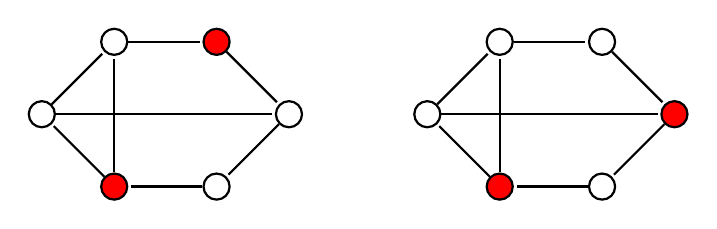
\begin{tikzpicture}[-,>=stealth,shorten >=1pt,auto,node distance=1.3cm, thick,main node/.style={scale=0.9,circle,draw,font=\sffamily\normalsize}]

                \node[circle, draw]  (1) []{};
                \node[circle, draw, fill=red]  (2) [right of = 1]{};
                \node[circle, draw]  (3) [below right of = 2]{};
                \node[circle, draw]  (4) [below left of = 3]{};
                \node[circle, draw, fill=red]  (5) [left of = 4]{};
                \node[circle, draw]  (6) [above left of = 5]{};

                \node[circle, draw]  (1b) [above right of = 3, xshift=50]{};
                \node[circle, draw]  (2b) [right of = 1b]{};
                \node[circle, draw, fill=red]  (3b) [below right of = 2b]{};
                \node[circle, draw]  (4b) [below left of = 3b]{};
                \node[circle, draw, fill=red]  (5b) [left of = 4b]{};
                \node[circle, draw]  (6b) [above left of = 5b]{};

                \path[every node/.style={font=\sffamily\small}]

                (1) edge (2)
                (2) edge (3)
                (3) edge (4)
                (4) edge (5)
                (5) edge (6)
                (6) edge (1)
                (6) edge (3)
                (5) edge (1)

                (1b) edge (2b)
                (2b) edge (3b)
                (3b) edge (4b)
                (4b) edge (5b)
                (5b) edge (6b)
                (6b) edge (1b)
                (6b) edge (3b)
                (5b) edge (1b)
            ;
            \end{tikzpicture}
            \caption{Two minimum vertex covers for a graph.}
        \end{figure}
    \end{example}

    For the reasons mentioned, every minimum vertex cover serves as an excellent starting point for a worm's propagation within a network. Protecting the computers corresponding to the nodes in the \tbf{minimum vertex cover} of the communication graph is crucial. This strategy ensures that every edge in the graph is monitored, thus preventing a worm from exploiting vulnerabilities in unprotected nodes.

    Moreover, if the graph has multiple minimum vertex covers, it is essential to identify and protect \tit{at least} the computers that lie in the \tbf{intersection} of all these covers. This intersection represents the most secure nodes, as they are critical in preventing the spread of the worm across all potential configurations of the network.

    The following definition provides the \tbf{decisional version} of the minimum vertex cover problem.

    \begin{frameddefn}{Minimal Vertex Cover (VC) problem}
        Given a graph $G$, and an integer $k \ge 0$, is there a vertex cover $C$ for $G$ such that $\abs C \le k$?
    \end{frameddefn}

    The VC problem is one of Karp's 21 \NPComplete problems \cite{karp}, which are a collection of well-known computational problems that were classified as \NPComplete shortly after the introduction of the Cook theorem \cite{cook}.

    The VC problem can be also formulated as a 0-1 \tbf{integer linear program} (ILP):
    \begin{itemize}
        \item for every node $v \in V(G)$, we define the variabile $x_v$
        \item for every edge $(i,j) \in E(G)$ we add the constraint $x_i + x_j \geq 1$. This constraint enforces that at least one between $x_i$ and $x_j$ has to be set to 1
    \end{itemize}

    Therefore, we get the following ILP:

    \[\begin{array}{ccc}
        \qquad\qquad\quad
        & \min \; \sum\limits_{i = 1}^n x_i \\\\
        & x_i + x_j \geq 1 & \forall (i,j) \in E(G) \\
        & x \in \{0,1\}^n
    \end{array}\]

    This formulation is a reduction from VC to ILP, implying that the latter is \NPComplete as well.

    Despite the fact that the VC problem is \NPComplete, it is possible to find an \tit{approximate solution} in polynomial time by leveraging its ILP formulation, by employing an ILP approximated solution.

    \subsection{Approximation algorithms}

    There are multiple algorithms for finding approximated solutions for the VC problem. The first algorithm presented is a naïve solution, based on a \tbf{greedy} approach.

    \begin{framedalgo}[label={alg:first_greedy_avc}]{First greedy AVC}
        Given an undirected graph $G$, the algorithm finds an approximated minimum vertex cover for $G$. \\
        \hrule

        \quad
        \begin{algorithmic}[1]
            \Function{firstGreedyAVC}{$G$}
                \State $V' := \varnothing$
                \State $E' := E(G)$
                \While{$E' \neq \varnothing$}
                    \State Choose $(i, j) \in E'$
                    \State $V' = V' \cup \{i\}$
                    \For{$(i, k) \in E(G)$} \Comment{any edge having $i$ as an endpoint}
                        \State $E' = E' - \{(i, k)\}$
                    \EndFor
                \EndWhile
                \State \tbf{return} $V'$
            \EndFunction
        \end{algorithmic}
    \end{framedalgo}

    \idea{
        At each iteration of the algorithm, an edge $(i, j ) \in E'$ is chosen randomly, then $i$ is added to the vertex cover set $V'$, and any edge having $i$ as an endpoint is removed from $E'$. This ensures that $V'$ is a vertex cover, though it may not be minimum.
    }

    \cost{
        Each edge has to be either explored or removed by the algorithm, therefore the cost is $O(n + m)$.
    }

    Consider a graph formed by two rows of nodes as follows: the upper row has $r$ nodes, and the lower row has $k > r$ nodes. Each node of the upper row is connected to each node on the lower row. Note that the upper row is a \tit{minimum} vertex cover for the graph.

    Suppose that the algorithm always chooses the nodes from the lower row, then the resulting set of nodes is a vertex cover made of $k$ nodes. Thus, the approximation ratio between this set of nodes and the minimum vertex cover is $$\dfrac{k}{r} = \dfrac{n - r}{r}$$
   
    \begin{framedalgo}{Second greedy AVC}
        Given an undirected graph $G$, the algorithm finds an approximated minimum vertex cover for $G$. \\
        \hrule

        \quad
        \label{alg:second_greedy_avc}
        \begin{algorithmic}[1]
            \Function{secondGreedyAVC}{$G$}
                \State $V' := \varnothing$
                \While{$E(G) \neq \varnothing$}
                    \State $v \in \argmax_{v \in V(G)}{\deg(v)}$
                    \State $V' = V' \cup \{v\}$
                    \For{$(u, v) \in E(G)$} \Comment{any edge having $v$ as an endpoint}
                        \State $G\texttt{.remove\_edge(}u, v\texttt{)}$
                    \EndFor
                \EndWhile
                \State \tbf{return} $V'$
            \EndFunction
        \end{algorithmic}
    \end{framedalgo}

    \idea{
        At each step of the algorithm, the vertex with the highest degree $v$ is choosen from the current set of vertices $V(G)$, then $v$ is added to the vertex cover $V'$, and any edge having $v$ as an endpoint is removed from $G$. This ensures that $V'$ is a vertex cover, though it may not be minimum.
    }

    \cost{
        At each iteration, the cost of finding $v$ is $O(m)$, and because the cost of removing an edge from $G$ is $O(n + m)$, we have that the cost of the algorithm is $O(m (n + m))$.
    }

    Note that algorithm can produce a vertex cover $V'$ whose cardinality is \tit{vary far} from optimum. In fact, consider the following graph: \todo{add pic}

    The upper row of nodes consists of $r$ nodes, and the lower row consists of

    \begin{itemize}
        \item $r$ nodes of degree 1
        \item $\floor{\dfrac{r}{2}}$ nodes of degree 2 $\ldots$
        \item in general, $\floor{\dfrac{r}{i}}$ nodes of degree $i$
    \end{itemize}

    meaning that the total number of nodes is $$n = r + \sum_{i = 1}^r{\floor{\dfrac{r}{i}}} \le r + r \sum_{i = 1} ^r{\dfrac{1}{i}} = \Theta(r \log r)$$ (note that the \href{https://en.wikipedia.org/wiki/Harmonic_series_(mathematics)}{harmonic sum} can be approximated by $\Theta(\log r)$). Although the \tbf{optimal} minimum vertex cover is the \tit{upper row} itself, consisting of $r$ nodes, it may happen that the algorithm chooses the \tit{lower row} as vertex cover, as shown in the following figure \todo{add pic}

    This means that there is an approximation ratio of $$\dfrac{\Theta(r \log r)}{r} = \Theta(\log r)$$

    However, there are better algorithms that can find approximated minimum covers $V'$ for a given graph $G$ such that $\abs{V'} \le 2 \abs {V^*}$, where $V^*$ is a minimum vertex cover.

    \begin{framedalgo}{2-approximation VC}
        Given an undirected graph $G$, the algorithm finds an approximated minimum vertex cover $V'$ for $G$, such that $\abs{V'} \le 2 \abs {V^*}$, where $V^*$ is a minimum vertex cover. \\
        \hrule

        \quad
        \label{alg:2-approx_vc}
        \begin{algorithmic}[1]
            \Function{2approxVC}{$G$}
                \State $V' := \varnothing$
                \State $E' := E(G)$
                \While{$E' \neq \varnothing$}
                    \State Choose $(i, j) \in E'$
                    \State $V' = V' \cup \{i, j\}$
                    \For{$(i, k) \in E(G)$} \Comment{any edge having $i$ as an endpoint}
                        \State $E' = E' - \{(i, k) \}$
                    \EndFor
                    \For{$(j, h) \in E(G)$} \Comment{any edge having $j$ as an endpoint}
                        \State $E' = E' - \{(j, h) \}$
                    \EndFor
                \EndWhile
                \State \tbf{return} $V'$
            \EndFunction
        \end{algorithmic}
    \end{framedalgo}

    \idea{
        The algorithm computes as the \cref{alg:first_greedy_avc}, but both endpoint of the choosen edge are considered in the removal step.
    }

    \cost{
        The cost of the algorithm is the same of the \cref{alg:first_greedy_avc}, which is $O(m(n +m))$.
    }

    \begin{proof}
        We will prove that any $V'$ returned from the algorithm is such that $\abs{V'} \le 2 \abs {V^*}$ for some minimum vertex cover $V^*$. Note that, by construction, $V'$ is a vertex cover for $G$.

        Let $A$ be the set of the edges \tit{choosen} from $E'$. For each edge $(i, j) \in A$, $i$ and $j$ are added to $V'$ by the algorithm, therefore $$\abs{V'} = 2 \abs A$$

        Moreover, all the edges having either $i$ or $j$ as endpoint are removed from $E'$, thus edges in $A$ cannot be incident, which means that there exists a minimum vertex cover $V^*$ such that $$\abs A \le \abs{V^*}$$

        Finally, we have that $$\abs{V'} = 2 \abs A \le 2 \abs{V^*}$$
    \end{proof}

    \begin{framedalgo}{2-approximation VC (ILP)}
        Given an undirected graph $G$, the algorithm returns a vector that represents an approximated minimum vertex cover $V'$ for $G$, such that $\abs{V'} \le 2 \abs {V^*}$, where $V^*$ is a minimum vertex cover. \\
        \hrule

        \quad
        \label{alg:2-approx_vc_ilp}
        \begin{algorithmic}[1]
            \Function{2approxVCilp}{$G$}
                \State Consider the ILP formulation of the VC problem on $G$
                \State Relax the ILP by replacing the $x \in \{0, 1\}^n$ constraint into $x \in [0, 1]^n \subseteq \R^n$
                \State $x^* := \texttt{polyLPSolver()}$
                \State $y^* \in \{0, 1\}^n$
                \For{$i \in [1, n]$}
                    \If{$x_i \ge \frac{1}{2}$}
                        \State $y_i^* := 1$
                    \Else
                        \State $y_i^* := 0$
                    \EndIf
                \EndFor
                \State \tbf{return} $y^*$
            \EndFunction
        \end{algorithmic}
    \end{framedalgo}

    \idea{
        By relaxing the ILP formulation of the VC problem on $G$ to a LP problem, we can use any polynomial LP solver to get a fractional solution $x^* \in [0, 1]^n$. Thus, to get a valid vertex cover, it is sufficient to consider only the $x^*_i$'s such that $x^*_i \ge \frac{1}{2}$.
    }

    \begin{proof}
        Let $V'$ be the set of vertices described by $y^*$. It is easy to see that $V'$ is a vertex cover for $G$, because the constraint of the ILP $$x^*_i + x^*_j \ge 1$$ forces at least one between $x^*_i$ and $x^*_j$ to be greater or equal than $\frac{1}{2}$, therefore at least one between $y^*_i$ and $y_j^*$ will be set to 1.

        Now we will prove that the algorithm returns a 2-approximation of an optimal solution $V^*$. Let $$Z := \sum_{i = 1}^n{x^*_i}$$ Since $x^*_i \le 1$ for each $i \in [1, n]$, it must be that $Z \le \abs{V^*}$ \todo{what?}. Let $y^* \in \{0, 1\}^n$ be the integer solution obtained from $x^* \in [0, 1]^n$ by the rounding procedure; clearly, for each $i \in [1, n]$, we have that $y^*_i \le 2x^*_i$, therefore $$\abs{V'} = y^*_1 + \ldots + y^*_n \le 2 (x^*_1 + \ldots + x^*_n) = 2Z \le 2 \abs{V^*}$$
    \end{proof}

    The vertex cover problem is related to many other graph theory problems.

    \begin{frameddefn}{Independent set}
        Given an undirected graph $G$, $S \subseteq V(G)$ is an \tbf{independent set} if and only if $$\forall v, v' \in S \quad \nexists (v, v') \in E(G)$$
    \end{frameddefn}

    \begin{framedthm}{}
        A set of nodes $V'$ is a vertex cover over a graph $G$ if and only if its complement $V(G) - V'$ is an independent set.
    \end{framedthm}

    \proofiff{
        By way of contradiction, assume that there exist $x, y \in V(G) - V'$ such that $(x, y) \in E(G)$; note that neither $x$ nor $y$ are in $V'$ because they are in its complement, therefore $(x, y)$ is not covered by the vertex cover $V'$.
    }{
        Analogously, by way of contradiction, assume that there exists an edge $(x, y) \in E(G)$ that is not covered by any node in $V'$, then both $x, y \in V(G) - V'$, therefore there exist two adjacent nodes in $V(G) - V'$.
    }

    \begin{framedcor}{}
        The number of nodes of a graph is equal to the size of its minimum vertex cover, plus the size of a maximum independent set.
    \end{framedcor}

    \begin{frameddefn}{Matching}
        Given a graph $G$, $M \subseteq E(G)$ is a \tbf{matching} of $G$ if and only if $$\forall (x, y), (u, v) \in M \quad x , y\neq u,v$$
    \end{frameddefn}

    The nodes that are not covered by a matching are called \tbf{free nodes}.

    \begin{frameddefn}{Perfect matching}
        Given a graph $G$, a \tbf{perfect matching} is a matching that covers every vertex of the $G$.
    \end{frameddefn}

    Note that every perfect matching is a \tit{maximum matching}. Additionally, note that a perfect matching exists only if the number of vertices $n$ of $G$ is even, since each edge of the perfect matching covers exactly 2 vertices. In particular, the cardinality of a perfect matching is always $\frac{n}{2}$, since each node is adjacent to exactly one edge of the perfect matching.

    \begin{framedthm}[label={bounded_matching}]{}
        Let $M$ be a matching of $G$ and $C$ a vertex cover for $G$; then $\abs M \le \abs C$.
    \end{framedthm}

    \begin{proof}
        $C$ is a vertex cover, thus it must cover all edges in $E(G)$, and in particular it covers all edges in $M$. By definition of vertex cover, for each edge in $M$, at least one of its endpoints must be in $C$, therefore $\abs C$ must be at least $\abs M$.
    \end{proof}

    \begin{framedcor}{}
        Let $M$ be a matching of $G$ and $C$ a vertex cover for $G$. If $\abs M = \abs C$ then $M$ is a maximum matching and $C$ is a minimum vertex cover.
    \end{framedcor}

    Note that, although a maximum matching can be found in polynomial time, the contrapositive of this corollary is not true in general, therefore it is not possible to try to solve the minimum vertex cover through the maximum matching problem.

    \begin{framedalgo}{2-approximation VC (matching)}
        Given an undirected graph $G$, the algorithm returns a minimum vertex cover $V'$ for $G$, such that $\abs{V'} \le 2 \abs {V^*}$, where $V^*$ is a minimum vertex cover. \\
        \hrule

        \quad
        \label{alg:2-approx_vc_matching}
        \begin{algorithmic}[1]
            \Function{2approxVCmatching}{$G$}
                \State $M := \texttt{findMaximalMatching(}G\texttt{)}$
                \State $V' := \varnothing$
                \For{$(u, v) \in M$}
                    \State $V' = V' \cup \{u, v\}$
                \EndFor
                \State \tbf{return} $V'$
            \EndFunction
        \end{algorithmic}
    \end{framedalgo}

    \idea{
        By computing a maximum matching $M$ on $G$, all the endpoints of the edges in $M$ will form a vertex cover for $G$, by definition of matching.
    }

    \cost{
        Note that the time complexity of the algorithm depends directly on the algorithm used to compute the maximum matching $M$ of $G$.
    }

    \begin{proof}
        Consider an edge $(u, v) \in E(G)$; this edge is either in $M$, and therefore both endpoints are inserted into $V'$ by the algorithm, or $(u, v) \in E(G) - M$, but at least one of its endpoints must be in $V'$, otherwise it could have been put into $M$, but this is not possible because $M$ is maximum. This proves that $V'$ is a vertex cover.

        Let $V^*$ be a minimum vertex cover for $G$; to prove that $V'$ is a 2-approximation of the VC problem, note that by \cref{bounded_matching} we have that $\abs M \le \abs{V^*}$, therefore $$\abs{V'} = 2 \abs M \le 2 \abs{V^*}$$
    \end{proof}

    \begin{frameddefn}{Bipartite graph}
        A graph $G$ is said to be \tbf{bipartite} if and only if there is a partition $U, W$ of $V(G)$ such that both $U$ and $V$ are independent sets.
    \end{frameddefn}

    Bipartite graphs are very important, because the following theorem, proved by König \cite{konig}, allows to compute a maximum VC on bipartite graphs in polynomial time.

    \begin{framedthm}{König's theorem}
        In any bipartite graph, the number of edges in a maximum matching is equal to the number of vertices in a minimum vertex cover.
    \end{framedthm}

    \subsection{The eternal vertex cover problem}

    In \tbf{Dynamic network security}, the \tit{fault-tolerance model}'s objective is to deploy a \tit{minimum} set of guards across network nodes to provide continuous protection against attacks or faults on any single network link at any time. When an attack or fault occurs on a link, a guard stationed at one of the adjacent nodes detects it and \tit{immediately} moves across the link to defend or repair the issue. Meanwhile, the remaining guards reconfigure by repositioning themselves to adjacent nodes. This reconfiguration ensures that the system remains \tbf{protected} from future attacks or failures, maintaining a dynamic, adaptive defense mechanism.

    This process ensures that protection is not only \tit{instantaneous} but can be maintained \tit{indefinitely}. The guards adjust their positions in response to each new incident, guaranteeing continuous defense against single-link attacks or failures in an \tit{ad infinitum} manner, adapting dynamically to evolving threats or faults without compromising the network's resilience.

    This model can be translated into the \tbf{eternal vertex cover} problem, in which

    \begin{itemize}
        \item the network is modeled as a graph
        \item at most one defender is located at each node
        \item an attacker can target edges
        \item a defender \tit{can} protect all the edges incident to the nodes where the guard is located
        \item to defend an attacked edge, a guard must move along the attacked edge
        \item any guard can traverse one edge at a time
    \end{itemize}

    Given the set of nodes where guards are deployed at any moment, if these nodes do not form a \tbf{vertex cover}, the attacker can exploit any uncovered edge to bypass the defense and successfully breach the network. Therefore, to ensure continuous protection, the defender must \tit{dynamically reconfigure} the guard positions so that the current set of guarded nodes always forms a valid vertex cover. This reconfiguration is crucial after any attack, transforming \tit{one vertex cover into another} in response to the attack, ensuring that no edge remains exposed.

    If $\alpha (G)$ is the cardinality of a minimum VC on a graph $G$, and $\alpha ^{\infty}(G)$ is the cardinality of a minimum eternal VC, then $$\alpha(G) \le \alpha^{\infty}(G)$$

    \begin{framedthm}{Shadow guard}
        Let $G$ be a connected graph, and let $V'$ be a vertex cover for $G$ that induces a connected subgraph of $G$. Then $\alpha^{\infty}(G) \le \abs{V'} + 1$.
    \end{framedthm}

    \begin{proof}
        Choose a vertex $d \in V(G) - V'$, and place a new guard on it; we will refer to this guard as \tit{shadow guard}. Let $P$ be the following path $$P = d, v_1, \ldots, v_k, x$$ where $v_1, \ldots, v_k \in V'$, and $(v_k, x)$ is the attacked edge. To defend $(v_k, x)$, it is sufficient to slide each guard over $P$, towards $x$, therefore the \tit{shadow guard} will now be on $v_1$, and the attacked edge will be defended by the guard that slid from $v_k$ to $x$.

        Finally, note that the new set of vertices on which the guards now stand on still form a vertex cover, hence $V' \cup \{d\}$ is an eternal vertex cover.
    \end{proof}

    \begin{framedlem}{}
        Let $G$ be a connected graph, and let $V'$ be a vertex cover inducing a subgraph of $G$, with $k$ connected components. Then $\alpha^{\infty}(G) \le \abs{V'} + k$.
    \end{framedlem}

    \begin{proof}
        Considering each connected component of $V'$ as a separate connected subgraph, we get the result of the lemma, by the same reasoning of the previous theorem.
    \end{proof}

    Note that $V'$ can induce at most $\abs{V'}$ connected components, therefore we get the following theorem.

    \begin{framedthm}{}
        Given a graph $G$, we have that $$\alpha(G) \le \alpha^{\infty} (G) \le 2 \alpha(G)$$
    \end{framedthm}

    \begin{framedthm}{Eternal VC on cycles}
        For any $n \ge 3$, we have that $$\alpha^{\infty}(C_n) = \alpha(C_n) = \ceil{\frac{n}{2}}$$ where $C_n$ is a cycle graph of $n$ nodes.
    \end{framedthm}

    \begin{proof}
        By placing a guard on alternated nodes of the cycle graph $C_n$, we get an eternal vertex cover: if an edge is attacked, it is sufficient to rotate each guard by 1.
    \end{proof}

    \begin{framedthm}{Eternal VC on paths}
        For any $n \ge 1$, we have that $$\alpha^{\infty}(P_n) = n - 1$$ where $P_n$ is a path graph of $n$ nodes.
    \end{framedthm}
    
    \begin{proof}
        Consider a vertex cover of less than $n - 1$ nodes of $P_n$. It is always possible to design an attack strategy such that all the guards form a connected path, therefore an edge will be unprotected because there are less than $n - 1$ guards.
    \end{proof}

    \chapter{The data mule scheduling problem}

    A \tbf{sensor} is a device that detects and responds to specific \tit{environmental inputs}, such as light, heat, motion, moisture, or pressure, among many other physical phenomena. Upon sensing these inputs, the sensor generates an \tit{output signal}, which can either be displayed locally in a human-readable format or transmitted electronically over a network for further analysis or processing. This process allows sensors to play a crucial role in monitoring and interpreting real-world conditions across a wide range of applications.

    \tbf{Sensor networks} are wireless networks made up of numerous small sensors, often low-cost, designed to collect \tit{environmental data}. These networks are rapidly expanding due to their broad range of applications, enabling effective monitoring and data collection for diverse purposes across industries.

    We assume that the type of networks discussed in this chapter are \tbf{fixed}, therefore the sensor cannot change position over time. Moreover, we assume that the sensors need to send all the gathered information to a \tbf{base station}.
    
    From an engineering standpoint, one of the most critical challenges in fixed sensor networks is \tbf{energy management}, for the following reasons:

    \begin{itemize}
        \item Sensor networks are often deployed in remote or inaccessible areas where direct access to power sources is impractical. As a result, sensors typically rely on \tit{batteries}, which are difficult to replace or recharge due to the network's location and density.
        \item Many sensor network applications require \tit{continuous, long-term data collection} over extended periods, often months or even years, which demands \tit{efficient energy use} to prolong network operation without frequent maintenance.
    \end{itemize}

     Addressing this energy constraints is essential for maintaining reliable and cost-effective sensor network functionality in the field. In particular, since sensors remain \tit{stationary} in this setup, \tbf{wireless communication} becomes one of the most energy-intensive operations on each sensor node. To conserve energy, it's critical to \tbf{minimize communication} where possible.

     A possible approach to the problem may be \tbf{multi-hop communication to the base station}, but this solution is less than ideal due to several potential drawbacks:

    \begin{itemize}
        \item \tbf{unstable communication infrastructure}: connections between nodes in a multi-hop setup can be prone to \tit{instability}, especially in changing environments where interference or physical obstructions disrupt communication paths
        \item \tbf{high energy costs with sparse deployment}: in areas where nodes are \tit{sparsely} deployed, the distance to the nearest node or the base station can be considerable, hence nodes must increase their transmission range to maintain connectivity, consuming significantly more energy and reducing overall network lifespan
        \item \tbf{energy depletion in dense networks}: in \tit{densely} packed networks, nodes near the base station bear a heavy communication load, often forwarding data from distant nodes, which can lead to rapid energy depletion for these nodes, creating bottlenecks in the network and reducing its effectiveness over time.
    \end{itemize}

    Another strategy, which is significantly more \tit{energy-efficient}, is to leverage \tbf{mobile data mules}. A \tit{data mule} is a mobile node equipped with:

    \begin{itemize}
        \item \tbf{wireless communication}, enabling data collection from stationary sensor nodes
        \item \tbf{ample storage capacity}, allowing it to store data collected from multiple sensors
    \end{itemize}

    The data mule traverses the sensing area, collecting data as it comes within close range of each sensor node. Later, it returns to the base station to deposit all gathered data.

    There are multiple advantages to this approach.

    \begin{itemize}
        \item \tbf{energy savings for sensor nodes}: each sensor only needs to transmit data over short distances, conserving substantial energy as it eliminates the need for long-range or multi-hop communication; additionally, sensor nodes avoid the energy cost of forwarding data from other nodes, reducing their workload
        \item \tbf{reduced energy constraints for the data mule}: since data mules typically return to the base station to recharge, their energy limitations are less critical than those of stationary sensors, allowing for more flexible and longer collection periods
        \item \tbf{simplified network management}: this approach reduces the need for complex routing among nodes, which minimizes processing demands on sensors and further extends their battery life
    \end{itemize}

    Although data mules offer greater flexibility in sensor networks, it remains important to ensure they traverse sensor nodes in an \tit{optimized manner}. Efficient traversal minimizes the data mule's battery usage, helping to extend its operational life and reducing associated costs.

    To minimize the time required for a data mule to collect data from all sensor nodes, the problem can be framed as a \tbf{scheduling problem}, where each sensor node's communication represents a \tit{job}. The goal is to control both the movement (i.e. \tit{path} and \tit{speed}) of the data mule and its communication schedule with each node, similar to \href{https://en.wikipedia.org/wiki/Optimal_job_scheduling}{job allocation} in classical scheduling problems.

    However, data mule scheduling presents additional complexity due to unique location and time constraints:

    \begin{itemize}
        \item \tbf{location constraints}: each data transfer becomes available only when the mule is within the \tit{wireless communication range} of a node, thus proximity to each node is essential, which imposes spatial constraints that affect when data can be collected
        \item \tbf{time constraints}: given a fixed bandwidth and a continuously moving mule, each node requires a specific \tit{time window} to transmit its data successfully; note that the data mule \tit{cannot stop}, meaning the timing of its arrival and departure relative to each node must be precise to ensure successful data transfer
    \end{itemize}

    To address these constraints, optimization techniques can be applied to schedule the data mule's path and communication windows effectively:

    \begin{itemize}
        \item \tbf{path optimization}: plan a path that \tit{minimizes travel distance}, while ensuring each node is visited within its communication range
        \item \tbf{speed control}: adjust the mule's speed dynamically based on \tit{node density} and \tit{transmission time} needs, allowing it to linger in areas where longer data transfer times are required
        \item \tbf{adaptive scheduling}: incorporate \tit{adaptive scheduling algorithms} to allocate data transfer time based on each node's data volume and communication range requirements
    \end{itemize}

    More specifically, the problem of efficiently managing a data mule's traversal can be broken down into three interrelated subproblems.

    \begin{itemize}
        \item \tbf{Path selection}: This step involves determining the \tit{optimal trajectory} for the data mule within the sensor field. The goal is to ensure that the data mule comes within the \tit{communication range} of each sensor node at least once to collect data effectively. This subproblem can be approached using \tit{shortest-path algorithms} or \tit{traveling salesman-like} methods, ensuring that the mule visits each required location while minimizing travel distance.
        \item \tbf{Speed control}: After selecting the path, the next challenge is to adjust the data mule's \tit{speed} along this trajectory. The mule must stay within each node's \tit{communication range} just long enough to complete data transfer without stopping. This requires fine-tuning speed based on the data volume and bandwidth limitations at each node, allowing efficient data collection while conserving battery life by avoiding unnecessary idling.
        \item \tbf{Job scheduling}: When the data mule is within range of multiple sensors, it needs a strategy to \tit{decide} the sequence of data collection. This scheduling can be framed as a \tit{job allocation problem}, where each sensor's data transfer represents a \tit{job} with specific time intervals during which it can be completed. The task is to allocate time slots for each job to ensure all data is collected in the shortest possible time. This problem closely aligns with classical job scheduling, where the objective is to assign time slots efficiently to maximize throughput and minimize the overall collection time.
    \end{itemize}

    Since the \tbf{speed contro} subproblem is typically handled by engineers, and the \tbf{job scheduling} subproblem falls outside this chapter's scope, our focus here is on the first subproblem, the \tbf{path selection} for the data mule.

    Consider a scenario where sensor nodes operate at \tit{varying sampling rates} (e.g., pollution sensors that adjust to real-time conditions). Each sensor has a \tit{limited buffer} for storing its data until a mobile data mule—serving as a mobile base station—arrives to offload this information. Once the data mule reaches a sensor node, it transfers the collected data to its own storage, freeing up the sensor's buffer for new data. This setup has several practical implications:

    \begin{itemize}
        \item \tbf{varying sampling rates}: sensors sampling data at different rates may fill their buffers at different speeds, impacting the urgency and frequency of data mule visits, in fact sensors with higher sampling rates (e.g., in highly polluted areas) might require more frequent visits to prevent data loss
        \item \tbf{finite buffer constraints}: since each sensor has a limited data storage capacity, efficient scheduling and path planning for the data mule become crucial to avoid data overflow at any sensor, thus path selection must account for these storage limitations and prioritize nodes based on buffer status and sampling frequency
    \end{itemize}

    The problem of scheduling the visits of a mobile data mule to ensure that none of the sensor nodes' buffers overflow can be summarized as the \tbf{Mobile Element Scheduling (MES)} problem. This problem involves planning the optimal sequence and timing of visits by the data mule to collect data from sensor nodes, considering the limited buffer capacity of each sensor node and the varying data collection rates.

    Now, consider the following well-known computational problem.

    \begin{frameddefn}{Traveling Salesman Problem}
        The Traveling Salesman Problem (TSP) is defined as follows: a salesman has to visit a given set of cities, such that his tour ends on the same city on which he started, while minimizing the total length of the trip.
    \end{frameddefn}

    Note that the MES problem differs from the TSP in key ways:
    
    \begin{itemize}
        \item \tbf{objective}: TSP searches for the shortest path visiting each city (i.e. node) exactly once, while in MES a node may need multiple visits due to varying sampling rate and buffer state
        \item \tbf{deadlines}: in TSP the costs are fixed (the total length of the trip) and there are no time constraints, while in MES deadlines dynamically update after each visit, requiring the data mule to adjust its path in real time
    \end{itemize}

    Despite these differences, TSP-based approaches can still be useful for solving MES, particularly in path planning. In fact, TSP can serve as a useful approximation for MES, by considering the optimal route between nodes, and then adjusting that route dynamically to accommodate nodes that require more frequent visits.

    \section{The Traveling Salesman Problem}

    The origins of the TSP are somewhat ambiguous:

    \begin{itemize}
        \item an 1832 handbook for traveling salesmen references the problem, presenting example routes through Germany and Switzerland, though without any mathematical formulation
        \item in the mid-1800s, mathematicians \href{https://en.wikipedia.org/wiki/William_Rowan_Hamilton}{W. R. Hamilton} and \href{https://en.wikipedia.org/wiki/Thomas_Kirkman}{T. Kirkman} introduced the first formal mathematical formulation of the problem
        \item the TSP in its general form was studied in the 1930s, when researchers analyzed the limitations of the brute-force algorithm and noted the non-optimality of simpler heuristics like the nearest neighbour approach
    \end{itemize}

    \begin{frameddefn}{Hamiltonian cycle}
        Given a graph $G = (V,E)$, a \tbf{Hamiltonian cycle} (HC) is a cycle that passes through each node in $V(G)$ exactly once.
    \end{frameddefn}

    It can be proven that determining whether a graph $G$ contains a HC is \NPComplete --- HC will be used interchangeably for \curlyquotes{Hamiltonian cycle} and the associated decision problem. Now, consider the following decisional version of the TSP.

    \begin{frameddefn}{TSP (decisional version)}
        Let $K_n = (V, E)$ be a complete graph having $n$ nodes, $\func{w}{E(G)}{\R^+}$ be a non-negative edge-weight function, and $t \ge 0$; does $K_n$ contain a Hamiltonian cycle with total cost at most $t$?
    \end{frameddefn}

    Note that any complete graph $K_n$ trivially contains a HC, but the problem aims at minimizing the cost of the HC. The following proof shows that the TSP is \NPComplete as well.

    \begin{framedthm}[label={tsp np compl}]{$\mathrm{TSP} \in \NPComplete$}
        The TSP is \NPComplete.
    \end{framedthm}

    \begin{proof}
        It can be easily proved that TSP is in \NPclass: given a complete graph $K_n =(V, E)$, and a walk over $K_n$, it can be checked in polynomial time if the walk is a Hamiltonian cycle, and its total weight is bounded by $t$.

        Now we will prove that TSP is \NPHard, by reducing HC to TSP as follows:

        \begin{itemize}
            \item consider a graph $G = (V, E)$, and construct the complete graph $K_n = (V, E')$, where $E(G) \subseteq E'(K_n)$ and the remaining edges are the ones added to make $K_n$ a complete graph --- note that $n := \abs{V(G)}$
            \item let $t := n$ and define $\func{w}{E'(K_n)}{\R^+}$ as follows: $$\soe{ll}{w(i, j) = 1 & (i, j) \in E(G) \\ w(i, j) = 2 & (i, j) \in E'(K_n) - E(G)}$$
            \item assume that there exists a Hamiltonian cycle $C$ in $G$; by definition of $w$, all edges of $C$ in $K_n$ have weight 1, since they are all in $G$; this shows that if $G$ has a HC, then $K_n$ has a traveling salesman tour of cost $n = t$
            \item conversely, if $K_n$ has a traveling salesman (TS) tour of cost $n$, all edges of the tour necessarily have weight 1, because edges with weight 2 would not minimize the cost; therefore, by definition of $w$, this tour describes a HC in $G$
            \end{itemize}
    \end{proof}

    In 1954 \textcite{dantzig} showed that the TSP can be formulated as an ILP as well:

    \begin{itemize}
        \item given a complete graph $K_n = (V, E)$, and assume that the TS tour is oriented
        \item define variables $x_{ij}$ and $w_{ij}$ for each $(i, j) \in E(G)$
        \item let $x_{ij} = 1$ if and only if the TS tour traverses the oriented edge $(i, j)$
        \item let $w_{ij} = w(i, j)$
    \end{itemize}

    Then, the TSP can be formulated as an ILP as follows:

    \[\begin{array}{ccc}
        \qquad\qquad\quad
        & \min \; \sum\limits_{(i, j) \in E(G)} {w_{ij}x_{ij}} \\\\
        & \sum\limits_{i = 1}^n {x_{ij}} = 1 & \forall j \in V(K_n) \\
        & \sum\limits_{j = 1}^n {x_{ij}} = 1 & \forall i \in V(K_n) \\
        & \sum\limits_{i, j \in S} {x_{ij}} < \abs S & \forall S \subsetneq V(K_n), S \neq \varnothing \\
        & x \in \{0,1\}^n
    \end{array}\]

    The first two constraints force the tour to be Hamiltonian, by imposing that for any vertex $j$ there must be at most 1 incoming edge, and for each vertex $j$ there must be at most 1 outgoing edge. However, this does not imply that the solution of the ILP is a cycle: in fact, without the third constraint, a valid solution could involve multiple unconnected cycles of $G$. Therefore, the last constraint imposes that any \tit{proper subset} of vertices $S$ of $V(K_n)$ must cover a number of edges that is strictly less than the number of vertices of $S$ itself; in fact, this constraint avoids the possibility of forming cycles in the solution because a cycle has the same number of edges and vertices. Note that, in reality, the last constraint hides $\abs{\powerset(V(K_n))} - 2 = 2^n - 2$ constraints, one for each possible \tit{proper subset} $S$ of $V(K_n)$.

    The next theorem shows that, in addition to being \NPComplete, the TSP is also non-approximable, making it an especially challenging problem.

    \begin{framedthm}{Inapproximability of the TSP}
        If there exists a polynomial time algorithm for the TSP with any approximation ratio $r > 1$, then $\Pclass = \NPclass$.
    \end{framedthm}

    \begin{proof}
        Let $G = (V, E)$ be an instance of HC, and construct a complete graph $K_{\abs V} = (V, E')$ starting from $G$ by adding edges; moreover, define $\func{w}{E(K_n)}{\R^+}$ as follows: $$\soe{ll}{w(i, j) = 1 & (i, j) \in E(G) \\ w(i, j) = 2 + (r - 1) n & (i,j) \in E'(K_n) - E(G)}$$ Note that, for the same reasoning applied in the proof of \cref{tsp np compl}, a TS tour with total weight $n$ exists in $K_n$ if and only if $G$ has a HC.

        Assume there exists an $r$-approximation polynomial algorithm $A$ for the TSP; therefore, because the total weight of the TS tour is $n$, $A$ ran on $K_n$ would find a solution $H$ such that $$\sum_{(i, j) \in H} {w(i, j)} \le rn$$ Now, assume that there exists an edge $(\hat i, \hat j)$ in $H$ such that $(\hat i, \hat j) \in E'(K_n) - E(G)$; hence, by definition of $w$, the total weight of $H$ must be at least $$\sum_{(i, j) \in H}{w(i, j)} = (n - 1) \cdot 1  + 2 + (r - 1)n = n - 1 + 2 + rn - n = rn + 1 > rn$$ because $H$ would be a cycle containing $n - 1$ edges from $E(G)$ and 1 edge from $E'(K_n) - E(G)$. Since $A$ is an $r$-approximation algorithm, this implies that any solution $H$ for $A$ must contain only edges inside $G$, otherwise $H$ would not be an $r$-approximation of an optimal solution for the TSP. However, if any of $A$'s solutions $H$ lie entirely in $G$, then $H$ is a HC for $G$ as previously discussed, which means that $A$ can find a HC in $G$ in polynomial time, which would imply that $\Pclass = \NPclass$ because HC is \NPComplete.
    \end{proof}

    \subsection{Special cases for the TSP}

    Despite this result showing that the TSP is not generally approximable, it is still possible to find effective approximation algorithms for certain special cases. Note that, for any set of edges $E$, the following notation will be used $$w(E) := \sum_{(i, j) \in E}{w(i,j)}$$
    
    \begin{framedlem}[label={tsp bound}]{Lower bound on TS tours}
        Given a graph $G$ and a weight function $\func{w}{E(G)}{\R^+}$, the weight of any TS tour on $G$ is at least the weight of any MST of $G$.
    \end{framedlem}

    \begin{proof}
        Consider a graph $G$, an MST $T$ of $G$, and an optimal TS tour $H^*$ on $G$. Clearly, if by removing and edge from $H^*$, we obtain a path $P$, which has weight strictly less than $H^*$'s weight --- note that this is true because $w(i, j) \in \R^+$ for any $(i, j) \in E(G)$. Moreover, note that a path is a special case of a tree, therefore $P$'s weight must be at least $T$'s weight, by definition of MST. Thus, we have that $$w(T) \le w(P) \le w(H^*)$$
    \end{proof}

    Consider the following special case of graphs.

    \begin{frameddefn}{Metric graphs}
        Given a graph $G$, and a weight function $\func{w}{E(G)}{\R^+}$, $G$ is said to be a \tbf{metric graph} if and only if $$\forall u, v, z \in V(G) \quad w(u, z) \le w(u, v) + w(v, z)$$ which means that $w$ satisfies the triangle inequality.
    \end{frameddefn}

    For metric graphs, there exist algorithm that can approximate solutions for the TSP. In particular, the following algorithm leverages the triangle inequality property of $w$ to obtain a 2-approximation for the TSP.

    \begin{framedalgo}{2-approximation TSP}
        Given a complete graph $K_n = (V, E')$, and a weight function $\func{w}{E'(G)}{\R^+}$ such that $K_n$ is a metric graph, the algorithm finds a TS tour $H$ such that $w(H) \le 2w(H^*)$, where $H^*$ is an optimal TS tour. \\
        \hrule

        \quad
        \label{alg:2-approx_tsp}
        \begin{algorithmic}[1]
            \Function{2approxTSP}{$G$, $w$}
                \State Choose $r \in V(K_n)$ randomly
                \State $T := \texttt{findMST}(K_n, r)$ \Comment{find an MST rooted in $r$}
                \State $\texttt L := \texttt{DFSpreorder}(T)$ \Comment{a \tit{preorder} DFS on $T$}
                \State $V := \varnothing$
                \State $\texttt L' := \texttt{[]}$
                \For{$v \in \texttt L$}
                    \If{$v \notin V$}
                        \State $\texttt L'.\texttt{append}(v)$
                        \State $V = V \cup \{v\}$
                    \EndIf
                \EndFor
                \State \textbf{return} \ttt L' \Comment{\texttt L' is \texttt L without repetitions}
            \EndFunction
        \end{algorithmic}
    \end{framedalgo}

    \begin{proof}
        We will prove that any solution $H$ of the algorithm is a 2-approximation of an optimal solution $H^*$ for the TSP.

        Consider an optimal TS tour $H^*$, and an MST $T$ of the complete graph $K_n$ in input, rooted in some $r \in V(K_n)$. The list \texttt L computed by the algorithm is obtained from a \tit{preorder} DFS visit $T$, therefore each \tit{edge} of the visit \texttt L will appear exactly \tit{twice}. This means that the tour $C$ described by the edges between the vertices of \texttt L is such that $w(C) = 2 w(T)$.

        Note that $C$ is not a TS tour, since there nodes are repeated. However, by leveraging the triangle inequality of $w$, we can prove that the weight of the final list \texttt L' --- which is \texttt L without repetitions of the vertices --- is bounded by the weight of \texttt L. In fact, for any instance \texttt L in which $$\ldots \ u \ v \ z \ \ldots$$ where $v$ is repeated, by removing $v$ and passing through $(u, z)$ directly --- which always exists because $K_n$ is a complete graph --- will not worsen the total weight of the tour, because $$w(u, z) \le w(u, v) + w(v, z)$$ by hypothesis. Let $H$ be the tour described by the edges between the vertices of \texttt L'; hence, we have that $w(H) \le w(C)$.

        Finally, because of \cref{tsp bound}, we conclude that $$w(H) \le w(C) = 2w(T) \le 2w(H^*)$$
    \end{proof}

    In 1976 \textcite{christofides} showed that it is possible to obtain a better approximation of the TSP problem, because the algorithm previously discussed does not exploit all the available edges on the graph.

    \begin{framedlem}{Handshaking lemma}
        Given a graph $G$, the sum of all the degrees of the vertices in $V(G)$ is $2 \abs E$.
    \end{framedlem}

    \begin{framedcor}[label={odd even}]{}
        The number of vertices that have an odd degree in a graph is even.
    \end{framedcor}

    \begin{proof}
        Consider a graph $G$; for the handshaking lemma, we have that $$\sum_{v \in V(G)}{\deg(v)} = 2 m$$ Let $O: = \{v \in V(G) \mid \deg(v) \ \mathrm{odd}\}$ and $E := \{v \in V(G) \mid \deg(v) \ \mathrm{even}\}$ then, we have that $$\sum_{v \in O}{\deg(v)} + \sum_{v \in E}{\deg(v)} = \sum_{v \in V(G)} {\deg(v)} = 2m$$ because $O$ and $E$ describe a partition on $V(G)$. Therefore, because each degree of nodes in $E$ is even by definition, $\sum_{v \in E}{\deg(v)}$ is even, which means that the handshaking lemma is satisfied only if $\sum_{v \in O}{\deg(v)}$ is even as well. However, since each degree of nodes in $O$ is odd by definition, it must be that the entire sum is even.
    \end{proof}

    \begin{frameddefn}{Eulerian circuit}
        An \tbf{Eulerian circuit} is a walk through a graph, which uses every edge exactly once, and starts and ends at the same vertex.
    \end{frameddefn}

    \begin{framedthm}[label={eul circ}]{Eulerian circuits}
        A graph has an Eulerian circuit if and only if the degree of every vertex is even.
    \end{framedthm}

    \begin{framedalgo}{$\frac{3}{2}$-approximation TSP}
        Given a complete graph $K_n = (V, E')$, and a weight function $\func{w}{E'(G)}{\R^+}$ such that $K_n$ is a metric graph, the algorithm finds a TS tour $H$ such that $w(H) \le \frac{3}{2}w(H^*)$, where $H^*$ is an optimal TS tour. \\
        \hrule

        \quad
        \label{alg:3/2-approx_tsp}
        \begin{algorithmic}[1]
            \Function{3/2approxTSP}{$G$, $w$}
                \State Choose $r \in V(K_n)$ randomly
                \State $T := \texttt{findMST}(K_n, r)$ \Comment{find an MST rooted in $r$}
                \State $O := \{v \in V(T) \mid \deg_T(v) \ \mathrm{odd}\}$ \Comment{$\deg_T(v)$ is the degree of $v$ in $T$}
                \State $M := \texttt{findMinWeightPM}(G^O)$ \Comment{$G^O$ is induced by $O$}
                \State $U := M \cup T$ \Comment{$U$ is a multi-graph}
                \State $\texttt L := \texttt{findEulerianCircuit}(U)$
                \State $V := \varnothing$
                \State $\texttt L' := \texttt{[]}$
                \For{$v \in \texttt L$}
                    \If{$v \notin V$}
                        \State $\texttt L'.\texttt{append}(v)$
                        \State $V = V \cup \{v\}$
                    \EndIf
                \EndFor
                \State \textbf{return} \ttt L' \Comment{\texttt L' is \texttt L without repetitions}
            \EndFunction
        \end{algorithmic}
    \end{framedalgo}

    \begin{proof}
        We will prove that any solution $H$ of the algorithm is a $\frac{3}{2}$-approximation of an optimal solution $H^*$ for the TSP.

        Consider an MST $T$ of $K_n$ rooted in some node $r \in V(K_n)$, and consider the set of vertices $O$ that have odd degree in $T$, and the subgraph $G^O$ this set induces. Now, consider the graph $G^O$, induced by $O$, and a minimum weight perfect matching $M$ of $G^O$.

        Note that, because of \cref{odd even}, $\abs O$ is even, therefore $G^O$ has a perfect matching; thus, let $M$ be the minimum weight perfect matching of $G^O$. Moreover, let $N^*$ be a TS tour on $G^O$, and let $N_O$ and $N_E$ be the two subsets of edges obtained by taking the edges of $N^*$ alternately. Note that $N_O$ and $N_E$ describe a partition of $N^*$, which implies that $w(N_E) + w(N_O) = w(N^*)$. Additionally, note that both $N_O$ and $N_E$ are perfect matchings $G^O$, but since $M$ is the perfect matching of $G^O$ with minimum weight, it must be that $$w(M) \le \min (w(N_O), w(N_E)) \le \dfrac{w(N_O) + w(N_E)}{2} = \dfrac{w(N^*)}{2}$$ Consider a TS tour $A$, obtained from $H^*$, by skipping the even-degree nodes:

        \begin{itemize}
            \item clearly, this is a TS tour on $O$, because $O$ is derived from $T$, which is a spanning tree, therefore it will contain all the odd-degree vertices of $K_n$; by triangle inequality, this implies that $w(A) \le w(H^*)$
            \item lastly, since $N^*$ is an optimal TS tour on $O$ by definition, we have that $w(N^*) \le w(A)$
            \item this means that $w(N^*) \le w(A) \le w(H^*)$, therefore $$w(M) \le \dfrac{w(N^*)}{2} \le \dfrac{w(H^*)}{2}$$
        \end{itemize}

        Now consider the multi-graph described by the edges in $U := M \cup T$, where the edges that appear both in $M$ and in $T$ are \tit{counted twice}:
        
        \begin{itemize}
            \item clearly, the graph induced by $U$ is connected, because $T$ is a spanning tree
            \item since $M$ is a minimum weight perfect matching of $G^O$, adding the edges from $M$ to $T$ into $U$ will turn the degree of the vertices that were in $O$ into even degrees, therefore all nodes in $U$ are of even degree; this means that, since $U$ is connected, it is always possible to find a Eulerian circuit by \cref{eul circ}
            \item because $w(M) + w(T) = w(U)$, we have that $$w(H) \le w(U) = w(M) + w(T) \le \dfrac{w(H^*)}{2} + w(H^*) \le \dfrac{3}{2}w(H^*)$$ where $w(H) \le w(U)$ by definition of $H$ --- $H$ is the solution provided by the algorithm --- and $w(T) \le w(H^*)$ is a consequence of \cref{tsp bound}
        \end{itemize}
    \end{proof}

    \textcite{christofides} originally developed his algorithm to solve the Euclidean TSP, a specific type of metric TSP. However, this algorithm is more general and can be applied to any metric TSP, not limited to Euclidean cases. Despite its general applicability, there are certain inputs that push the performance of this algorithm close to its worst-case approximation ratio of $\frac{3}{2}$.

    In fact, it is actually possible to achieve a better approximation, and a solution was provided by \textcite{arora} in 1996, for which he was awarded with the \href{https://en.wikipedia.org/wiki/G%C3%B6del_Prize}{Gödel Prize} in 2010. In particular, they proved that there exists a polynomial-time approximation scheme (PTAS) for the Euclidian TSP. This means that, for any constant $c > 0$ in a $d$-dimensional Euclidian space, there is a polynomial-time algorithm that can find a TS tour with a length at most $1 + \frac{1}{c}$ times the optimal length for geometric instances of TSP, in time $$O\rbk{n (\log n)^{{\rbk{O(c \sqrt d)}}^{d - 1}}}$$ which was later improved in 2012 by \textcite{bartal}.

    placeholder \todo{dk if i'm doing this}

    \chapter{The data collection problem}

    Consider the same setting discussed in the previous chapter. When a data mule is not actively used, sensor nodes operate in a \tbf{low-energy mode}, monitoring and sensing their environment with \tit{minimal energy consumption}. Therefore, the primary energy consumption occurs during data collection, which is the focus of the \tbf{data collection problem}.

    In particular, the goal of this problem is to efficiently \tit{transfer} all the periodically sensed data from the sensor nodes to the \tbf{base station}, using one or more hops, while maximizing the overall network lifetime. This requires optimizing energy usage by minimizing communication costs (e.g., transmission power) and efficiently routing the data.

    There are several approaches in literature to addressing this problem, each with its benefits and trade-offs.

    \begin{itemize}
        \item \tbf{Naive approach}: In this approach, each sensor node increases its transmission range to send data directly to the base station. While simple, this strategy leads to \tit{enormous energy consumption}, because nodes that are farther away from the base station require more power to transmit data. This reduces the network's overall lifetime, as nodes quickly deplete their energy reserves.
        \item \tbf{Multi-hop data routing}: In this method, sensor nodes send data to the nearest node on the shortest path toward the base station, using multiple hops for data transmission. This approach helps reduce the energy spent on long-distance transmissions. However, a significant issue arises near the base station, where nodes close to it end up handling a \tit{large volume of data} from other nodes, causing them to drain energy faster. This leads to an \tit{uneven load distribution} and may cause these nodes to fail prematurely, reducing the network lifetime.
        \item \tbf{Clustering}: Sensor nodes are grouped into \tit{clusters}, with each cluster having a \tit{cluster head} that aggregates the data from its members and forwards it to the base station. This helps in reducing the energy consumption of individual sensor nodes by localizing communication within clusters. However, minimizing both the intra-cluster and inter-cluster distances is critical, as energy dissipation is proportional to the distance a signal travels. This requires \tit{careful planning} of the cluster structure to ensure that energy consumption is evenly distributed and does not lead to premature failure of certain nodes.
        \item \tbf{Duty cycle based mode}: In this strategy, sensor nodes alternate between \tit{active} and \tit{sleep} modes, only transmitting data during their active periods. This approach helps conserve energy by ensuring that sensors remain inactive during periods without significant events. The downside is that it introduces \tit{delays}, as the data sender must wait for a neighbour to wake up in order to transmit. The duty cycle mode increases transmission delay, which can affect network performance, particularly in time-sensitive applications.
    \end{itemize}

    Each of these approaches aims to balance energy consumption, transmission delay, and network lifetime, but each has its own limitations, which must be considered depending on the specific application and environment of the sensor network.

    In 2019 \textcite{sal19} presented an approach that employs a \tbf{duty cycle mode} to improve energy efficiency in sensor networks. The method involves constructing a \tit{connected sub-network}, which will be referred to as \tbf{backbone}, from a selected subset of nodes, and the approach works as follows.

    \begin{itemize}
        \item \tbf{Backbone formation}: A part of the nodes forms a \tit{backbone}, where these nodes operate in a \tit{sleep/awake} mode at fixed intervals. These nodes only wake up periodically to transmit data, while the rest of the nodes in the network turn off their radios when not transmitting, conserving energy as they continue sensing the environment.
        \item \tbf{Data transmission}: When a node needs to send data, it activates its radio and communicates directly with the backbone nodes. The data is then routed through the backbone network to the base station. The backbone nodes thus handle the more energy-consuming tasks of data forwarding.
        \item \tbf{Energy conservation}: The majority of nodes in the network spend most of their time in \tit{sleep mode}, drastically reducing energy consumption. However, this results in higher energy use for the nodes in the backbone, as they are responsible for routing data. 
        \item \tbf{Dynamic backbone reconstruction}: To balance the energy consumption across the network, after a certain period, the nodes with higher residual energy are selected to form a \tit{new backbone}. This ensures that no single node or group of nodes is overly taxed, thus extending the network's lifetime.
    \end{itemize}

    The \tbf{backbone} nodes must meet the following criteria:

    \begin{itemize}
        \item \tbf{minimal size}: the number of nodes in the backbone should be as small as possible to save energy while maintaining network efficiency
        \item \tbf{connectivity}: every node in the backbone must be able to route data to the base station, ensuring that there is \tit{at least one path} from each backbone node to the base station
        \item \tbf{dominating set}: every other node in the network must communicate directly with at least one node in the backbone, meaning the backbone forms a so-called \tbf{minimum connected dominating set}, ensuring that all nodes in the network are covered by the backbone
    \end{itemize}

    \section{The minimum connected dominating set problem}

    \begin{frameddefn}{Dominating set}
        Given a graph $G = (V, E)$, a \tbf{dominating set} (DS) for $G$ is a subset $D \subseteq V(G)$ such that every node not in $D$ is adjacent to at least one member of $D$. Formally $$\forall v \in V(G) - D \quad \exists d \in D \mid (d, v) \in E(G)$$
    \end{frameddefn}

    \begin{example}[Dominating sets] \label{dom set}
        The following are two examples of dominating sets. \todo{add pic}
    \end{example}

    To solve the data collection problem, we require that the backbone is \tbf{connected}, and we want to minimize the size of the backbone, therefore we are interested in finding the \tbf{minimum connected dominating set} (min-CDS).

    \begin{frameddefn}{Min-CDS problem}
        Given a graph $G$, find a dominating set $D$ with the smallest possible cardinality, such that $D$ still induces a connected graph in $G$.
    \end{frameddefn}

    \begin{example}[Min-CDSs]
        The following is a min-CDS for the graph illustrated in \cref{dom set}. \todo{add pic}
    \end{example}

    Now, consider the following type of spanning trees.

    \begin{frameddefn}{Max-leaf spanning tree}
        Given a graph $G$, a \tbf{max-leaf spanning tree} (max-leaf ST) for $G$ is a spanning tree that has the largest possible number of leaves among all spanning trees of $G$.
    \end{frameddefn}

    The following result is crucial in order to solve the min-CDS problem.

    \begin{framedthm}{Equivalence of min-CDSs and max-leaf STs}
        Given a graph $G$, such that $n > 2$, a max-leaf ST $T$ for $G$ having $l$ leaves, and a min-CDS $D$ for $G$ of cardinality $d$. We have that $$n = l + d$$
    \end{framedthm}

    \begin{proof}
        Consider a min-CDS $D$ for $G$; a ST $T'$ for $G$ can be constructed by starting from $D$, by simply considering $D$ itself with the nodes in $V(G) - D$ as leaves of $T'$. Moreover, $T'$ spans $G$ completely, because $D$ is a DS, which means that all the nodes in $V(G) - D$ are covered by definition of $D$. This proves that $T'$ is both connected, and spans $G$ completely. Moreover, we can assume that $T'$ is acyclic, since $D$ is a min-CDS, and in particular it is connected, hence it is always possible to remove cycles from $D$ such that the resulting graph $T'$ is still connected but acyclic. Therefore, $T'$ is a spanning tree of $G$, and because $T$ is a max-leaf ST for $G$, it follows that $$l \ge l' = \abs{V(G)} - \abs D = n - d$$ where $l'$ is the number of leaves of $T'$, which is $n - d$ by construction.

        Conversely, consider max-leaf ST $T$ of $G$; since $T$ spans $G$, and since $T$ is connected, it must be that the nodes $D'$ comprising the nodes in $T$ that are not leaves form a CDS for $G$. Moreover, since $D$ is a min-CDS, it follows that $$n - l = \abs{V(G)} - \abs T = d' \ge d$$ where $d'$ is the number of vertices of $D'$, which is $n - l$ by construction.

        In particular, we have that $$n - l \ge d \iff -l \ge d - n \iff l \le n - d$$ which, combined with the previous inequality, it must imply that $$l = n - d \iff n = l + d$$
    \end{proof}

    Computationally, this theorem implies that determining the connected domination number is as difficult as finding the maximum leaf number in a graph. Specifically, the associated decision problem of finding the min-CDS in a graph is \NPComplete, which implies that the decision problem of finding the max-leaf ST is \NPComplete as well.

    In terms of \tbf{approximation algorithms}, the connected domination number and the maximum leaf spanning tree problems differ significantly:

    \begin{itemize}
        \item for the min-CDS problem, \textcite{guha} proved that there exists an approximation algorithm that achieves a factor of $2 \ln \Delta + O(1)$, where $\Delta := \max_{v \in V(G)}{\deg(v)}$ for the graph $G$;

        \item on the other hand, \textcite{solisoba} showed that the max-leaf ST problem can be approximated within a factor of 2;

        \item additionally, \textcite{ueno} proved that, in graphs where $\Delta = 3$, both problems can be solved in polynomial time. 
    \end{itemize}

    \subsection{Minimum Dominating set}

    If we remove the requirement that the dominating set forms a connected subgraph, the problem becomes that of finding a \tbf{minimum dominating set} (min-DS). This problem has been a central topic in graph theory since the 1950s, with interest in its complexity, applications, and approximation approaches significantly increasing in the mid-1970s.

    Now, consider the following computational problem.

    \begin{frameddefn}{Set cover}
        Given a \tit{universe} set $U = \{1, \ldots, n\}$, and a collection of sets $S \in \powerset(U)$ such that $\bigcup_{X \in S}{X} = U$, find the \tit{smallest} sub-collection of $S$ whose union still equals $U$.
    \end{frameddefn}

    In 1972 \textcite{karp} proved that the \tbf{set cover} problem is \NPComplete. The following theorem proves that finding a min-DS is \NPComplete as well, and will show a close relation between the set cover and the min-DS problem.

    \begin{framedthm}{Equivalence of min-DS and set cover}
        There is a bijection between the solutions of the min-DS and the set cover problem.
    \end{framedthm}

    \begin{proof}
        Given an instance of the min-DS problem, we will construct an instance of the set cover problem, and vice versa.

        Consider an instance of the min-DS, consisting of a graph $G = (V, E)$ with $V = \{1, \ldots, n \}$, and construct a set cover instance as follows:

        \begin{itemize}
            \item the universe is $U := V$
            \item the collection of subsets is $S := \{S_1, \ldots, S_n\}$, where $$S_i := \{j \in V(G) \mid (i,j) \in E(G)\} \cup \{i\}$$
        \end{itemize}

        Consider a min-DS $D$ for $G$; clearly, $C := \{S_v \mid v \in D\}$ is a feasible set cover, since each set $S_v \in C$ will cover $v$ and all its neighbours. Conversely, if $C = \{S_v \mid v \in D\}$ is a set cover, is must be that $D$ is a min-DS for $G$. Note that $\abs C = \abs D$.

        Now, consider a instance of the set cover problem, where $U$ is the \tit{universe} set, and $S = \{S_i \mid i \in I\}$ for some set of indices $I$ such that $U \cap I = \varnothing$; we can construct an instance of the min-DS problem as follows:

        \begin{itemize}
            \item construct a graph $G = (V, E)$ such that $V := I \cup U$
            \item construct the set of edges as follows $$E := \{(i, j) \mid i, j \in I\} \cup \{(i, u) \mid i \in I, u \in S_i\}$$
        \end{itemize}

        For instance, consider the following instance of the set cover problem, where the \tit{universe} set is $U = \{a, b, c, d, e\}$, $I = \{1, 2, 3, 4\}$ and $S = \{S_1, S_2, S_3, S_4\}$, where $S_1 = \{a, b, c\}$, $S_2 =\{a, b\}$, $S_3 = \{b, c, d\}$ and $S_4 = \{c, d, e\}$. The graph $G$ that will be constructed from the reduction is the following: \todo{add pic}

        Note that $G$ is a \href{https://en.wikipedia.org/wiki/Split_graph}{split graph}, a graph in which the vertices can be partitioned into a \tit{clique} and an \tit{independent set}. In fact, in this construction, the endpoints of the edges derived from $I$ form a clique, and the endpoints of the edges derived from $(i, u)$ with $i \in I$ and $u \in S_i$ must form an independent set, by construction.

        Now, consider a set $D \subseteq I$ of indices; if $C := \{S_i \mid i \in D\}$ is a set cover for $U$, then for each $u \in U$ there is an $i \in D$ such that $u \in S_i$, and by construction, $(i, u) \in E(G)$, therefore $u$ is dominated by $i$. Additionally, since the endpoints of the edges constructed from $I$ form a clique, any non-empty subset $D$ of $I$ will dominate all the vertices of the clique, and $D$ cannot be empty otherwise $C$ would not be a solution to the set cover. This implies that $D$ is a min-DS for $G$.

        Conversely, consider a DS $D$; a min-DS $X$ from $D$ can be constructed, such that $\abs X \le \abs D$ and $X \subseteq I$, by simply replaceing each $u \in D \cap U$ with a neighbour $i \in I$ of $u$, which must exist by construction because for any $u \in U$ there exists an $i \in I$ such that $S_i \in I$. Therefore $C = \{S_i \mid i \in X\}$ is a set cover for $U$, with $\abs C = \abs X \le \abs D$.
    \end{proof}

    Given the established equivalence between the min-DS and set cover problems, we conclude that:

    \begin{itemize}
        \item not only is the min-DS problem \NPComplete, but an efficient algorithm for finding a min-DS would yield an efficient algorithm for the set cover problem, and vice versa
        \item the reductions between min-DS and the set cover problem preserve the \tbf{approximation ratio}, which means that any $\alpha$-approximation algorithm for the min-DS would also serve as an $\alpha$-approximation the set cover problem, and vice versa.
    \end{itemize}

    \subsection{Greedy approach for the min-CDS}

    In 1998 \textcite{guha} provided a two-step greedy algorithm which is able to find a min-CDS of a graph with an approximation ratio of $3 + \ln \Delta$, where $\Delta$ is the maximum degree of $G$. In 2004 \textcite{ruan} proved that it is possible to design a single-step greedy algorithm and get a better approximation ratio of $2 + \ln \Delta$, but its implementation is much more complex. The following section will illustrate the two-step greedy approach.

    Consider a graph $G = (V, E)$, and a subset $C \subseteq V(G)$ of its nodes; all the nodes in $V(G)$ can be divided into three classes:

    \begin{itemize}
        \item B (black) nodes, defined as $\mathrm B := C$
        \item Gr (gray) nodes, defined as $\mathrm {Gr} := \{v \in V(G) \mid v \notin C \land \exists u \in C \mid (u, v) \in E(G)\}$, which is the set of nodes that are not in $C$ but are adjacent to $C$
        \item W (white) noeds, defined as $\mathrm W := V(G) - \mathrm B - \mathrm{Gr}$, which is the set of nodes that are not in $C$ and are not adjacent to $C$
    \end{itemize}

    Clearly, $\mathrm B \cup \mathrm{Gr} \cup \mathrm W = V(G)$, and $C$ is a CDS if and only if there is no white node \tit{and} the subgraph induced by B is connected. Let CC be the number of connected components in the subgraph induced by B; we want to define a two-step algorithm based on the following \tbf{potential function}: $$\abs {\mathrm W} + \mathrm{CC} = 1$$

    Additionally, let $R(v)$ be equal to 1 if and only if $v \in \mathrm W \cup \mathrm{Gr}$ is such that coloring it in black, and its adjacent white nodes in gray, reduces the value of the potential function, 0 otherwise.

    The algorithm computes as follows.

    \begin{framedalgo}{Two-step greedy min-CDS}
        Given a graph $G$, the algorithm returns a CDS for $G$ with an approximation ratio of $3 + \ln \Delta$, where $\Delta$ is the maximum degree of $G$. \\
        \hrule

        \quad
        \label{alg:greedy_min-CDS}
        \begin{algorithmic}[1]
            \Function{greedyMinCDS}{$G$, B, Gr, W}
                \While{\texttt{True}}
                    \If{$\exists v \in \mathrm W \cup \mathrm{Gr} \mid R(v) == 1$}
                        \State Color $v$ in black and color its adjacent white nodes in gray
                    \Else
                        \State \textbf{break}
                    \EndIf
                \EndWhile
                \Do
                    \State Color either one or two gray nodes in black to reduce CC
                \doWhile{$\mathrm{CC} == 1$}
            \EndFunction
        \end{algorithmic}
    \end{framedalgo}

    \idea{
        The first step loop of the algorithm is the first step of the procedure, which removes any white node from $G$, which means that at the end of the first loop B is a DS for $G$. However, it may not be connected, therefore the second loop changes the coloring of the vertices such that B is forced to form a CDS.
    }

    \subsection{Unit Disk Graphs}

    \begin{frameddefn}{Unit Disk graph}
        Consider a set of $n$ circles of equal radius on the plane; the \tbf{unit disk graph} (UDG) of the circles if constructed as follows:

        \begin{itemize}
            \item the nodes are the centers of the circles
            \item there is an edge between two nodes if the circles they are center of intersect --- note that tangent circles intersect
        \end{itemize}

        The set of the $n$ circles is called \tbf{intersection model}.
    \end{frameddefn}

    UDGs are useful for modeling \tbf{wireless networks}: each circle's center represents a \tit{transceiver}, and the radius represents its \tit{transmission range}. In a homogeneous network, all circles are approximately the same size, and, without loss of generality, we assume each radius is equal to 1.

    In 1982, \textcite{lichtenstein} proved that, when restricing the min-CDS problem to UDGs, the problem is still \NPHard; moreover, in 1990 \textcite{clark} showed that the problem remains \NPHard even if restricted to \tit{grids}, a special type of UDGs. In 2003, \textcite{cheng} proposed a PTAS for the min-CDS problem in UDGs, which guarantees that for any arbitrarily small $\varepsilon > 0$, it provides a $(1 + \varepsilon)$-approximation. Importantly, while the algorithm's runtime remains polynomial in the input size for each fixed $\varepsilon$, the polynomial's degree depends on $\varepsilon$ itself, meaning the complexity may vary as $\varepsilon$ changes. Nevertheless, this algorithm is not used in practice because the implementation is fairly complex.

    Finally, in 2010 \textcite{purohit} provided a simple and distributed algorithm for UDGs that effectively reduces any given, even trivial, CDS to a smaller, more efficient structure.

    \begin{frameddefn}{Convex hull}
        Given a set of points $X$ on a plane, the \tbf{convex hull} in the 2D space is the minimum convex set containing $X$.
    \end{frameddefn}

    \begin{example}[Convex hulls]
        Given the following set of points \todo{add pic}

        the following is its associated \tit{convex hull}. \todo{add pic}
    \end{example}

    Given an undirected graph $G$, let $\mathcal N(v) := \{u \in V(G) \mid (u, v) \in E(G)\}$ be the \tbf{neighbourhood} of $v$, and let $\mathcal N'(v) := \mathcal N (v) \cup \{v\}$ be the \tbf{closed neighbourhood} of $v$. The algorithm which employs convex hulls is defined as follows.

    \begin{framedalgo}{Distributed reduction of CDS}
        Given a UDG $G$, and a CDS of $G$, the algorithm reduces the CDS. \\
        \hrule

        \quad
        \label{alg:distributed_reduce_CDS}
        \begin{algorithmic}[1]
            \Function{distributedReduceCDS}{$G$, $D$}
                \State $V := D$
                \Do
                    \State Choose $u \in \argmin_{v \in V}{\deg(v)}$
                    \If{$\texttt{CH}(\mathcal N'(u)) \subseteq \bigcup_{z \in \mathcal N(u)}{\texttt{CH}(\mathcal N'(z))}$} \Comment{\texttt{CH} computes the \tit{convex hull}}
                        \State $D = D - \{u\}$
                    \EndIf
                    \State $V = V - \{u\}$
                \doWhile{$V \neq \varnothing$}
                \State \tbf{return} $D$
            \EndFunction
        \end{algorithmic}
    \end{framedalgo}

    This algorithm has several practical advantages, because it is able to reduce the size of an initial CDS, streamlining the structure without complex calculations, and it works without requiring global network knowledge, making it adaptable for \tit{decentralized environments}. However, it's worth noting that \tbf{no approximation ratio} is provided or guaranteed. This trade-off makes it a useful heuristic for practical scenarios but limits its theoretical guarantees.

    \chapter{The centralized deployment of mobile sensors problem}

    \tbf{Wireless sensor networks} (WSNs) are large-scale, multi-hop wireless systems composed of nodes with \tit{limited resources}, such as energy, bandwidth, storage, and processing power. Designed primarily for continuous monitoring and data collection, WSNs play a crucial role in various applications by providing low-level surveillance and data gathering within a designated \tit{area of interest} (AoI). 

    To be effective, WSNs must ensure full coverage of the AoI, with no internal sensing gaps, to accurately monitor the environment. Due to factors like human inaccessibility and constrained deployment budgets, careful sensor positioning within the AoI is \tit{essential} to maximize coverage, extend network lifespan, and achieve operational goals. Therefore, \tbf{sensor mobility} is mandatory.

    There are two main strategies for sensor deployment in wireless sensor networks using \tbf{mobility}, which are described below.

    \begin{itemize}
        \item \tbf{Carrier-Based Deployment}: In this method, \tit{mobile robots} carry static sensors as payloads and navigate through the AoI. As they travel, these robots strategically place sensors at \tit{designated points}, such as vertices of a geographic grid, to ensure optimal coverage. This approach allows precise, planned deployment in areas where direct human access might be limited.
        \item \tbf{Self-Deployment by Autonomous Sensors}: Here, sensors have \tit{autonomous mobility} and can intelligently adjust their own geographic positions. This self-deployment allows sensors to actively modify their distribution, optimizing their positions to achieve a desired coverage pattern across the AoI. This method offers flexibility and adaptability, enabling dynamic responses to environmental changes and potential coverage gaps.
    \end{itemize}

    \tbf{Mobile sensors} are compact, low-cost units, capable of detecting and responding to changes in physical conditions. They are designed with several key components:

    \begin{itemize}
        \item \tbf{sensing unit}: detects and monitors environmental changes or specific conditions
        \item \tbf{communication unit}: facilitates data transmission to other devices or a central system
        \item \tbf{computing unit}: processes data and controls sensor operations
        \item \tbf{power supply}: a small battery that powers the device, often designed for energy efficiency
        \item \tbf{mobility system}: allows limited movement, enabling adjustments for optimal sensing or re-positioning
    \end{itemize}

    Mobile sensors collaborate to form an \tbf{ad-hoc network}, making them especially valuable in critical environments where rapid response and flexibility are essential, such as during pollutant leaks, gas plume detection, or fires. Each sensor operates under the following assumptions:

    \begin{itemize}
        \item \tbf{sensing range}: each sensor can monitor a circular area centered at its position, with a radius $r_s$, known as the \tit{sensing range}, which represents the region in which the sensor can effectively detect changes in environmental conditions
        \item \tbf{communication range}: each sensor can communicate with nearby sensors within a circular area centered at its position, with a radius $r_c$, called the \tit{communication range}, which defines the area in which sensors can reliably exchange data to coordinate their activities
    \end{itemize}

    These capabilities enable mobile sensors to dynamically adjust positions and share information, ensuring comprehensive coverage and effective monitoring across the area of interest.

    The sensing and communication units in mobile sensors are distinct components, so the \tit{ensing range} and \tit{communication range} are not inherently linked from a hardware standpoint. However, they must be integrated at the protocol level to ensure both \tbf{connectivity} and \tbf{coverage} within the network. In particular, research shows that if the $r_c \ge 2 r_s$, protocols can guarantee coverage while inherently satisfying the connectivity requirement as well. This relationship allows the network to achieve \tit{full monitoring} coverage of the area of interest while ensuring that all sensors remain connected, streamlining protocol design and enhancing network resilience.

    \tbf{Coverage} is a critical consideration in environmental monitoring applications using WSNs. Broadly, coverage refers to the effectiveness and quality of the sensing function, measuring how well the sensor network can monitor and observe changes within a given area. High coverage ensures that the AoI is comprehensively monitored without gaps, allowing the WSN to detect and respond to environmental changes accurately.

    To collect information from a target field, sensor nodes are strategically deployed at various locations throughout the area. Once deployed, these nodes form a wireless network, allowing them to transmit collected data to a \tbf{centralized sink node} for analysis. The quality and completeness of the information gathered are directly tied to the effectiveness of coverage across the AoI. \tit{Adequate coverage} ensures that sensor nodes capture a comprehensive view of the field, minimizing gaps in data and providing a reliable basis for environmental monitoring and other applications.

    \tbf{Coverage requirements} for wireless sensor networks vary based on the monitoring goals of the AoI and can be broadly classified into three types:

    \begin{itemize}
        \item \tbf{Point Coverage}: This type targets specific, discrete points within the AoI that require continuous monitoring, often due to their critical importance. For example, in building security, each access point (such as doors and windows) is equipped with sensors to continuously monitor for unauthorized entry.
        \item \tbf{Area Coverage}: This form ensures that every location within a defined region is monitored, achieving complete surveillance of the area. An example is forest monitoring, where each point in the forest must be within the sensing range of at least one sensor. This approach helps detect events like forest fires or poaching activities as soon as they occur.
        \item \tbf{Barrier Coverage}: This type focuses on monitoring a specific path or the boundary of a region, creating a \curlyquotes{\tit{barrier}} that detects any movement across it. In forest protection, for instance, deploying sensors along the perimeter enables monitoring for poaching and unauthorized access at the boundary, allowing for immediate response.
    \end{itemize}

    For each of these coverage types, \tbf{continuous monitoring} using static sensors is essential to ensure reliable data collection and timely response to environmental changes or security breaches.

    In certain applications, continuous monitoring of all points within an area is not essential. Instead, periodic \tit{inspections} --- referred to as \tbf{sweep coverage}, introduced by \textcite{cheng2} --- are sufficient to monitor a specific set of points of interest. Unlike traditional coverage approaches that require constant sensor presence, sweep coverage employs sensors that move or are activated periodically to \curlyquotes{patrol} these areas. 

    \begin{frameddefn}{Sweep coverage}
        A \tit{point of interest} (PoI) $p$ is said to be \tbf{sweep covered} if and only if  at least one \tit{mobile sensor} visits $p$ every $t$ time periods, where $t$ is called \tbf{sweep period} of $p$.
    \end{frameddefn}

    For example, in agricultural monitoring, regular patrols can be used to check on specific crop health indicators, or in environmental monitoring, periodic sweeps can detect pollutant levels at known hotspots. This approach reduces energy consumption and resource usage, making it well-suited for scenarios where frequent, but not continuous, data collection is adequate.

    \begin{frameddefn}{Sweep coverage problem}
        Given a set of PoI $P$, find the minimum number of \tit{mobile sensors} to guarantee \tit{sweep coverage} for $P$.
    \end{frameddefn}

    In 2014 \textcite{gorain14} showed that, instead of using only mobile sensors, the use of both \tit{static} and \tit{mobile sensors} can be more effective in terms of total number of sensors used. Additionally, in 2015 \textcite{gorain15} showed an energy efficient sweep coverage problem, whose objective is to guarantee sweep coverage by employing both \tit{mobile} and \tit{static sensors}, such that the total energy consumption is minimized.

    Moreover, the \tbf{location information} of sensors plays a crucial role in deployment protocols, as these protocols often rely on the \tit{precise positioning} of sensors. Depending on the environment and application, different techniques for obtaining and utilizing location information are employed:

    \begin{itemize}
        \item \tbf{Outdoor Applications}: For applications in outdoor environments, GPS is the most widely used solution, since it provides accurate global positioning data, enabling sensors to autonomously determine their location for deployment or operation.
        \item \tbf{Indoor Centralized Applications}: For indoor environments where global positioning is needed but GPS may not be available, a \tit{grid-based approach} is commonly used. In this method, the area is divided into a grid of predefined locations, known as \tit{landmarks}, and sensors are deployed at specific grid points. In some cases, the sensors themselves may be used as \tit{landmarks}, enabling them to assist in positioning other sensors within the network.
        \item \tbf{Indoor Distributed Applications}: In scenarios where sensors need to determine their location autonomously without a central system, techniques based on signal measurements are employed
    \end{itemize}

    \begin{frameddefn}{Deployment problem (for area coverage)}
        Given an AoI to cover, cover the AoI entirely while minimizing the number of used sensors, and maximize the covered area.
    \end{frameddefn}

    In order to design a \tbf{coordination algorithm} for this problem, given an initial configuration starting from either a \tit{random configuration} or from a \tit{safe location}, the goal is to achieve a configuration that ensures full coverage of the AoI, which may be defined through \tit{regular tessellation} --- where sensors are arranged in a structured pattern --- or any other configuration that covers the AoI effectively, tailored to the specific coverage requirements, which may include:

    \begin{itemize}
        \item \tbf{traversed distance}: the distance traveled by sensors is the primary cost factor, as longer distances increase \tit{energy} and \tit{time requirements}
        \item \tbf{start/stop movements}: initiating or stopping sensor movement is \tit{more costly} than continuous motion, so minimizing the number of start/stop actions can significantly reduce costs
        \item \tbf{communication cost}: this cost depends on the frequency of message exchanges and the size of each data packet transmitted
        \item \tbf{computation cost}: typically negligible, unless the sensors use highly sophisticated processors that require significant computational resources
    \end{itemize}

    \tbf{Random deployment} is the simplest method for placing sensors. It provides relatively satisfactory coverage, especially in situations where the target area undergoes rapid or unpredictable changes in conditions, or there is limited or no prior knowledge about the environment. It is particularly useful in \tit{military applications}, where WSNs are often established by dropping or scattering sensors over the area. However, random deployment may result in \tit{uneven sensor distribution}, which can reduce the system's overall coverage efficiency and shorten the AoI lifetime. Therefore, random deployment is often used as an initial phase, followed by a \tit{more strategic deployment} to optimize sensor placement and ensure uniform coverage.

    It is well known that \tit{optimal coverage} with \tit{equally sized circles} is achieved by positioning sensor's centers at the vertices of a triangular grid, with an appropriately chosen grid size.

    placeholder \todo{add pic}

    This configuration is used in the \tbf{carrier-based method}. Moreover, note that

    \begin{itemize}
        \item since physical movement consumes significant energy, the algorithm aims to minimze the number of robot movements
        \item to conserve bandwidth and energy, communication must be limited, therefore the approach relies on localized solutions, using only available local information rather than global network data
    \end{itemize}

    In the \tbf{self-deployment} method, two main approaches are used:

    \begin{itemize}
        \item \tbf{centralized (or global) approach}: this approach relies on global information about the network; while it can be effective, it is typically not scalable for large networks
        \item \tbf{distributed (or local) approach}: in this approach, sensors use only local information, with iterative exchanges between neighboring sensors; this method is more scalable and better suited for large, dynamic networks
    \end{itemize}

    \section{Matchings on bipartite graphs}

    Recalling the definition discussed in previous chapters, given a graph $G = (V, E)$, a \tbf{matching} is a set of edges $M \subseteq E(G)$ such that every node in $V(G)$ is adjacent to at most one edge in $M$, thus no two edges in $M$ share common vertices. We will now use the following definitions.

    \begin{frameddefn}{Maximal matching}
        Given a graph $G = (V, E)$, and a matching $M$ of $G$, $M$ is a \tbf{maximal} matching if there exists no $e \in E(G) - M$ such that $M \cup \{e\}$ is still a matching.
    \end{frameddefn}

    \begin{frameddefn}{Maximum matching}
        Given a graph $G$, and a matching $M$ of $G$, $M$ is a \tbf{maximum} matching if it has the maximum possible cardinality $\abs M$ for any matching of $G$.
    \end{frameddefn}

    \begin{example}[Maximal and maximum]
        placeholder \todo{add pics}
    \end{example}

    These concepts of \tit{maximal} (or \tit{minimal}) and \tit{maximum} (or \tit{minimum}) will be applied accordingly to every other structure discussed.

    Moreover, consider the following definition on bipartite graphs.

    \begin{frameddefn}{$X$-perfect matching}
        Given a bipartite graph $G$, bipartite into two sets $X$ and $Y$, an \tbf{$X$-perfect matching} is a matching which covers every vertex in $X$.
    \end{frameddefn}

    Given a bipartite graph $G=(V = X \cup Y, E)$, in this notes, when referring to \tit{any type of matching} on bipartite graphs, unless explicited, it will be assumed that we are reffering to an $X$-type of matching, where $X$ is the set of smaller cardinality between $X$ and $Y$.

    A \tit{maximal matching} can be found using a \tbf{greedy algorithm}, which is simple and efficient but does not necessarily yield the largest possible matching. Finding a \tit{maximum matching} is a \tit{polynomial-time problem}, but it requires more sophisticated algorithms and is more complex than finding a maximal matching.

    As we already discussed, not all graphs have a \tit{perfect matching}, but when one exists, certain theorems for bipartite graphs --- like the following, proved by \href{https://en.wikipedia.org/wiki/Philip_Hall}{Philip Hall} in 1935 --- can help determine its existence and structure.

    Given a set of vertices $S \subseteq V(G)$ of a graph $G$, let $$\delta(S) := \{v \in V(G) \mid \exists x \in V(G) : (v, x) \in E(G)\}$$ be $S$'s \tbf{neighbourhood}.

    \begin{framedthm}{Hall's marriage theorem}
        Given a bipartite graph $G$, bipartite into $V_1$ and $V_2$, where $\abs{V_1} \le \abs{V_2}$, $G$ has a $V_1$-perfect matching if and only if for each set $S$ of $k$ nodes in $V_1$ there are at least $k$ nodes in $V_2$ adjacent to some node in $S$. Using symbols $$\forall S \subseteq V_1 \quad \abs S \le \abs{\delta(S)}$$
    \end{framedthm}

    \proofiff{
        Consider a $V_1$-perfect matching $M$ of $G$, and let $S \subseteq V_1$ be a set of vertices; by definition of $M$, each node $s \in S$ is matched through $M$ with a different node in $\delta(S)$, therefore $\abs S \le \abs{\delta(S)}$.
    }{
        Assume that $\forall S \subseteq V_1 \quad \abs S \le \abs{\delta(S)}$ and, by way of contradiction, assume that the cardinality of the $V_1$-maximum matching $M$ is such that $\abs M < \abs{V_1}$, therefore $M$ is not a $V_1$-perfect matching. Thus, there must at least one vertex $u_0 \in V_1$ which is not covered by $M$. Let $S = \{u_0\}$; by hypothesis, we have that $1 = \abs S \le \abs{\delta(S)}$, therefore there must exist at least 1 vertex in $\delta(S)$, which means that $u_0$ is adjacent to at least one vertex. Let this vertex be $v_1 \in V_2$. Now, two cases may occur:

        \begin{itemize}
            \item if $v_1$ is not covered by $M$, then placeholder \todo{what?}
            \item instead, if $v_1$ is covered by $M$, consider the vertex matched with $v_1$ through $M$, and let this node be $u_1 \in V_1$
        \end{itemize}

        Now, consider a second set $S = \{u_0, u_1\}$; by hypothesis, we have that $2 = \abs S \le \abs{\delta(S)}$, which implies that there must exist at least one other node in $\delta(S)$, other than $v_1$, which must be adjacent either to $u_0$ or $u_1$. Let this vertex be $v_2 \in V_2$.

        At this point, the same argument as before can be applied, but since $G$ is finite, we will eventually reach a node $v_r$ TODO \todo{WHAT}
    }

    This theorem establishes a criterion for the \tit{existence} of a perfect matching, but does not provide an efficient, algorithmic method to construct one --- finding the matching by enumerating all subsets of $V_1$ requires exponential time, making it impractical for large sets.

    \subsection{Flow networks}

    A \tbf{flow network} is a directed graph where each edge has a \tbf{capacity}, and each edge receives a \tit{flow}. The amount of flow on an edge cannot exceed the capacity of the edge.

    \begin{frameddefn}{Flow network}
        A \tbf{flow network} is a directed simple graph $G = (V, E)$ with a non-negative \tbf{capacity} function $\func{c}{E(G)}{\R^+}$, in which two nodes are distinguished, namely the \tbf{source} --- commonly indicated with $s$ --- and a \tbf{sink} --- usually denoted with $t$.
    \end{frameddefn}

    \begin{example}[Flow networks]
        The following is an example of a \tit{flow network}. placeholder \todo{add pic}
    \end{example}

    A \tbf{flow} is a map $\func{f}{E(G)}{\R}$ that satisfies the following two constraints:

    \begin{itemize}
        \item \tbf{skew symmetry} the flow on an arc from $u$ to $v$ is equivalent to the negation of the flow on the arc from $v$ to $u$; the sign of the flow indicates the flow's direction $$f(u,v) = -f(v, u)$$
        \item \tbf{capacity constraint}: the flow of an edge cannot exceed its capacity $$\forall (u, v) \in E(G) \quad f(u, v) \le c(u, v)$$
        \item \tbf{conservation of flows}: the sum of the flows entering a node must equal the sum of the flows exiting that node (except for $s$ and $t$) $$\forall v \in V(G) - \{s, t\} \quad \sum_{\substack{u:(u, v) \in E(G) \\f(u, v) >0}}{f(u, v)} = \sum_{\substack{u:(v, u)\in E(G) \\ f(v, u) >0}}{f(v, u)}$$
    \end{itemize}

    The \tbf{value of flow} is defined as the amount of flow passing from $s$ to $t$ $$\abs f := \sum_{v : (s, v) \in E(G)}{f(s, v)} = \sum_{u:(u, t)\in E(G)}{f(u, t)}$$

    \begin{frameddefn}{Maximum flow problem}
        Given a flow network $G$, the \tbf{maximum flow problem} is to route as much flow as possible from $G$'s source to $G$'s sink, in other words find the flow $f$ with maximum value $\abs f$.
    \end{frameddefn}

    \begin{framedthm}{}
        The perfect matching problem on bipartite graphs is reducible to the maximum flow problem on flow networks.
    \end{framedthm}

    \begin{proof}
        Consider a bipartite graph $G = (V = V_1 \cup V_2, E)$, and construct a flow network $G' = (V', E')$ as follows:

        \begin{itemize}
            \item let $s$ and $t$ be new nodes, i.e. the source and the sink, respectively; then $V' := V \cup \{s, t\}$
            \item let $E_1 := \{(s, u) \mid u \in V_1\}$, $E_2 := \{(v, t) \mid v \in V_2\}$ be the set of edges connecting the source to each node in $V_1$, and the one connecting each node in $V_2$ to the sink, respectively; moreover, let $$E_e := \{(u, v) \mid u \in V_1 , v \in V(G), (u, v) \in E(G)\}$$ be the set of edges that connects $V_1$ and $V_2$ exactly as they were connected in $G$; finally $E' := E_1 \cup E_e \cup E_2$
            \item let the capacity be a function $\func{c}{E(G)}{\R^+}$ such that $$\forall u, v \in V'(G') \quad c(u, v) = 1$$
        \end{itemize}

        placeholder \todo{add pic}

        Consider a perfect matching $M$ on the bipartite graph $G$, by defining an integer-valued flow $f$ on the flow network $G'$, it is easy to see that $f$ is a maximum flow, since the capacity of each edge is 1; the other implication can be proved with a similar reasoning.
    \end{proof}

    \begin{framedthm}{Integral flow theorem}
        Given a flow network $G = (V, E)$, and a capacity function $c$, if $c$ only assumes integer values, there exists a max flow $f$ for $G$ such that $\abs f$, and $f(u, v)$ for any $u, v \in V(G)$, are integers.
    \end{framedthm}

    \begin{framedcor}{}
        The cardinality of a maximum matching $M$ on a bipartite graph $G$ is equal to the value of the maximum flow $f$ in the associated flow network $G'$, therefore $\abs M = \abs f$.
    \end{framedcor}

    The \href{https://en.wikipedia.org/wiki/Ford%E2%80%93Fulkerson_algorithm}{Ford-Fulkerson algorithm} for computing the \tit{maximum flow} in a flow network has a time complexity of $O(m \abs f)$; however, in our specific case, the maximum flow in $G'$ is bounded above by $\mu := \min(\abs X, \abs Y)$, where $V' = X \cup Y$ --- recall that this is a $X$-perfect matching, where $\abs X \le \abs Y$. Consequently, an algorithm that leverages the maximum flow to find a maximum matching has an overall complexity of $O(m \mu)$.

    \subsection{Finding a maximum matching}

    In general, it is not trivial to find a \tbf{maximum matching} on a graph. First, we will discuss algorithms and theoretical results which can be leveraged in order to find a maximum matching on \tbf{bipartite graphs}.

    \begin{frameddefn}{Alternating path}
        Given a bipartite graph $G = (V, E)$, and a matching $M$ of $G$, an \tbf{alternating path} w.r.t. $M$ is a path that alternates edges of $M$ and $E(G) - M$
    \end{frameddefn}

    \begin{example}[Alternating paths]
        placeholder \todo{add pic}
    \end{example}

    \begin{frameddefn}[label={aug path}]{Augmenting path (unweighted case)}
        Given a bipartite graph $G$, and a matching $M$ of $G$, an \tbf{augmenting path} w.r.t. $M$ is an alternating path starting and ending in two free nodes w.r.t. $M$.
    \end{frameddefn}

    \begin{example}[Augmenting paths]
        placeholder \todo{add pic}
    \end{example}

    In 1957, \textcite{berge} proved two important theorems in graph theory, one of which is discussed below.

    \begin{framedthm}[label={aug paths}]{Augmenting paths}
        Given a graph $G$, $M$ is a maximum matching of $G$ if and only if there are no augmenting paths w.r.t. $M$.
    \end{framedthm}

    \proofiff{
        Consider the contrapositive: if there exists an augmenting path w.r.t. $M$, then $M$ is not a maximum matching of $G$. Consider the edges of an augmenting path $A$ w.r.t. $M$, and construct a new matching $M'$ of $G$ as follows: $$M' := (M - A) \cup (A \cap (E(G) - M))$$ therefore, $M'$ still contains the edges that were in $M$ not considering the augmenting path, but it also contains the edges that were in $A$ and were \tit{not} in $M$; in other words, $M'$ is $M$ that includes a swapped version of the augmenting path. Note that, by definition, $A$ starts and ends on free nodes w.r.t. $M$, which means that the first and last edges of $A$ are not in $M$, which in turn implies that these two edges will appear in $M$', by construction. Moreover, note that $M'$ is still a matching, by construction. This implies that $\abs M < \abs{M'}$, therefore $M'$ is still a matching but of greater cardinality, hence $M$ cannot be a maximum matching.
    }{
        Consider a graph $G$, a matching $M$ for $G$, and assume that there are no augmenting paths in $G$ w.r.t. $M$. Additionally, by way of contradiction, assume that $M$ is not a maximum matching of $G$, thus there exists a matching $M'$ for $G$ such that $\abs M < \abs{M'}$.

        Let $H$ be the multi-graph induced by $M \cup M'$, where edges in $M \cap M'$ are counted twice. By construction, we have that for each $v \in V(H)$ it holds that $1 \le \deg(v) \le 2$, therefore each connected component of $H$ is either a cycle or a path. Moreover, cycles in $H$ can only have even length, otherwise a odd-length cycle would imply that there would be a vertex adjacent to two edges belonging to the same matching --- since edges \tit{must} alternate between $M$ and $M'$ in a cycle, by definition of matching --- which is not possible by definition of matching. In particular, the connected compontents of $H$ can be classified into 6 kinds:

        \begin{enumerate}[label=\arabic*.]
            \item a cycle of length 2 (recall that $H$ is a multi-graph)
            \item a cycle of length $2k$, for some $k > 1$
            \item a path of length $2k$, for some $k > 1$
            \item a path of length $2k + 1$, for some $k > 1$, whose endpoints are incident to $M$
            \item a path of length $2k + 1$, for some $k > 1$, whose endpoints are incident to $M'$
        \end{enumerate}

        Among all of these types of possible components, the last is the only type that has more edges that belong to $M'$ than to $M$, and recall that we assumed, by way of contradiction, that $\abs M < \abs{M'}$; this implies that there must be at least one component of the last type, but this component is an augmenting path w.r.t. $M$, which is a contradiction.
    }

    This theorem can be leveraged in order to design an \tit{iterative algorithm} which can find a \tit{maximum matching} on a given bipartite graph. First, we need to define an algorithm to find an augmenting path on a bipartite graph.

    \begin{framedalgo}[label={alg:augmenting_path}]{Augmenting paths}
        Given a bipartite graph $G = (V = V_1 \cup V_2, E)$, and a matching $M$, the algorithm returns an augmenting path on $G$ w.r.t. $M$. \\
        \hrule

        \quad
        \begin{algorithmic}[1]
            \Function{findAugmentingPath}{$G$, $M$}
                \State Construct a directed bipartite graph $G' = (V', E')$
                \State $V_1' := V_1$
                \State $V_2' := V_2$
                \State $V' := V_1' \cup V_2'$
                \State $E' := \{(u, v) \mid (u, v) \in E(G) - M\} \cup \{(u, v) \mid (u, v) \in M\}$ \Comment{$E'$ is directed}
                \State $F := \{v \in V_1' \mid v \mathrm{\ free \ w.r.t. \ } M\}$
                \While{$F \neq \varnothing$}
                    \State Choose $v \in F$
                    \State Continue a DFS starting on $v$ on $G'$, and if the DFS finds a node in $u \in V_2$ free w.r.t. $M$, return the path $v \to u$
                    \State $F = F - \{v\}$
                \EndWhile
                \State \textbf{return} \texttt{None}
            \EndFunction
        \end{algorithmic}
    \end{framedalgo}

    \idea{
        By constructing a bipartite graph $G'$, such that:

        \begin{itemize}
            \item an edge goes from $V_1$ to $V_2$ if it belongs to $M$
            \item an edge goes from $V_2$ to $V_1$ if it does not belong to $M$
        \end{itemize}

        it is sufficient to run a DFS starting from any node $v \in V_1'$ that is free w.r.t. $M$ (in $G$), and if the DFS finds a node $u \in V_2$ that is still free w.r.t $M$ (in $G$), than the path $v \to u$ must be an augmenting path.
    }

    \cost{
        Assuming that the various DFS visits on $G'$ will not visit any edge more than once, the cost of the algorithm is the cost of performing 1 single DFS, which is precisely $O(n + m)$.
    }

    From this, we can define the following algorithm, which is able to find a \tit{maximum matching} on a given bipartite graph.

    \begin{framedalgo}[label={alg:max_matching_bip}]{Maximum matching (bipartite graphs)}
        Given a bipartite graph $G = (V, E)$, the algorithm returns a maximum matching for $G$. \\
        \hrule

        \quad
        \begin{algorithmic}[1]
            \Function{maximumMatchingBipGraphs}{$G$}
                \State $M := \varnothing$
                \Do
                    \State $p := \texttt{findAugmentingPath}(G)$ \Comment{defined in \cref{alg:augmenting_path}}
                    \State Swap the edges between $M$ and $E(G) - M$ in $p$
                \doWhile{$p \neq \varnothing$}
                \State \textbf{return} $M$
            \EndFunction
        \end{algorithmic}
    \end{framedalgo}

    \idea{
        When the algorithm returns $M$, there are no more augmenting paths w.r.t. $M$ in $G$ due to the \texttt{do-while} exiting condition, therefore $M$ is a maximum matching by the \cref{aug paths}.

        Note that the algorithm can start from any matching for $G$, even an empty one $M := \varnothing$, since the first iteration of the algorithm will find any edge in $E(G)$ as augmenting path.
    }

    \cost{
        placeholder \todo{i forgot why}
    }

    Although this naïve solution still yields a polynomial time algorithm, in 1973 \textcite{hopcroft} developed the so-called \href{https://en.wikipedia.org/wiki/Hopcroft%E2%80%93Karp_algorithm}{Hopcroft-Karp algorithm}, which is able to find a maximum matching on a bipartite graphs in $O(m \sqrt n)$ time, which is better than what this algorithm can achieve.

    \begin{framedalgo}{Hopcroft-Karp algorithm}
        Given a bipartite graph $G = (V = V_1 \cup V_2, E)$, the algorithm returns a maximum matching for $G$. \\
        \hrule

        \quad
        \begin{algorithmic}[1]
            \Function{hopcroftKarp}{$G$}
                \State $M := \varnothing$
                \State Construct a directed bipartite graph $G' = (V', E')$
                \State $V_1' := V_1$
                \State $V_2' := V_2$
                \State $V' := V_1' \cup V_2'$
                \State $E' := \{(u, v) \mid (u, v) \in E(G) - M\} \cup \{(u, v) \mid (u, v) \in M\}$ \Comment{$E'$ is directed}
                \State $F_1 := \{v \in V_1' \mid v \mathrm{\ free \ w.r.t. \ } M\}$
                \Do
                    \State Run a simultaneous BFS starting from all the vertices in $F_1$, until at least one free node in $V_2'$ is found; let the set of free nodes in $V_2'$ be $F_2$
                    \State Run a DFS starting from the nodes in $F_2$ and climb the BFS trees up towards $F_1$; let $P$ the set of all the paths found
                    \For{$p \in P$}
                        \State Swap the edges between $M$ and $E(G) - M$ in $p$
                    \EndFor
                \doWhile{$P \neq \varnothing$}
                \State \textbf{return} $M$
            \EndFunction
        \end{algorithmic}
    \end{framedalgo}

    \idea{
        The algorithm starts from a matching $M$ of $G$, possibly empty, and then defines a graph $G'$, which is constructed as we did in \cref{alg:augmenting_path}. Moreover, it defines $F_1$ to be the set of free nodes in $V_1'$ w.r.t. $M$.

        Then, a \texttt{do-while} is initialized, in which the algorithm runs a \tit{simultaneous} BFS, starting from all the vertices that are in $F_1$, which termintes when at least one free node in $V_2$ w.r.t. $M$ is found; all the free nodes that were found (multiple free nodes can be found simultaneously) are put into $F_2$. Assume that the algorithm is at the $k$-th iteration of the \texttt{do-while}; inductively, we know that this procedure will reach the $(2k-1)$-th layer in the BFS tree, because all the previous layers must have been found in the previous iterations of the \texttt{do-while}. Moreover, note that every path starting from any root in $F_2$ of the BFS forest that ends in $F_2$ is

        \begin{itemize}
            \item an augmenting path, since it starts and ends on two free nodes w.r.t. $M$, by construction of $G'$
            \item node-disjoint, by definition of matching, since they are alternating paths w.r.t. $M$
        \end{itemize}

        This means that, by performing a DFS which starts from $F_2$ and climbs the various trees of the BFS forest towards $F_1$, the set of paths $P$ encountered will contain \tit{all} the augmenting paths of length $2k - 1$. Therefore, updating $M$ w.r.t. $P$, the algorithm is able to perfomrm the same idea of \cref{alg:max_matching_bip} but with fewer iterations of the \texttt{do-while}.
    }
    
    \cost{
        Assuming that $m > n$, the cost of the \texttt{do-while} is simply the cost of performing a BFS and a DFS, which has cost $$O(n + m) + O(n + m) = O(n + m) = O(m)$$

        Consider the first $\sqrt n$ steps of the algorithm; clearly, they take $O(m \sqrt n)$ time. Note that, at each iteration of the \texttt{do-while}, the length of the augmenting paths found keeps increasing, since at the $k$-th iteration \tit{all} the augmenting paths of length $2k - 1$ are found. This means that, after the first $\sqrt n$ steps, the shortest augmenting path is at least $2\sqrt n - 1 + 1 = 2\sqrt n$ long.

        Moreover, note that the symmetric difference between a maximum matching $M'$ and the partial matching $M$ found after the first $\sqrt n$ steps is a set of
        
        \begin{itemize}
            \item vertex-disjoint alternating cycles
            \item alternating paths
            \item augmenting paths
        \end{itemize}

        Consider the augmenting paths: each of them bust be at least $2 \sqrt n$ long, therefore there must be at most $$\dfrac{n}{2 \sqrt n} = O(\sqrt n)$$ such paths. This means that the maximum matching $M'$ considered can be larger than $M$ by at most $O(\sqrt n)$ edges. In the worst case, each step of the algorithm augments the size of $M$ by one, therefore at most $O(\sqrt n)$ steps are required after the first $\sqrt n$ steps.

        This shows that the algorithm runs in at most $O(\sqrt n) + O(\sqrt n) = O(\sqrt n)$ iterations of the \texttt{do-while}, and since the cost of a single iteration is $O(m)$, we have that the total cost of the algorithm is $$O(m) \cdot O(\sqrt n) = O(m \sqrt n)$$
    }

    \subsection{Finding a minimum-weight perfect matching}

    If the bipartite graph $G = (V, E)$ we are considering has a strictly-positive edge-assigning weight function associated, it is possible to define the following problem.

    \begin{frameddefn}{Minimum-weight perfect matching problem}
        Given a bipartite graph $G = (V, E)$, and a weight function $\func{w}{E(G)}{\R_{> 0}}$, find the perfect matching which minimizes the total weight.
    \end{frameddefn}

    Solving this problem might seem counterintuitive at first: a perfect matching is typically defined as \tit{maximizing} the number of covered vertices, but at the same time this problem aims at \tit{minimizing} the total weight of the edges included in the matching. To address this, it is often more practical to reformulate the problem as follows:

    \begin{itemize}
        \item swap sign of the weights assigned by $w$ (therefore, all the weights are now strictly negative)
        \item find a \tbf{maximum weight perfect matching}
    \end{itemize}

    With this reduction, we can aim at maximizing both the weight and the number of covered vertices, simultaneously.

    \begin{example}[Max-weight PM]
        placeholder \todo{add pic}
    \end{example}

    In order to develop an algorithm which is able to find a maximum weight perfect matching, we need to provide a new definition for \tit{augmenting paths} --- different from the \cref{aug path}.

    \begin{frameddefn}{Augmenting path (weighted case)}
        Given a bipartite graph $G = (V, E)$, and a matching $M$ of $G$, an \tbf{augmenting path} w.r.t. $M$ is an alternating path such that the total weight of the edges in $E(G) - M$ is greater than the total weight of the edges in $M$.

        The \tbf{weight} of such an augmenting path is defined as follows: $$w(A) := \sum_{e \in E(G) - M}{w(e)} - \sum_{e \in M}{w(e)}$$
    \end{frameddefn}

    Note that, differently from the previous definition, this type of augmenting path does not need to end on a free node.

    Using this definition, we can construct the following algorithm, though its proof will be omitted due to its complexity.

    \begin{framedalgo}{Maximum weight perfect matching}
        Given a bipartite graph $G = (V, E)$, the algorithm returns a maximum weight perfect matching for $G$. \\
        \hrule

        \quad
        \begin{algorithmic}[1]
            \Function{maxWeightPerfectMatchingBipGraphs}{$G$}
                \State $M := \varnothing$
                \Do
                    \State $p := \texttt{findMaxWeightAugPath}(G)$ \Comment{algorithm omitted}
                    \If{$w(p) \ge 0$}
                        \State Swap the edges between $M$ and $E(G) - M$ in $p$
                    \Else
                        \State \textbf{break}
                    \EndIf
                \doWhile{$p \neq \varnothing$}
                \State \textbf{return} $M$
            \EndFunction
        \end{algorithmic}
    \end{framedalgo}

    Note that the cost of this algorithm is at least $O(n m)$, but in 1955 \textcite{kuhn} presented the so-called \href{https://en.wikipedia.org/wiki/Hungarian_algorithm}{Hungarian method}, through which it possible to transform the minimum weight perfect matching problem into an ILP, which can be solved in $O(n^3)$ time. Given a matching $M$ of a bipartite graph $G = (V = V_1 \cup V_2, E)$, and a weight function $\func{w}{E(G)}{\R_{>0}}$, define the following variables:

    \begin{itemize}
        \item let $x_{ij}$ be a variable for each $(i, j) \in E(G)$, such that $x_{ij} = 1$ if and only if $(i, j) \in M$
        \item let $c_{ij}$ be the weight $w(i, j)$ of the edge $(i, j) \in E(G)$
    \end{itemize}

    We define the following ILP:

    \[\begin{array}{ccc}
        \qquad\qquad\quad
        & \min \; \sum\limits_{(i, j) \in E(G)} {c_{ij}x_{ij}} \\\\
        & \sum\limits_{j \in V_2} {x_{ij}} = 1 & \forall i \in V_1 \\
        & \sum\limits_{i \in V_1} {x_{ij}} = 1 & \forall j \in V_2 \\
        & x \in \{0,1\}^n
    \end{array}\]

    \section{Maximum matchings in the general case}

    The previous section explored various algorithms capable of finding maximum matchings in \tit{bipartite graphs}. However, all the algorithms and theorems discussed were based on the following \tit{structural property} of bipartite graphs, which ensures the algorithms achieve favorable time complexity.

    \begin{framedthm}{Bipartite graphs}
        A graph is bipartite if and only if it does not contain cycles of odd length.
    \end{framedthm}

    In fact, the algorithm for finding augmenting paths --- in the unweighted version --- \cref{aug paths} works by relying on the fact that the given graph \tit{cannot} contain odd-legth cycles. For instance, consider the following scenario:

    \todo{add pic pag 31}

    Any matching over this odd-length cycle will not cover every vertex of the cycle, by definition of matching, otherwise there would be two edges of the matching sharing one vertex. This means that in any odd-length cycle there must be a vertex adjacent to two edges which cannot be part of the matching considered. In the situation illustrated in the figure, if the algorithm starts from 1 and tries to search for an augmenting path in the \curlyquotes{wrong} direction (i.e. counterclockwise), the augmenting path that goes from 1 and ends in 6 going clockwise through the cycle will not be found.

    In summary, problems arise when there are \tbf{blossoms} in the given graph, which are defined below.

    \begin{frameddefn}[label={blossom}]{Blossom}
        Given a graph $G$, and a matching $M$ of $G$, a \tbf{blossom} w.r.t. $M$ is a cycle of odd length which contains a maximal number of edges in $M$.
    \end{frameddefn}

    \begin{example}[Blossoms]
        placeholder \todo{add pic}
    \end{example}

    Although the presence of \tit{blossoms} do not allow the use of the algorithms discussed earlier, the following lemma enables us to define an algorithm capable of solving the problem, which will be discussed later.

    \begin{framedlem}[label={blossom lemma}]{Cycle contraction}
        Let $G$ be a graph, let $M$ be a matching of $G$, and let $B$ be a blossom in $G$ w.r.t. $M$ that is \tit{node-disjoint} from $M$. Let $G'$ be the graph obtained by contracting $B$, and let $M'$ be the matching induced by $M$ on $G'$. Then $M$ is a maximum matching of $G$ if and only if $M'$ is a maximum matching of $G'$.
    \end{framedlem}

    \proofiff{
        By way of contradiction, assume that $M$ is maximum in $G$, but $M'$ is not maximum in $G'$; therefore, by \cref{aug paths}, there must exist an augmenting path $P$ in $G'$ w.r.t. $M'$.

        Let $B$ be a blossom in $G$ w.r.t. $M$ that is \tit{node-disjoint} from $M$, and let $b$ be the node representing $B$ in $G'$. In particular, note that the following situation cannot occur

        placeholder \todo{add pic}

        since $B$ is \tit{node-disjoint} from $M$ by hypothesis. Therefore, in $G'$, two cases may occur.

        \begin{itemize}
            \item The first case occurs when $P$ does not cross $b$. This implies that $P$ is an augmenting path for both $G'$ w.r.t. $M'$ and $G$ w.r.t. $M$, which would imply that $M$ is not a maximum matching by \cref{aug paths}, raising a contradiction
            \item Consider the case in which $P$ crosses $b$. Note that $b$ must be free w.r.t. $M'$, since $B$ was contracted over its uncovered vertex w.r.t. $M$, which is free w.r.t. $M$ in $G$. Hence, since we are assuming that $B$ is \tit{node-disjoint}, this condition implies that $b$ must be an endpoint of $P$. Now, consider $B$: clearly, we can define in $G$ a path $P'$ formed by $P' := P \cup P''$, since $P$ must exist in $G$ as well, and $P''$ is the portion of $B$ which can \tit{extend} $P$ as augmenting path. This means that $P'$ is an augmenting path in $G$ w.r.t. $M$, which raises a contradiction by \cref{aug paths} as the previous case. \end{itemize}
    }{
        By way of contradiction, assume that $M'$ is maximum in $G'$, but $M$  is not maximum in $G$; therefore, by \cref{aug paths}, there must exist an augmenting path $P$ in $G$ w.r.t. $M$.

        Let $B$ be a blossom in $G$ w.r.t. $M$ that is \tit{node-disjoint} from $M$, and let $b$ be the node representing $B$ in $G$. Moreover, let $v$ be the uncovered node of $B$ w.r.t. $M$. Thus, in $G$ two cases may occur.

        \begin{itemize}
            \item The first case occurs when $P$ does not cross $v$. Trivially, this implies that $P$ is an augmenting path both for $G$ and $G'$, which would raise a contradiction by \cref{aug paths}.
            \item The second case occurs when $P$ crosses $v$. Note that, since $B$ contains only 1 single free node w.r.t. $M$, namely $v$, at least one of the endpoints of $P$ must lie outside $B$, and let it be $w$. Let $P'$ be the portion of $P$ which joints $v$ and $w$; note that, when contracting $B$ on $v$, obtaining $b$, we obtain a path $P'$ that an augmenting path in $G'$ that starts in $b$ and ends in $w$, which raises a contradiction by \cref{aug paths}.
        \end{itemize}
    }

    Thanks to this lemma, in 1965 \textcite{edmonds} designed the following algorithm, also known as \href{https://en.wikipedia.org/wiki/Blossom_algorithm}{Blossom algorithm}.

    % \begin{framedalgo}{Blossom algorithm}
    %     Given a graph $G$, the algorithm returns a maximum matching of $G$. \\
    %     \hrule
    %
    %     \quad
    %     \begin{algorithmic}[1]
    %         \Function{blossomAlgorithm}{$G$}
    %             \State $M := \varnothing$
    %             \State $\mathcal B := \texttt{findBlossoms}(B)$ \Comment{omitted}
    %             \For{$B \in \mathcal B$}
    %                 \State Contract $B$ over its uncovered node w.r.t. $M$
    %             \EndFor
    %             \State $M := \texttt{maximumMatchingBipGraphs}(G, M)$ \Comment{defined in \cref{alg:max_matching_bip}}
    %             \For{$B \in \mathcal B$}
    %                 \State Expand $B$ into $G$
    %             \EndFor
    %             \State Update $M$ according to the new edges
    %             \State \textbf{return} $M$
    %         \EndFunction
    %     \end{algorithmic}
    % \end{framedalgo}
    %
    % \idea{
    %     The algorithm is simply an extension of \cref{alg:max_matching_bip}, and it is guaranteed that it returns a maximum matching of the original graph $G$ by \cref{blossom lemma}.
    %
    %     Note that, without loss of generality, we can assume that the function in line 7 can take as input any matching $M$ and work as intended, since \cref{alg:max_matching_bip} can start from any given matching $M$, even empty ones.
    % }
    %
    % \cost{
    %     The time complexity of the algorithm depends on how blossoms are handled; in particular, depending on the data structure emplyoed, the cost of the algorithm can be either $O(n^3)$ or $O(m n^2)$.
    %
    %     As a final note, the best-known algorithm was presented by \cite{micali} in 1980.
    % }

    \chapter{The UAV monitoring problem}
    
    \tbf{Unmanned Aerial Vehicles (UAVs)} are advanced flying vehicles capable of \tit{autonomously} determining their flight path, distinguishing them from drones, which are typically operated via remote control.

    Initially, UAVs were predominantly employed in military applications. They were primarily deployed in hostile or high-risk areas to minimize the risk to human pilots. In recent years, UAVs have found innovative uses in civilian and commercial domains, including:

    \begin{itemize}
        \item \tbf{weather monitoring}: gathering meteorological data in real-time
        \item \tbf{forest fire detection}: identifying and tracking wildfires to aid rapid response
        \item \tbf{traffic control}: monitoring and managing traffic flow for urban planning and safety
        \item \tbf{emergency search and rescue}: locating and assisting individuals in distress in hard-to-reach areas
    \end{itemize}

    Suppose an AoI is provided, and assume that in the AoI there is a set $S = \{v_1, \ldots, v_n\}$ of sites that must be examined, and each site $v_i$ requires a time $t_i$ to be inspected. Moreover, consider a fleet of $m$ UAVs that start from a \tbf{safe location} $v_0$, each of which have a battery capacity $B$. Each UAV must periodically fly back to $v_0$ in order to recharge its battery, which requires time $R$ (which is often assumed to be from 2.5 to 5 times the value of $B$). It is crucial to determine the best strategy in order to overfly the sites in $S$ \tit{as efficiently as possible}. In a real-world scenario, this could make the difference between saving a life and not being able to.

    We can model this problem as a graph, as follows. \todo{add pic}

    In the image shown we have:

    \begin{itemize}
        \item the \tit{AoI}, which is the rectangle enclosing the area
        \item the \tit{safe location}, which is the red dot in the bottom-left corner
        \item the \tit{sites}, which are the set of dots in the AoI different from the \tit{safe location}
    \end{itemize}

    It must be possible to go from each node to every other node, therefore we assume there is an edge between each pair of nodes; therefore, if $n := \abs S$, then the graph can be thought of a clique graph $K_{n + 1}$, where $n + 1$ is for the \tit{safe location}.

    Each UAV has a \tbf{flying-and-inspection} time that is bounded by $B$, the capacity of its own battery. We can assume that the graph is edge-weighted, for each pair of sites $(v_i,v_j)$, the weight $w(v_i, v_j)$ represents the time a UAV needs to fly from $u_i$ to $u_j$.

    To distinguish between the UAVs, we will color each path a UAV traverses differently in the graph. In particular, each UAV flies along a \tbf{cycle}, and visits as many sites as it can w.r.t. its battery capacity $B$, passing through the \tit{safe location} $v_0$ every time it has to recharge its battery (which requires time $R$).

    But what does it mean to overfly the sites in $S$ \tit{as efficiently as possible}? In fact, we may have multiple optimization functions:

    \begin{itemize}
        \item minimize the \tbf{total completion time}
        \item minimize the \tbf{average waiting time}
        \item minimize the \tbf{number of cycles}
    \end{itemize}

    Let's try to find a problem which satisfies all the constraints of the \tbf{UAV monitoring problem}.

    \begin{frameddefn}{mTSP}
        The \tbf{multiple Traveling Salesmen} (mTSP) problem is formulated as follows: given a set of $n$ cities, 1 depot, a \tit{cost metric}, and $m$ salesmen must collectively cover all the cities, determine one tour for each of the $m$ salesmen that minimize the total length w.r.t. the \tit{cost metric}.
    \end{frameddefn}

    This problem does not model the UAV monitoring problem appropriately because it has no visiting time nor \curlyquotes{battery capacity} constraint.

    \begin{frameddefn}{kTRPR}
        The \tbf{k-Traveling Repairperson Problem with Repairtimes} (kTRPR) is formulated as follows: given $n$ customers, each with a repairtime, 1 depot, and $k$ repairpersons that must visit all the $n$ customers, let the \tit{latency} of a site be the time elapsed before that site is visited by any repairperson; the problem asks to determine $k$ cycles for each of the $k$ repairperson that minimize the sum of all the latencies of the sites.
    \end{frameddefn}

    This problem is a bit more similar to our problem, but it still does not model the UAV monitoring problem appropriately because it has no battery constraint.

    \begin{frameddefn}{mTRPD}
        The \tbf{multiple Traveling Repairperson Problem with Distance constraints} (mTRPD) is formulated as follows: given $n$ customers, 1 depot, and $k$ repairpersons that must visit all the $n$ customers, but that are not allowed to travel a distance longer than a fixed limit, determine $k$ cycles for each of the $k$ repairperson that minimze the total waiting time for the customers.
    \end{frameddefn}

    This problem does not model our problem either, since it does not include repairtimes, and it is not trivial to extend a solution of the mTRPD to include repairtimes.

    \begin{frameddefn}{VRP class}
        The \tbf{Vehicle Routing Problem} (VRP) is a generic term for a class of problems focused on optimizing routes for a fleet of vehicles to efficiently serve a set of customers.
    \end{frameddefn}

    This class of problems do not model our problem correctly because there is usually a constraing on the number of visited customers per vehicle, which is not a constraint present in our problem.

    \begin{frameddefn}{TOP}
        The \tbf{Team Orienteering Problem} (TOP) is defined as follows: given $n$ sites each with a profit, 1 depot, $m$ vehicles each with a limited total duration for their routes, determine the cycles for each of the $m$ vehicles that maximize the total profit.
    \end{frameddefn}

    Although the first round of this problem is equivalent to our problem, a solution to this problem may be not be best solution to our problem because it may be possible to take advantage of the capacities of the batteries of the UAVs and distributing the problem of covering all the sites throughout multple rounds.

    No previously studied problem seems to model the UAV monitoring problem appropriately, which implies that we cannot exploit any know result.

    \section{Connection with the RMCCP}
    
    Given a set of locations $V$, a \tbf{cycle cover} $\mathcal C := \{C_1, \ldots, C_k\}$ for $V$ is a set of cycles such that each location in $V$ belongs to at least one cycle of $\mathcal C$. The \tbf{completion time} of a cycle cover is defined as the maximum \tit{cost} among all the cycles of the cycle cover (for some given \tit{cost} function).

    Given a fixed value $x \ge 0$, and a \tit{cost} function, an $x$-bounded cycle cover is a cycle cover in which each cycle of $\mathcal C$ has \tit{cost} at most $x$. Finally, given a \tit{safe location} $v_0$, a cycle $C$ will be said to be \tbf{rooted} in $v_0$ if $v_0 \in C$, and a \tbf{rooted cycle cover} is a cycle cover made of cycles rooted on some shared vertex.

    From these definitions, we can introduce the RMCCP, which is described as follows.

    \begin{frameddefn}{RMCCP}
        The \tbf{Rooted Minimum Cycle Cover Problem} (RMCCP) is defined as follows: given a graph $G = (V, E)$, where $V$ is a set of locations, a root $v_0 \in V$, a distance function $d$ defined on $E$, and a positive number $x \ge 0$, determine an $x$-bounded cycle cover, rooted in $v_0$, of minimum cardinality, if exists.
    \end{frameddefn}

    The RMCCP has been proved to be approximable, first by \textcite{nagarajan} in 2012 within a factor of $O(\log n)$, then by \textcite{friggstad} in 2014 within $O\rbk{\frac{\log x}{\log \log x}}$.

    It can be shown that the RMCCP and the UAV monitoring problem are \tit{tightly connected}.

    \begin{framedthm}{}
        If the RMCCP can be approximated with an approximation ratio of $\alpha$, the UAV monitoring problem can be approximated with an approximation ratio of $5 \alpha + 1$. Moreover, if the UAV monitoring problem can be approximated with an approximation ratio of $\gamma$, the RMCCP can be approximated with an approximation ratio of $2 \gamma + 1$.
    \end{framedthm}

    This theorem implies that our problem \tit{inherits} the hardness of the RMCCP. Nevertheless, it is not known whether the RMCCP admits a \tit{constant} approximation algorithm.

    Since previously known results do not appear to be exploitable, our problem must be approached as a \tbf{new problem}, specifically tailored to the unique requirements of the UAV monitoring context.

    \section{A new graph model}

    In 2023 \textcite{calamoneri} introduced the following problem, aimed at modeling and extending the UAV monitoring problem.

    \begin{frameddefn}{MDMT-VRP-TCT}
        The \tbf{Multi-Depot Multi-Trip Vehicle Routing Problem with Total Completion Time minimization} (MDMT-VRP-TCT) is defined as follows: given the UAV monitoring problem, extended with multiple depots, determine the cycles for the UAVs that \tit{minimize the total completion time}, subject to the constraints of battery capacity and flying-and-inspection time
    \end{frameddefn}
    
    Note that in the formulation we described earlier the UAV monitoring problem had 1 safe location, but the MDMT-VRP-TCT generalizes this formulation by allowing the considered setting to admit multiple depots for the UAVs --- note that 1 UAV is \tit{tied} to 1 depot, in the context of this problem. This is particularly useful in real-world scenarios, such as natural disasters, where UAVs are deployed to scan affected areas and prioritize rescue efforts. In such cases, there may also be multiple depots coordinating multiple UAVs.

    Note that, in a multi-depot context, minimizing the \tit{completion time} and the total traversed distance is \tbf{different}, as shown in the following example.

    placeholder \todo{add pic}

    Given the setting described in (a), where there are 2 UAVs, 2 depots and 2 sites, the figure in (b) describes a feasible solution for a \tit{completion time minimization} problem, which clearly does not minimize the total traversed distance. In fact, in figure (c) there is an example which shows a feasible solution for a \tit{total traversed distance minimization} problem.

    Moreover, note that in a multi-depot context, we cannot try to solve the problem by partitioning the area into as many portions as the number of depots, since the sites that fall inside a region are automatically assigned to the UAV of the region, which may lead to suboptimal solutions, as shown in the following picture.

    placeholder \todo{add pic}

    Additionally, the MDMT-VRP-TCT can be formulated as an ILP, by employing the following definitions:

    \begin{itemize}
        \item let a \tbf{sequence} be a ordered set of $k$ target nodes (i.e. sites), and let the \tbf{duration} $d_k$ of a $k$-long sequence be the sum between
            \begin{itemize}
                \item all the traveling times between consecutive target nodes of the sequence
                \item the service times of all the target nodes of the sequence
            \end{itemize}
        \item given a UAV $u$, and its depot $o_u$, let a \tbf{trip} assigned to $u$ be a $k$-long sequence that passes through $o_u$; the duration $d_{k,u}$ of such a $k + 1$-long trip is defined as the sum between
            \begin{itemize}
                \item the duration of the $k$-long sequence of the trip
                \item the traveling distance between $o_u$ and the first node of the sequence of the trip
                \item the traveling distance between the last node of the sequence of the trip and $o_u$
            \end{itemize}
    \end{itemize}

    \begin{frameddefn}{Compatibility}
        Given a UAV $u$ with a battery capacity of $B$, a $k$-long sequence is said to be \tbf{compatible} $u$ if the duration of its associated trip is upper bounded by $B$.
    \end{frameddefn}

    The core concept of such an ILP involves generating \tit{all possible sequences} that are compatible with at least one UAV, and selecting the optimal solution. However, this approach may result in an \tit{unmanageably large} number of sequences. To address this, a \tbf{matheuristic approach} may be employed, by generating only a \tit{subset} of feasible cycles to input into the model. Notably, determining which sequences to generate becomes a critically important aspect of this method.

    Finally, this problem may me extended in multiple ways:

    \begin{itemize}
        \item \tbf{priorities} for target locations may be introduced, for example hospitals and other important sites should be served first; this variant was discussed by \textcite{calamoneri2}
        \item if we assume that UAVs may be able to capture videos and other type of data, it could be possible to consider the problem with a additional constraints for the \tbf{memory capacity} of the UAVs; this variant was explored by \textcite{sorbelli}
        \item \tbf{cooperation} between UAVs may be introduced
        \item it could be possilbe to study the problem in the situation in which the UAVs are allowed to recharge the battery (and the memory, optionally) in different depots, which is not allowed by the setting described by the MDMT-VRP-TCT
        \item the behaviour of the UAVs may be allowed to change dynamically w.r.t. some \tit{emergency} situation
    \end{itemize}

    \chapter{TODO}

    Various systems undergo a process called \tbf{coevolution}, where they evolve in response to one another's changes over time. This interconnected evolution is observed in multiple contexts:

    \begin{itemize}
        \item \tbf{hosts and their parasites or pathogens}: as hosts develop immune defenses, parasites and pathogens adapt to overcome these defenses, resulting in an ongoing evolutionary arms race
        \item \tbf{organisms and their genes}: genes within organisms coevolve, influencing traits and behaviors to ensure survival and reproduction, shaping the organism's overall fitness
        \item \tbf{geographical regions and their species}: ecosystems coevolve with the species they support, as environmental changes drive adaptations in species, which in turn impact the landscape and ecological balance
        \item \tbf{cultural traditions and populations}: cultures and the populations that uphold them coevolve, with traditions influencing societal behavior and values, while societal changes drive the adaptation and evolution of cultural practices
    \end{itemize}

    This dynamic interplay illustrates how diverse systems are deeply interconnected, shaping and reshaping each other through mutual influence.

    placeholder \todo{add pic pag 5}

    The two trees $H$ and $P$ present in this image are \tbf{phylogenetic trees}, which describe the evolution stages of \href{https://en.wikipedia.org/wiki/Gopher}{ghopers} --- a family of rodents --- and the ones of the \href{https://en.wikipedia.org/wiki/Louse}{lice} --- a family of parasites, respectively. The leaves of the tree are the set of species that currently exist, and the mapping between the leaves of $H$ and $P$ is called a \tbf{leaf mapping function} which maps each parasite to the gopher they attack.

    In biology, understanding the feasibility of mappings between phylogenetic trees is crucial for determining which parasite species may have attacked which hosts. To achieve this, biologists use a technique known as \tbf{reconciliation} of evolutionary trees. In particular, while computing the reconciliation of two trees it is important to follow the \tit{leaf mapping function}, since those are the mappings that actually occur in nature.

    Biologists aim to examine \tit{all possible reconciliations} to determine which align with biological feasibility and which do not. Unfortunately, this requires to enumerate all optimal (according to some \tit{cost} function) reconciliations, which could be enormous since it is exponential w.r.t. the size of the input trees. To circumvent this problem, we can either try to reduce the number of optimal reconciliation, or develop a strategy to visualize reconciliations cleverly.

    Additionally, some modern computational methods used to reconstruct phylogenetic trees produce \tbf{unrooted trees}, which represents the relationships between species without specifying the direction of evolutionary ancestry --- i.e. it doesn't indicate which species is the \curlyquotes{ancestor} and which are the \curlyquotes{descendants}.

    To transform an unrooted tree into a \tbf{rooted tree} (which does indicate ancestry), scientists can employ \tbf{reconciliation} techniques, which leverage additional information to infer where the \curlyquotes{root} --- i.e. the \tit{Least Common Ancestor} (LCA) --- of the tree should be placed. By aligning the evolutionary histories of related systems, like hosts and parasites, reconciliations help establish a biologically consistent direction of evolution.

    This shows how crucial it is to develop techniques in order to evaluate the feasibility of reconciliations, and to visualize them cleverly.

    \section{Reconciliation between phylogenetic trees}

    Informally, a \tbf{reconciliation} is a mapping from the nodes of the parasite tree $P$, toe the nodes of the host tree $H$, such that the leaf mapping function betwen $H$ and $P$ is respected.

    placeholder \todo{add pic pag 6}

    There are multiple ways to visualize the reconciliation between two trees, for example consider the following in which the host tree is represented by \curlyquotes{tubes}, and the parasite tree is contained by such tubes, as whosn in the following picture.

    placeholder \todo{add pic pag 7}

    From this visualization, it is apparent that it is not straightforward to perform a mapping between the trees, and some phenomena may occur:

    \begin{itemize}
        \item \tbf{cospeciation}: in the case of cospeciation, the two trees match perfectly and both the host and the parasite speciated in the same fashion
        \item \tbf{duplication}: this occurs when the parasite speciated but the host did not, which graphically implies that one host tube will contain multiple branches of parasite species
        \item \tbf{loss}: this occurs when a species goes extinct, which graphically implies that there will be a truncated branch in the parasite tree
        \item \tbf{host switch} or \tbf{gene transfer}: this occurs when a parasite changed host, which graphically implies that a branch of the parasite tree changes host tube
    \end{itemize}

    Another constraint that is important while computing reconciliations is the \tbf{time consistency} constraint, which ensures that the evolutionary events depicted in the reconciliation are temporally plausible. This means that the timing of these events must be consistent with the known or inferred evolutionary timelines of the species involved.

    placeholder \todo{add pic pag 13}

    It turns out that computing time consistent reconciliations is \NPHard, but if we drop this constraint we can compute \tbf{time inconsistent reconciliations} in polynomial time by employing a dynamic programming approach. \todo{i skipped pag 16}

    There are multiple \tit{open problems} related to tree reconciliations:

    \begin{itemize}
        \item phylogenetic trees are generally assumed to be correct, but this may not be the case; this problem was explored by \textcite{sinaimeri}
        \item if the \tit{leaf mapping function} is \tit{not a function} --- which represents the general case and it is a more realistic model --- the problem becomes much harder to solve
        \item is it possible to compute an optimal reconciliation in polynomial time if the distance of the host switches is bounded? (discussed by \textcite{tavernelli})
        \item is it possible to compute an optimal time-consistent reconciliation in polynomial time for some particular topologies of the input trees?
    \end{itemize}

    \subsection{Reducing the number of optimal reconciliations}
    
    In order to reduce the number of optimal reconciliations two main approaches are employed:

    \begin{itemize}
        \item \tbf{similarity measure}: we can reduce the number by defining a \tit{similarity measure} between reconciliations, i.e. by finding a subset $S$ of all the reconciliations that represent the whole set, such that each of the optimal reconciliations is at a bounded distance from at least one of the reconciliations in $S$; a common \tit{similarity measure} employed is the smallest number of operations needed to change one reconciliation into another, but this may not represent the concept of \curlyquotes{similarity} well enough, as similar reconciliationsmay need a large number of operations to be changed from one to another, as shown in the following picture \todo{add pic pag 22}
        \item \tbf{equivalence classes}: alternatively, the number may be reduced by using the definition of \tit{equivalence classes} to group the reconciliations that may be considered biologically equivalent, and providing as output just one representative of the whole equivalence class; a commont \tit{equivalence relation} employed is the event vector, which seems to be a good alternative since the number of event vectors is polynomial, but reconciliations with the same event vector may be every different from each other \todo{add pic pag 24}
    \end{itemize}

    In 2017 \textcite{gastaldello} proved that, if the set of vertices of the parasite tree $P$ that are associated to host switches is fixed, an optimal reconciliation can be easily identified by using the LCA mapping. This theoretical result lead to the following theorem.

    \begin{framedthm}{Equivalence of reconciliations}
        Two reconciliations are identical if and only if they have the same host switches
    \end{framedthm}

    placeholder \todo{add pic pag 26}

    Although this is a good \tit{similarity measure}, the problem is that establishing whether two reconciliations are equivalent requires to enumerate all the optimal solutions, and then cluster them according to this equivalence relation, which is unfeasible when the number of reconciliations is too large.

    Is it possible to enumerate only 1 representative for each equivalence class, without the need of considering all of its elements? It has been proven to be possible for 3 distinct definitions of equivalence relations by \textcite{wang}, but the relations were rather artificial and they are not applicable in real-world contexts.

    \subsection{Visualizing reconciliations}

    \printbibliography
\end{document}
